\ProvidesFile{chapters/ch-Results.tex}

\chapter{RESULTS}
\label{Results}

\section{Measured Top Quark Polarization and \ensuremath{\mathrm{t\bar{t}}} Spin Correlation Observables and Cross-Sections}

\begin{figure}[htb]
\begin{center}
 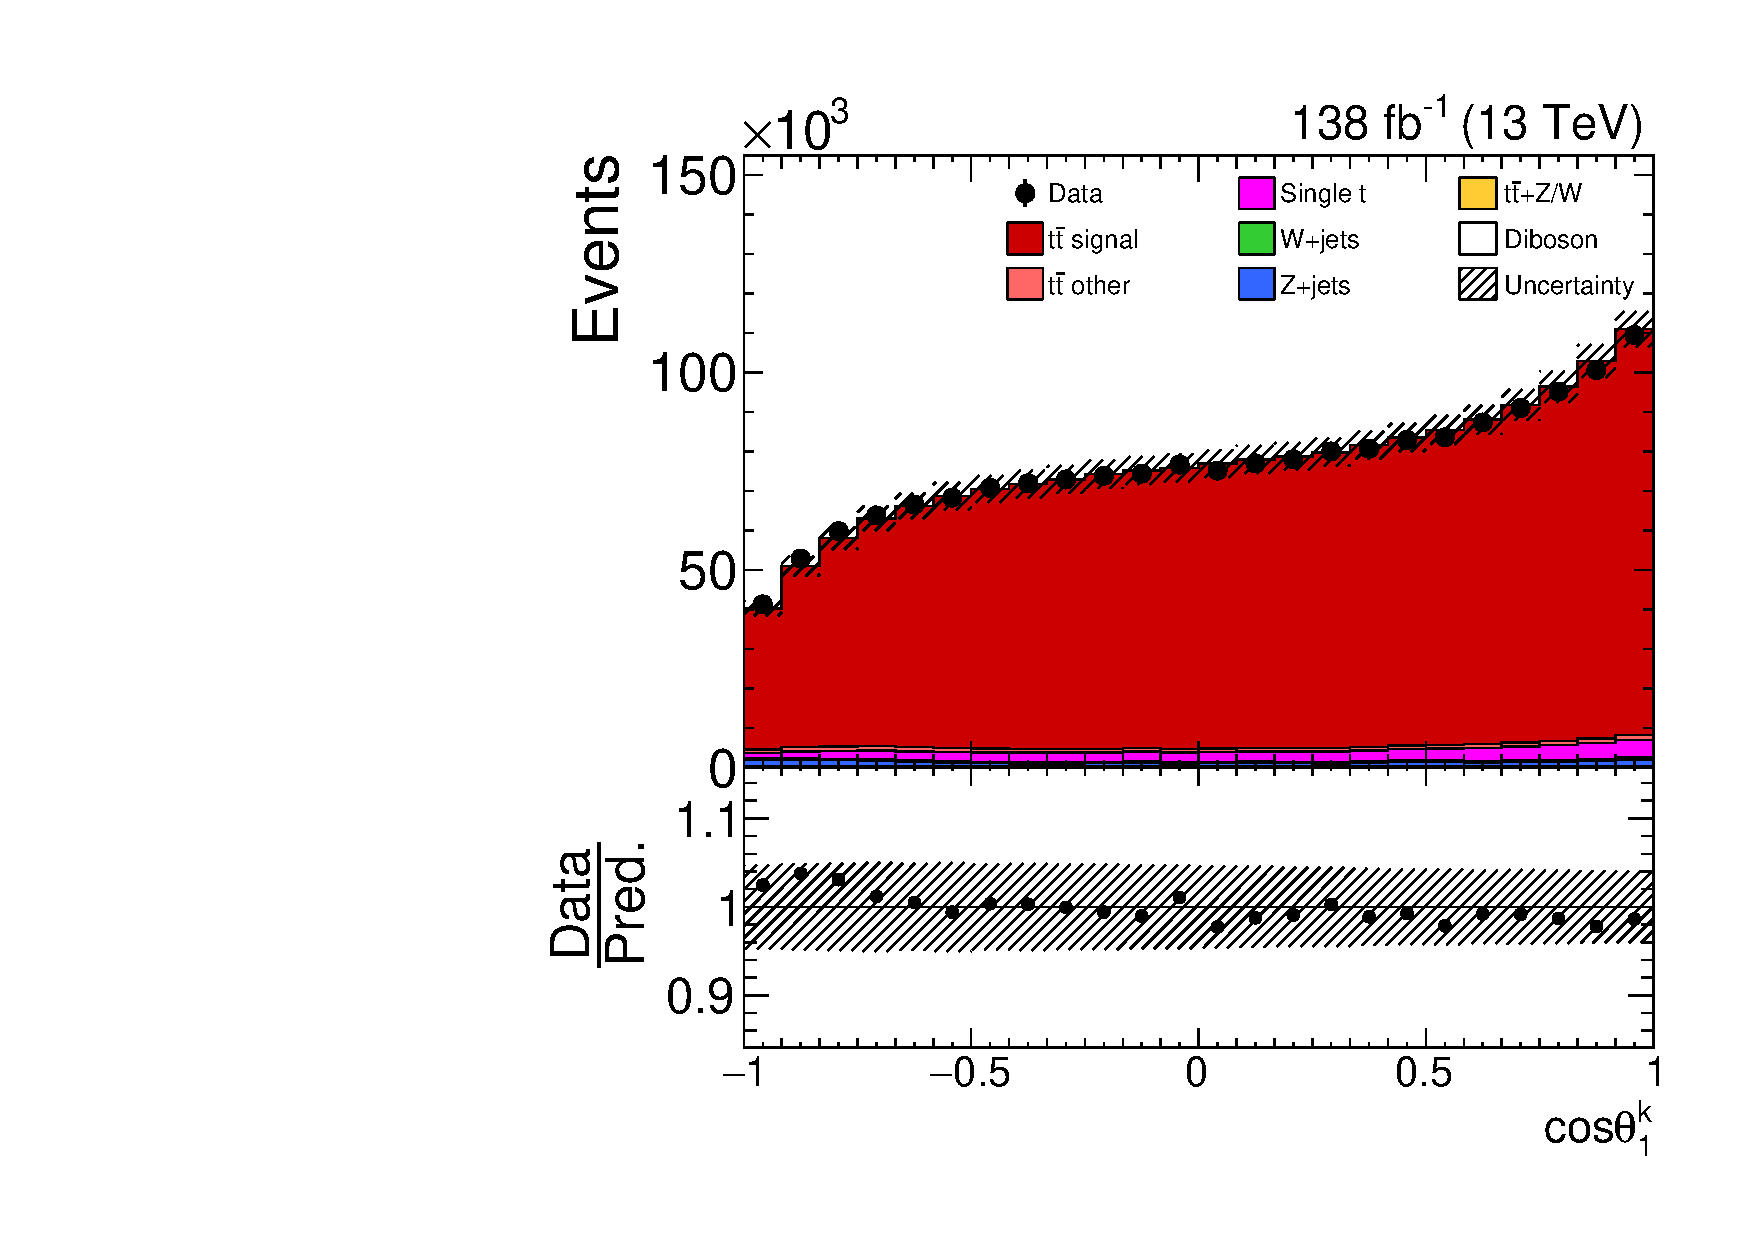
\includegraphics[width=0.40\textwidth]{fig_fullRun2UL/controlplots/combined/Hyp_AntiLeptonBk.pdf}
 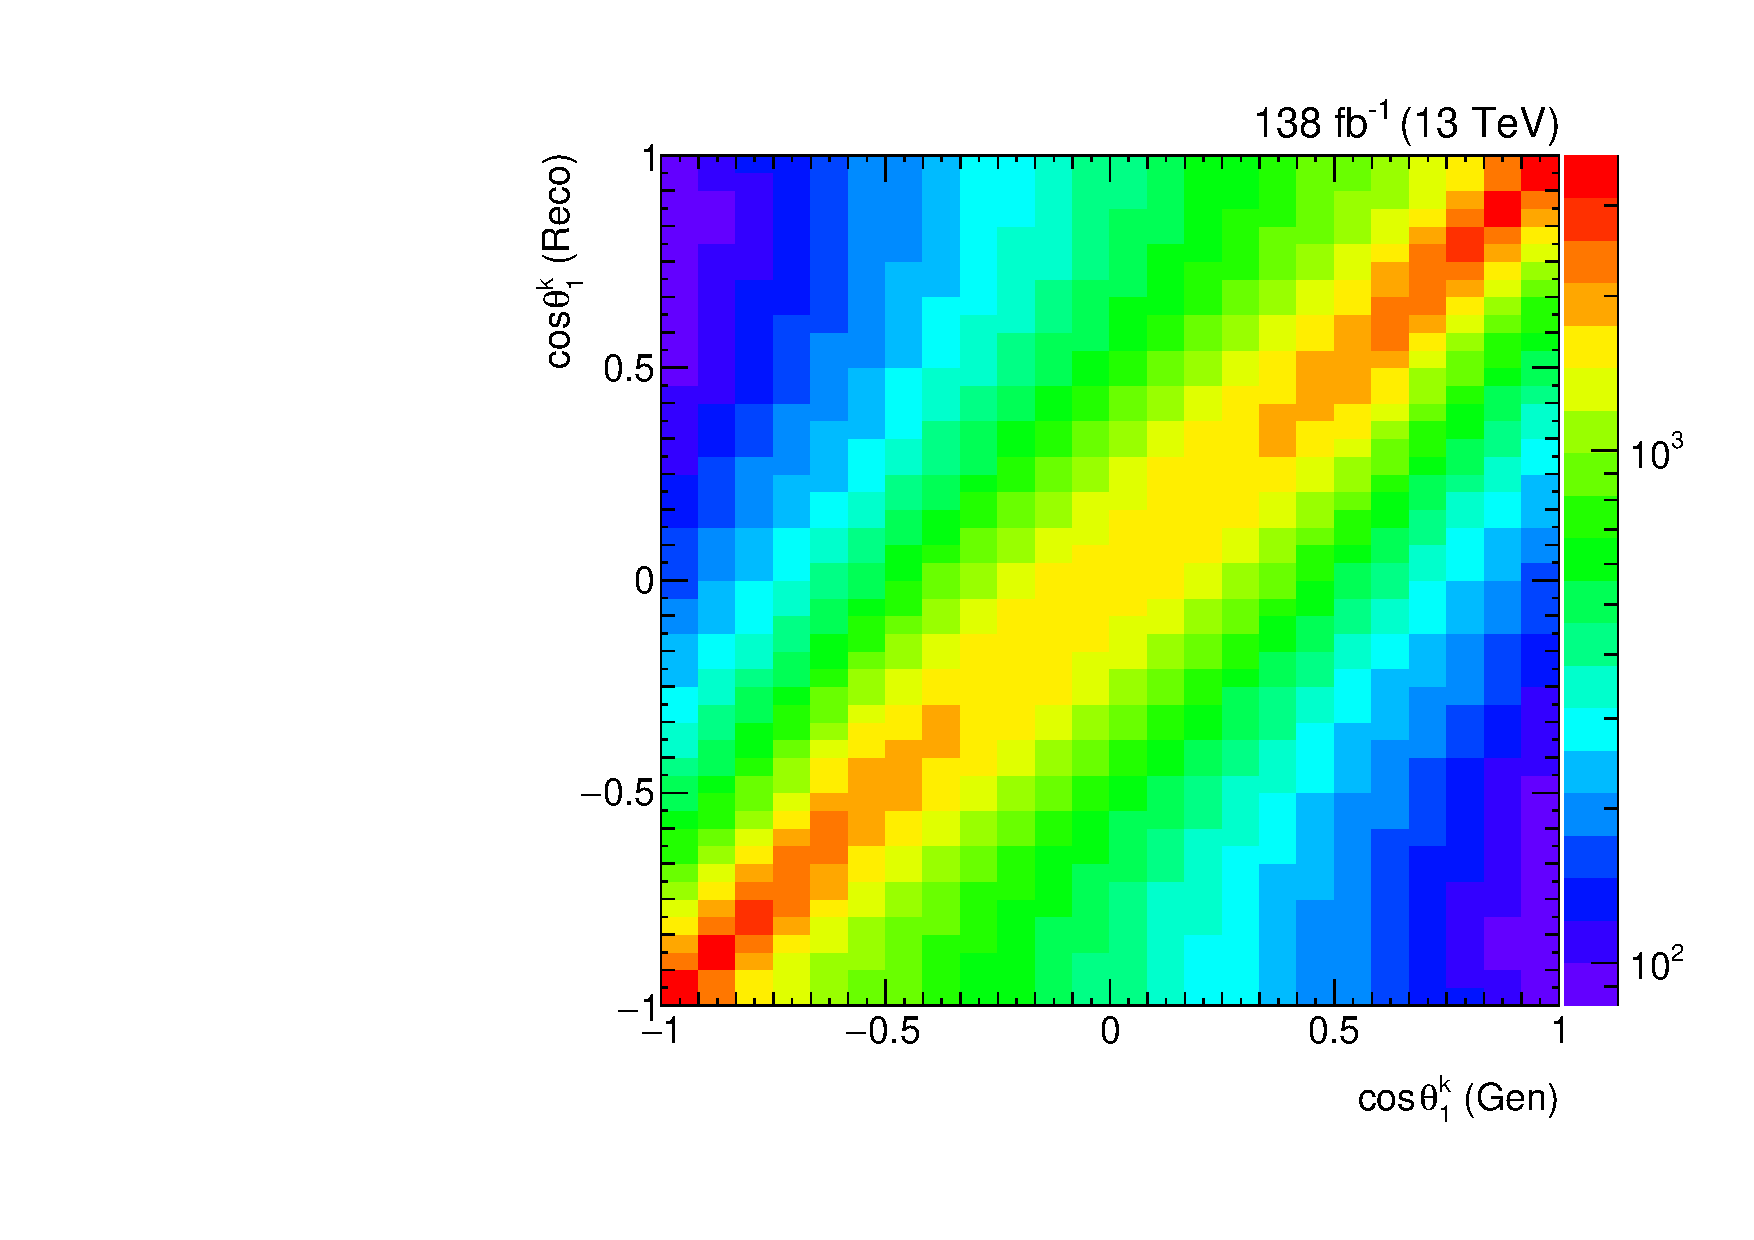
\includegraphics[width=0.40\textwidth]{fig_fullRun2UL/unfolding/combined/ResponseMatrix_b1k.pdf} \\
 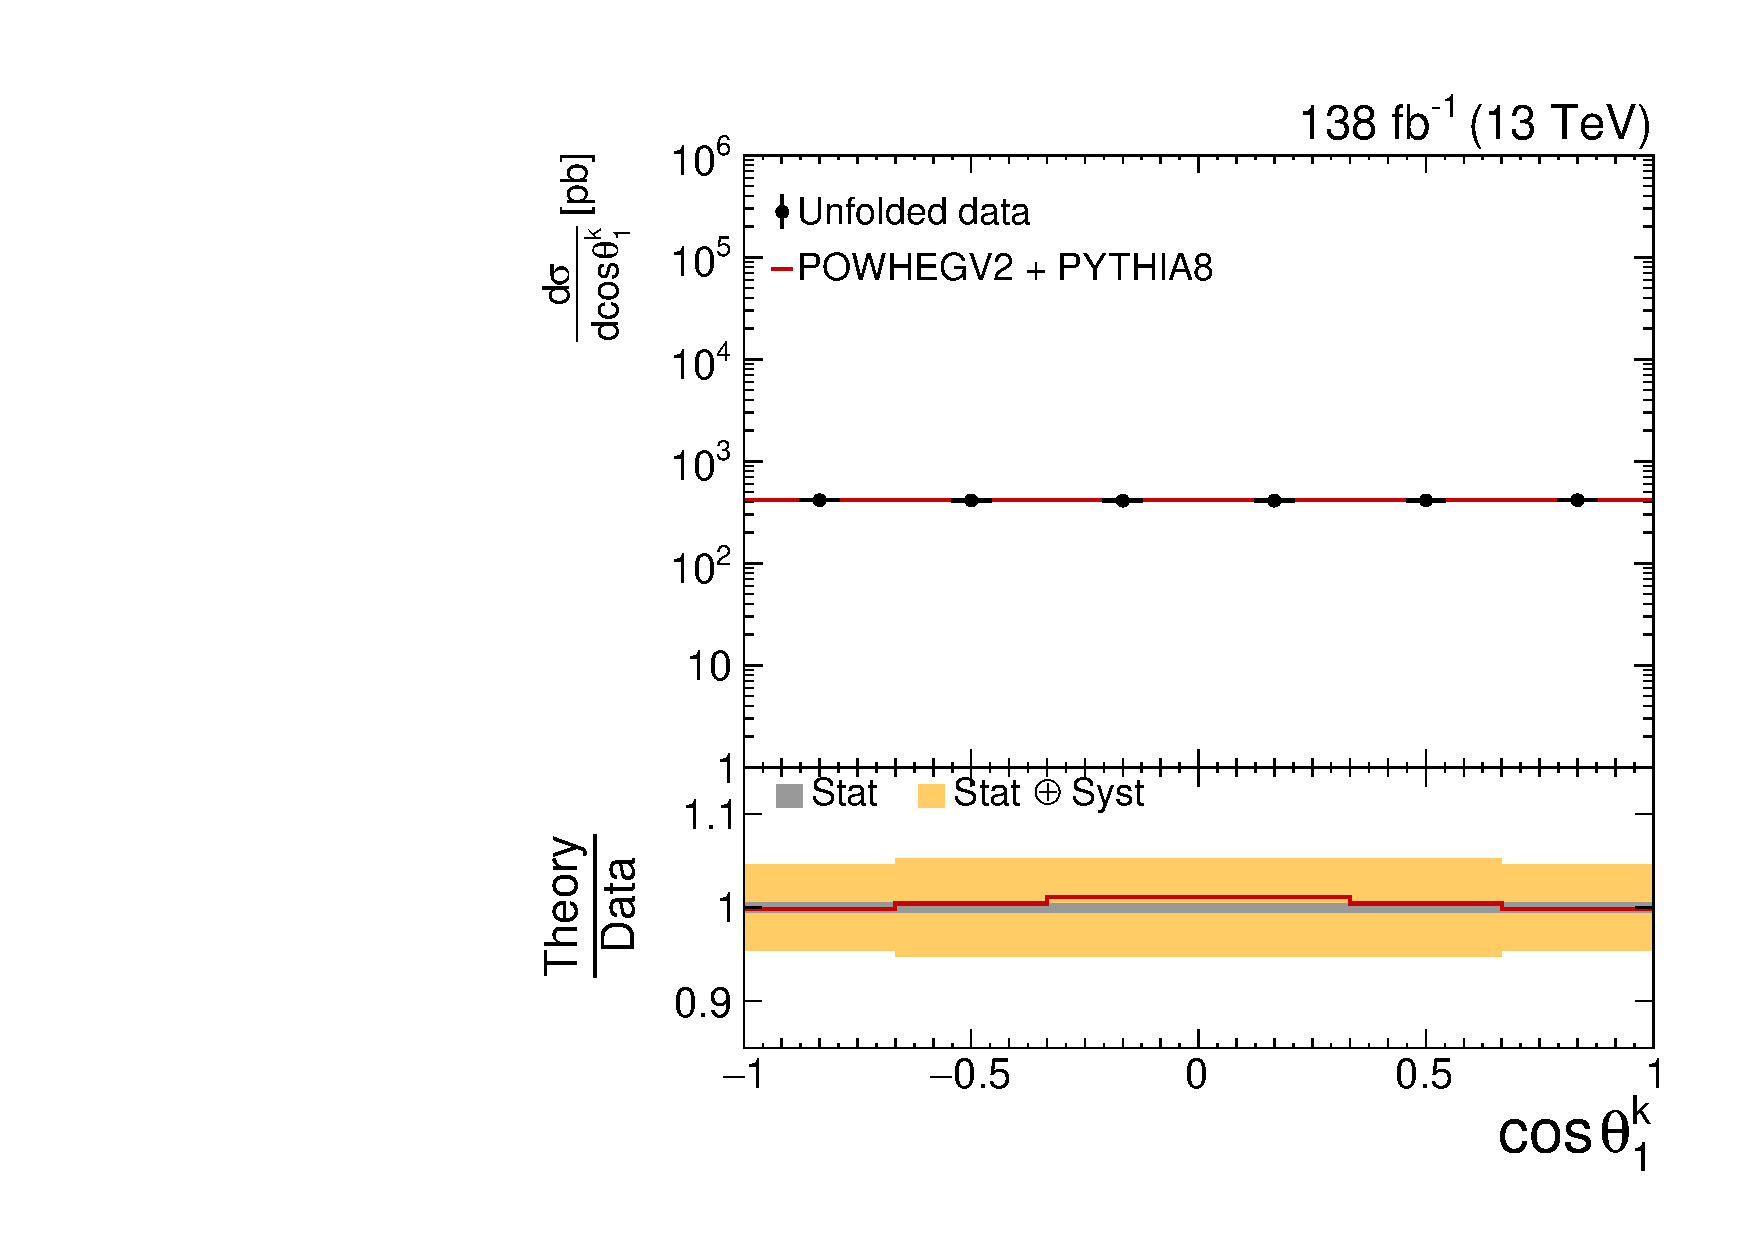
\includegraphics[width=0.40\textwidth]{fig_fullRun2UL/unfolding/combined/UnfoldedResults_b1k.pdf}
 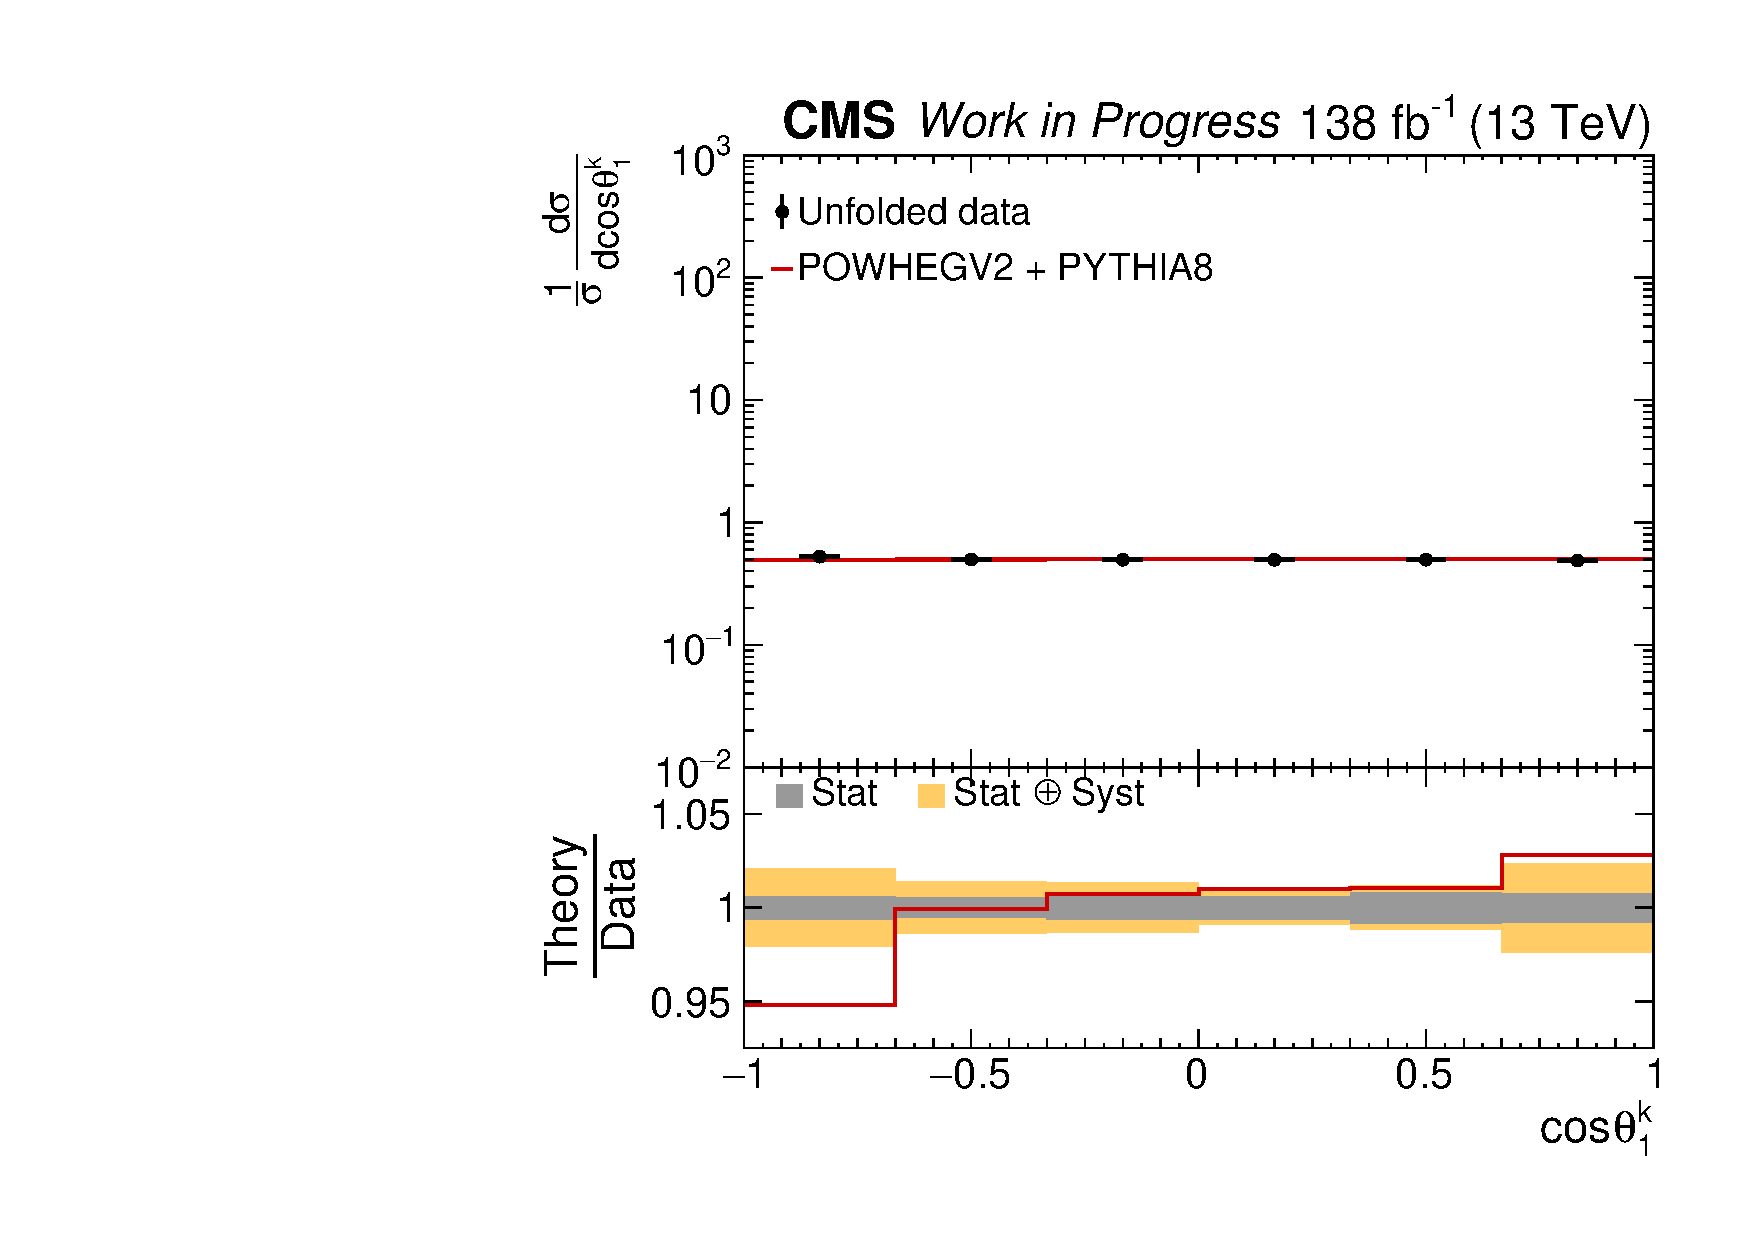
\includegraphics[width=0.40\textwidth]{fig_fullRun2UL/unfolding/combined/UnfoldedResultsNorm_b1k.pdf} \\
\label{fig:b1k}
\caption{Reconstructed detector-level distribution (Top Left), detector response-matrix (Top Right), absolute cross-section unfolded to parton-level (Bottom Left), and normalized cross-section unfolded to parton-level (Bottom Right) for polarization observable $\cos\theta_{1}^{k}$, from which spin-density coefficient $B_{1}^{k}$ (sensitive to spin-density coefficient function $b_k^{+}$) is extracted.}
\end{center}
\end{figure}
\clearpage
\begin{figure}[htb]
\begin{center}
 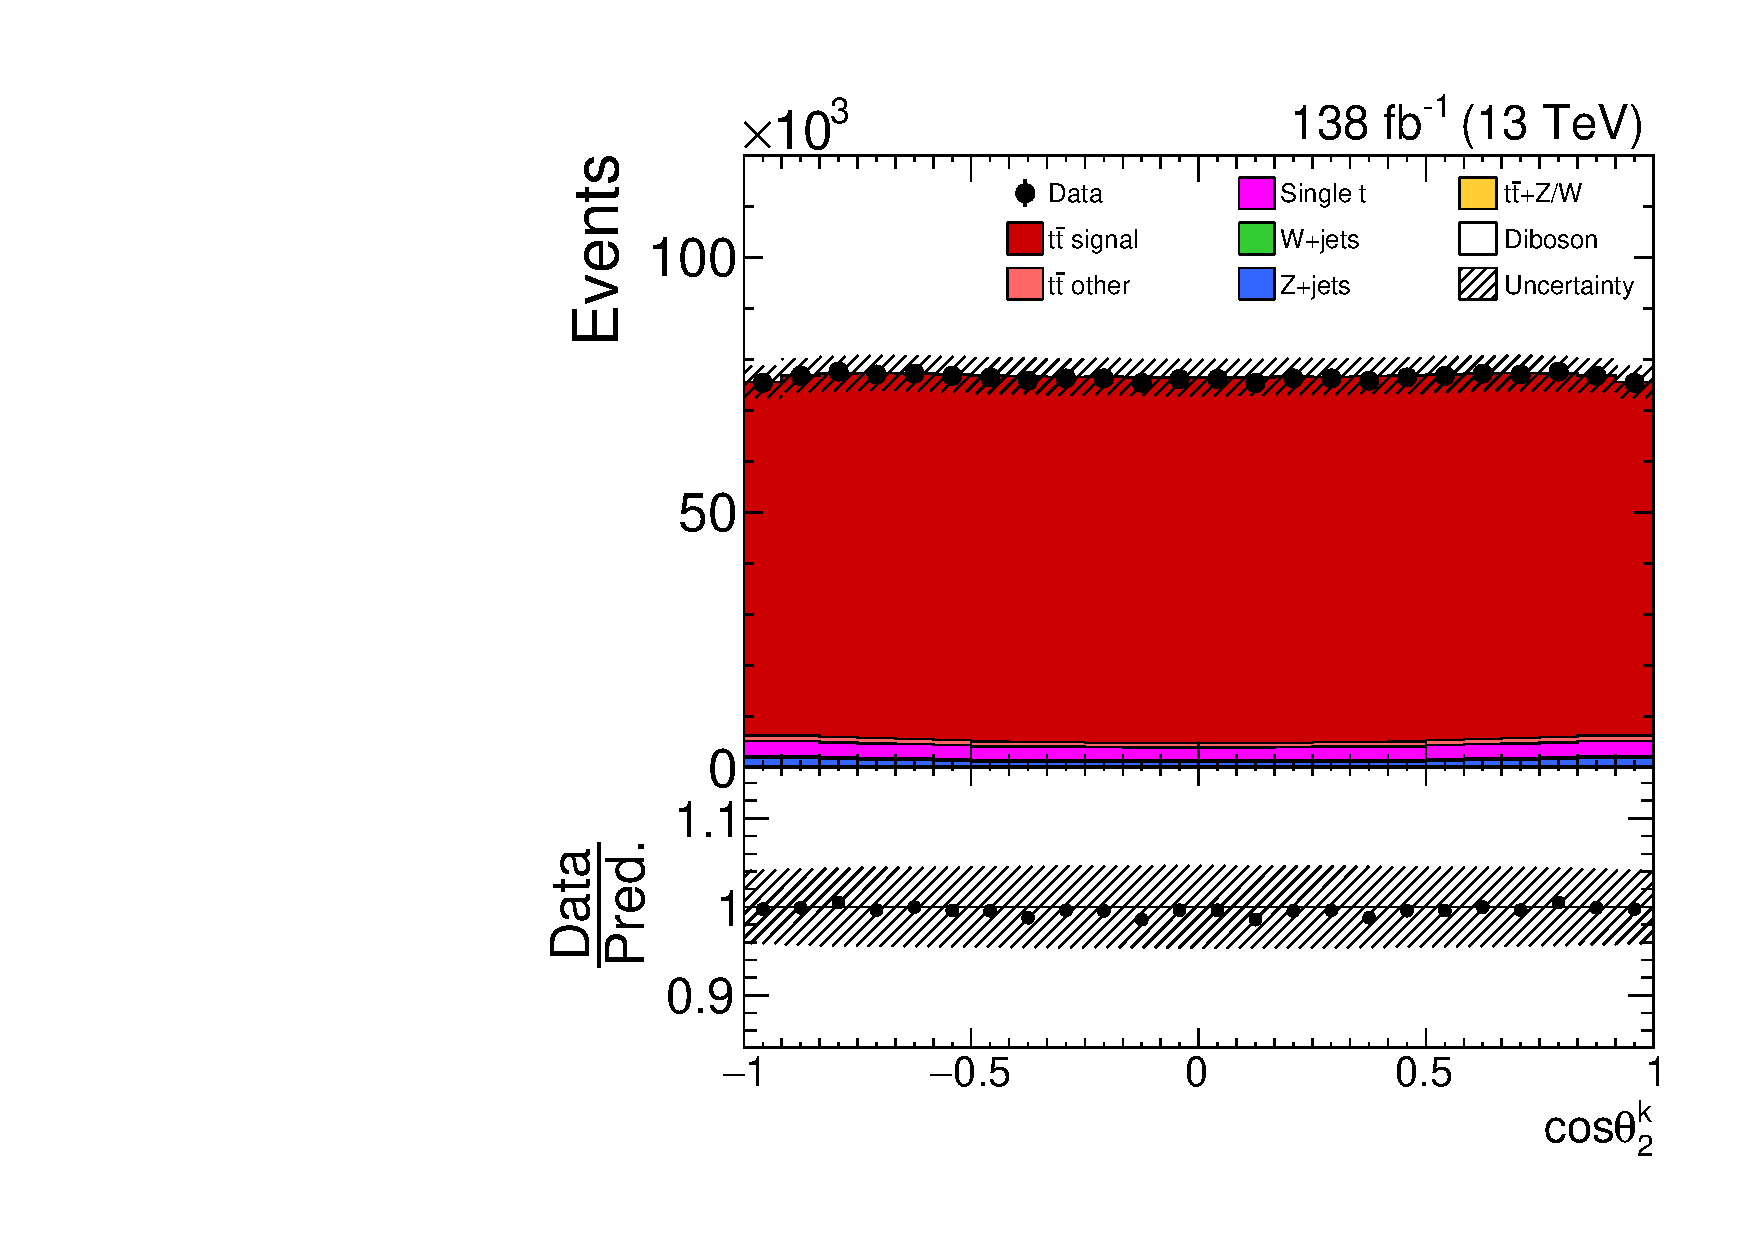
\includegraphics[width=0.40\textwidth]{fig_fullRun2UL/controlplots/combined/Hyp_LeptonBk.pdf}
 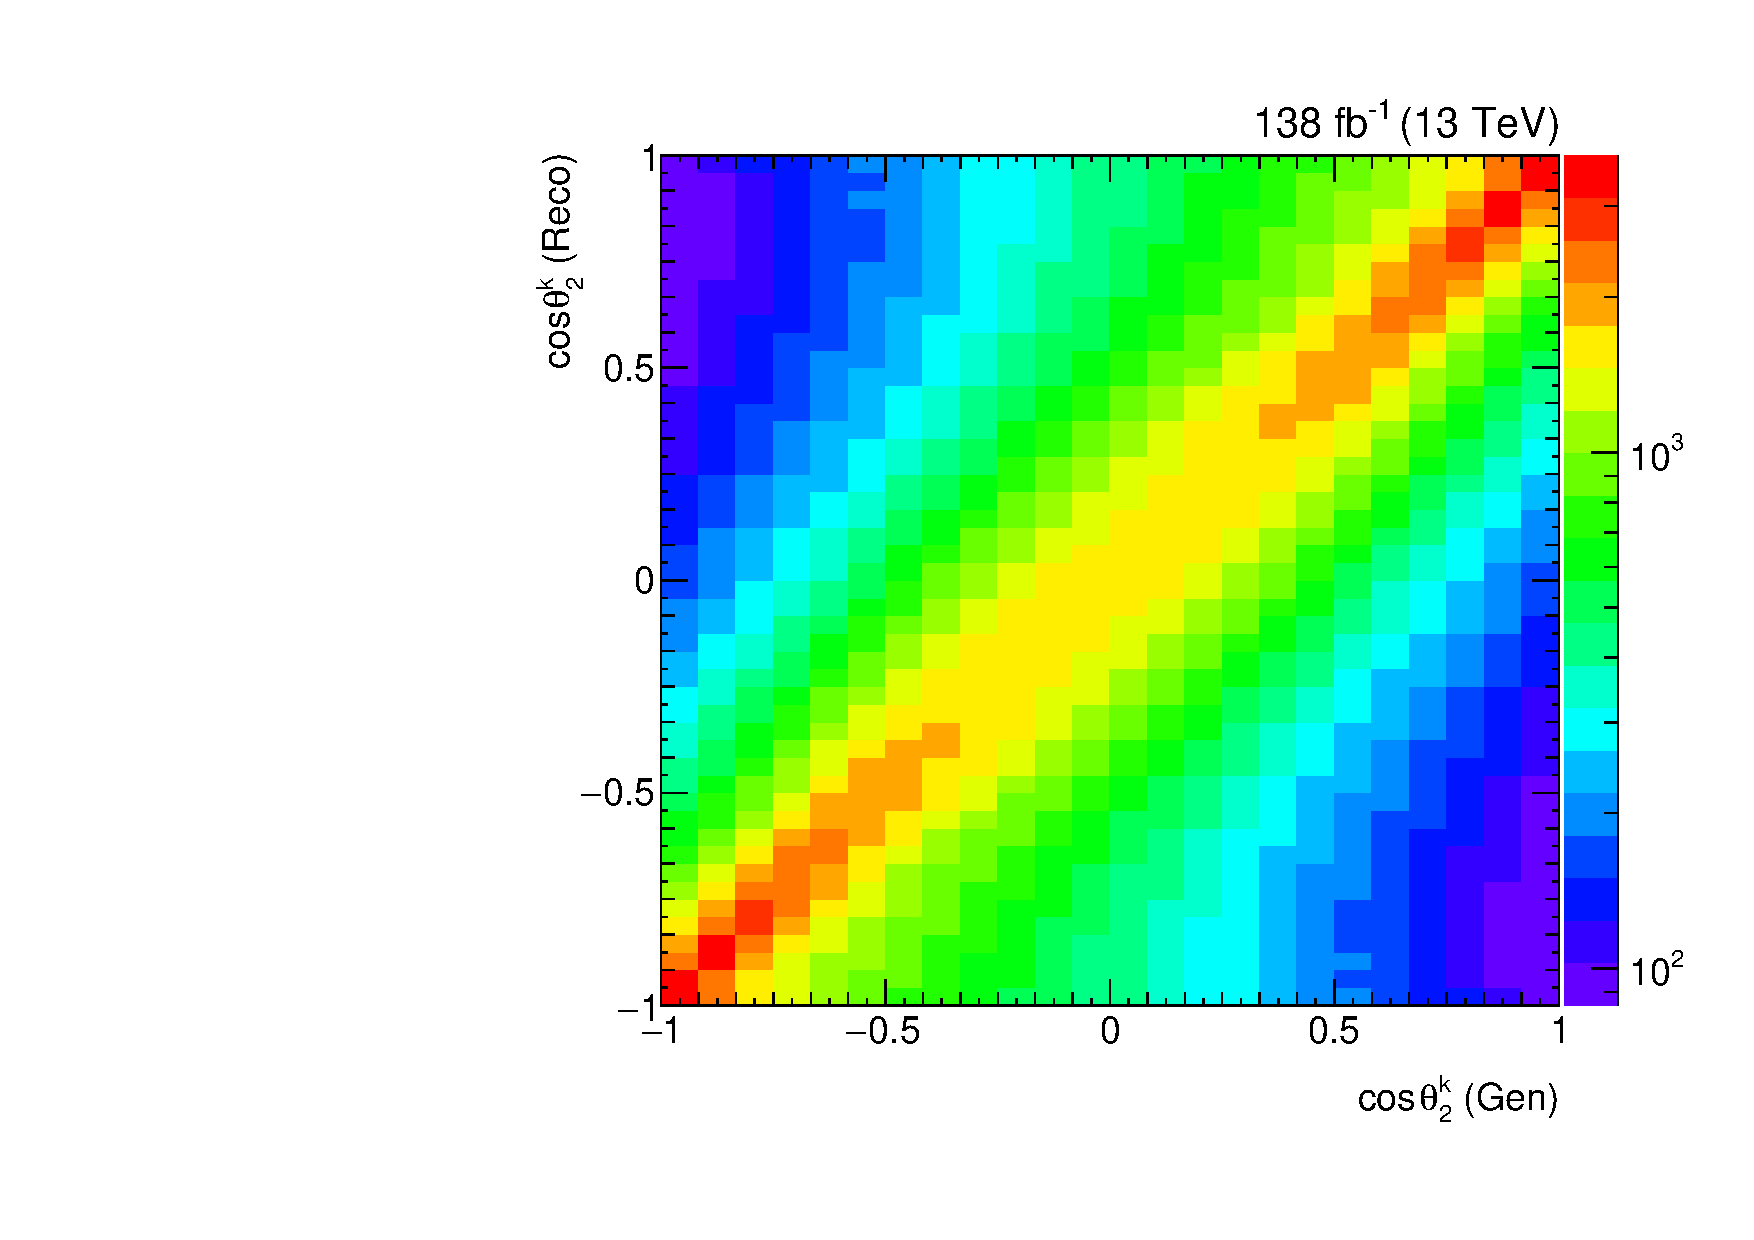
\includegraphics[width=0.40\textwidth]{fig_fullRun2UL/unfolding/combined/ResponseMatrix_b2k.pdf} \\
 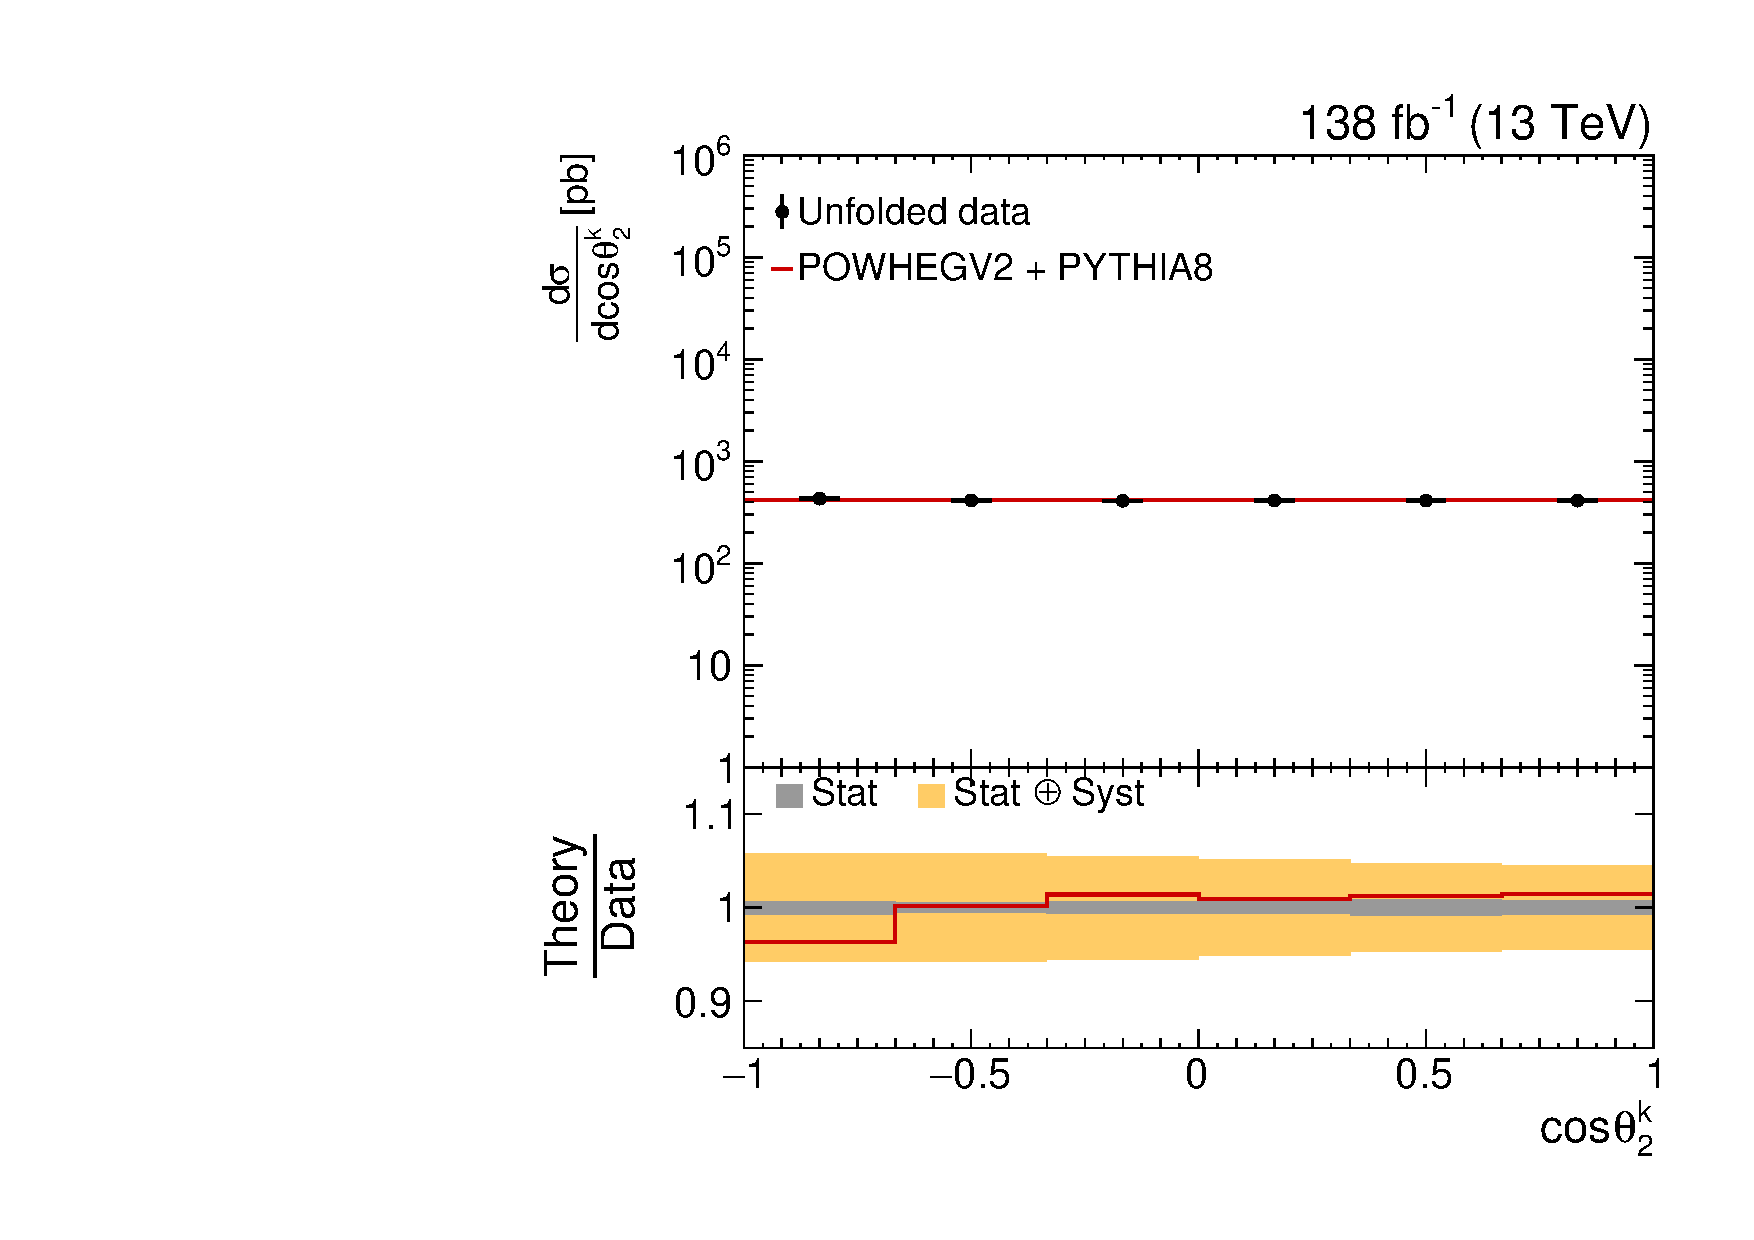
\includegraphics[width=0.40\textwidth]{fig_fullRun2UL/unfolding/combined/UnfoldedResults_b2k.pdf}
 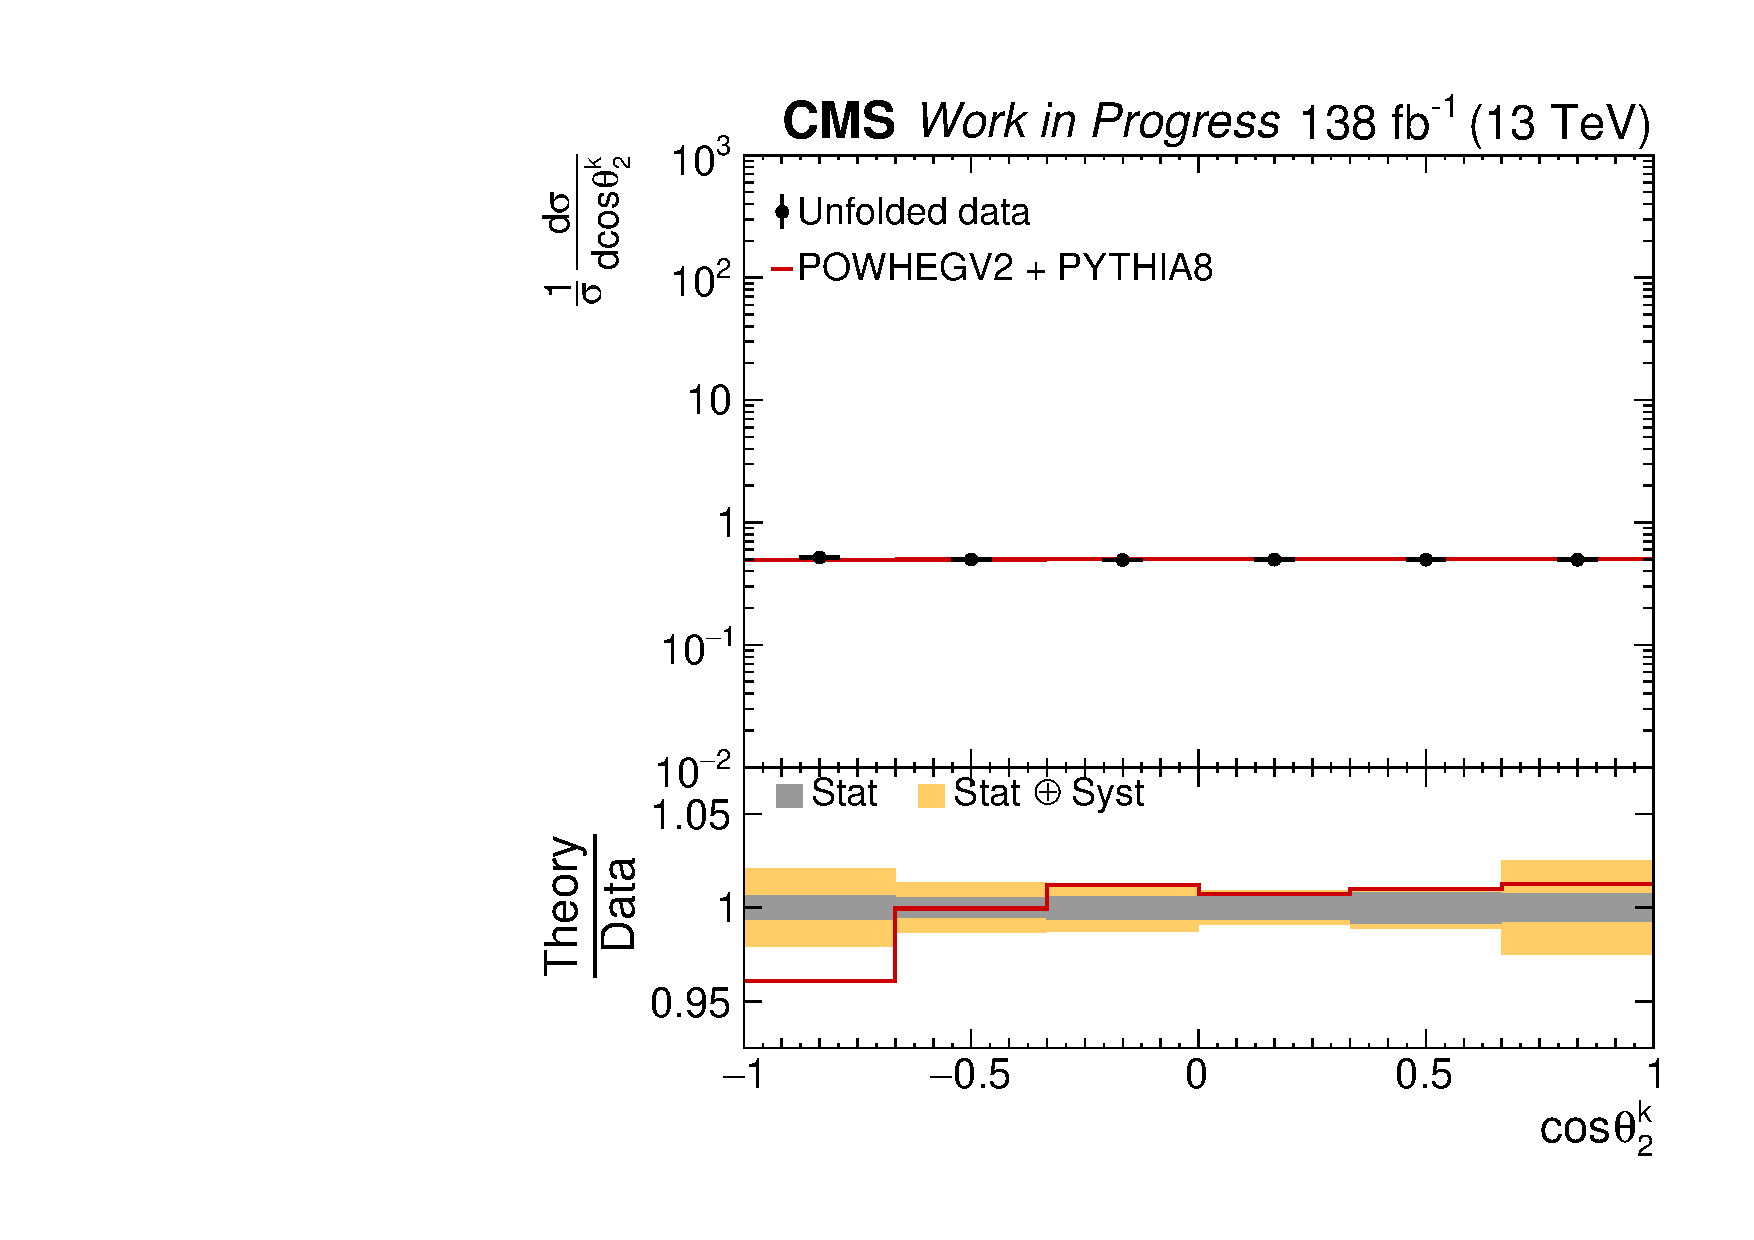
\includegraphics[width=0.40\textwidth]{fig_fullRun2UL/unfolding/combined/UnfoldedResultsNorm_b2k.pdf} \\
\label{fig:b2k}
\caption{Reconstructed detector-level distribution (Top Left), detector response-matrix (Top Right), absolute cross-section unfolded to parton-level (Bottom Left), and normalized cross-section unfolded to parton-level (Bottom Right) for polarization observable $\cos\theta_{2}^{k}$, from which spin-density coefficient $B_{2}^{k}$ (sensitive to spin-density coefficient function $b_k^{-}$) is extracted.}
\end{center}
\end{figure}
\clearpage
\begin{figure}[htb]
\begin{center}
 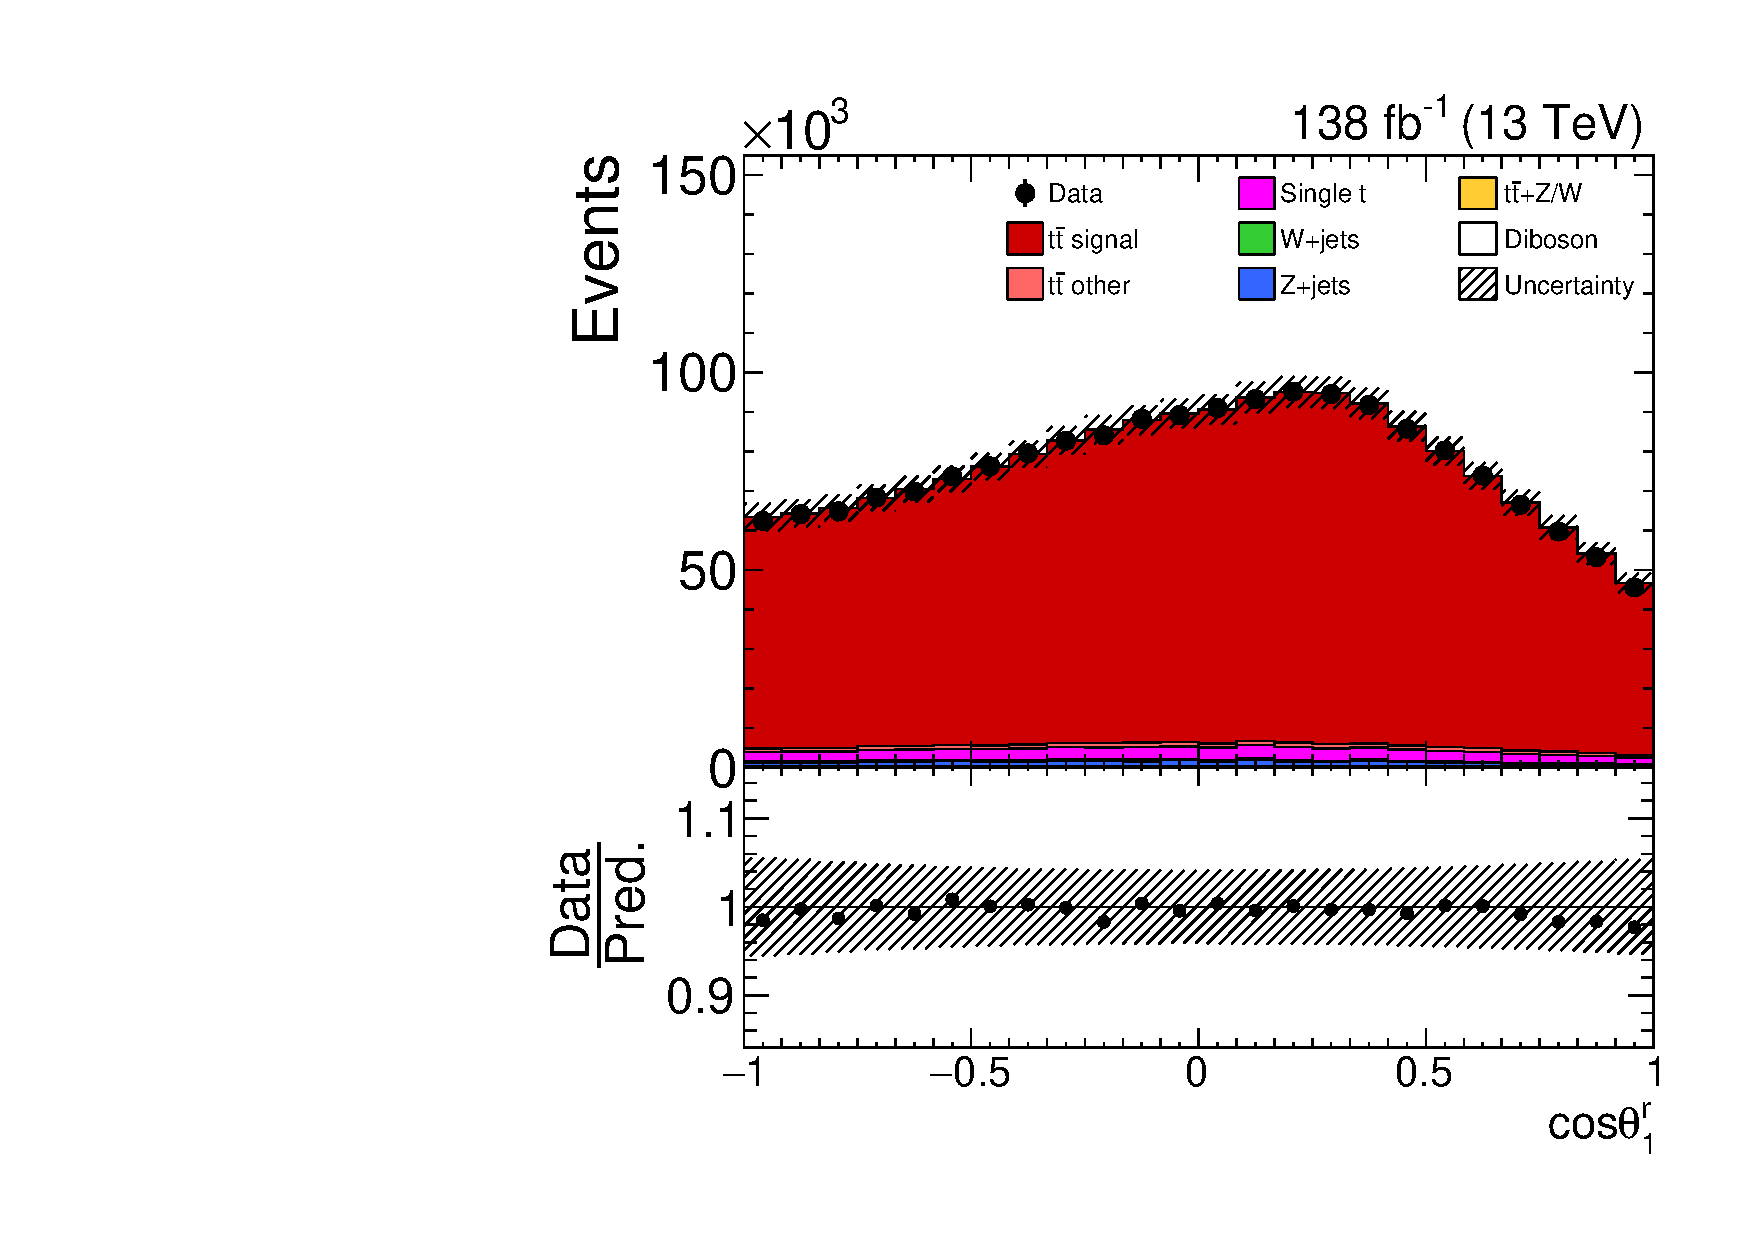
\includegraphics[width=0.40\textwidth]{fig_fullRun2UL/controlplots/combined/Hyp_AntiLeptonBr.pdf}
 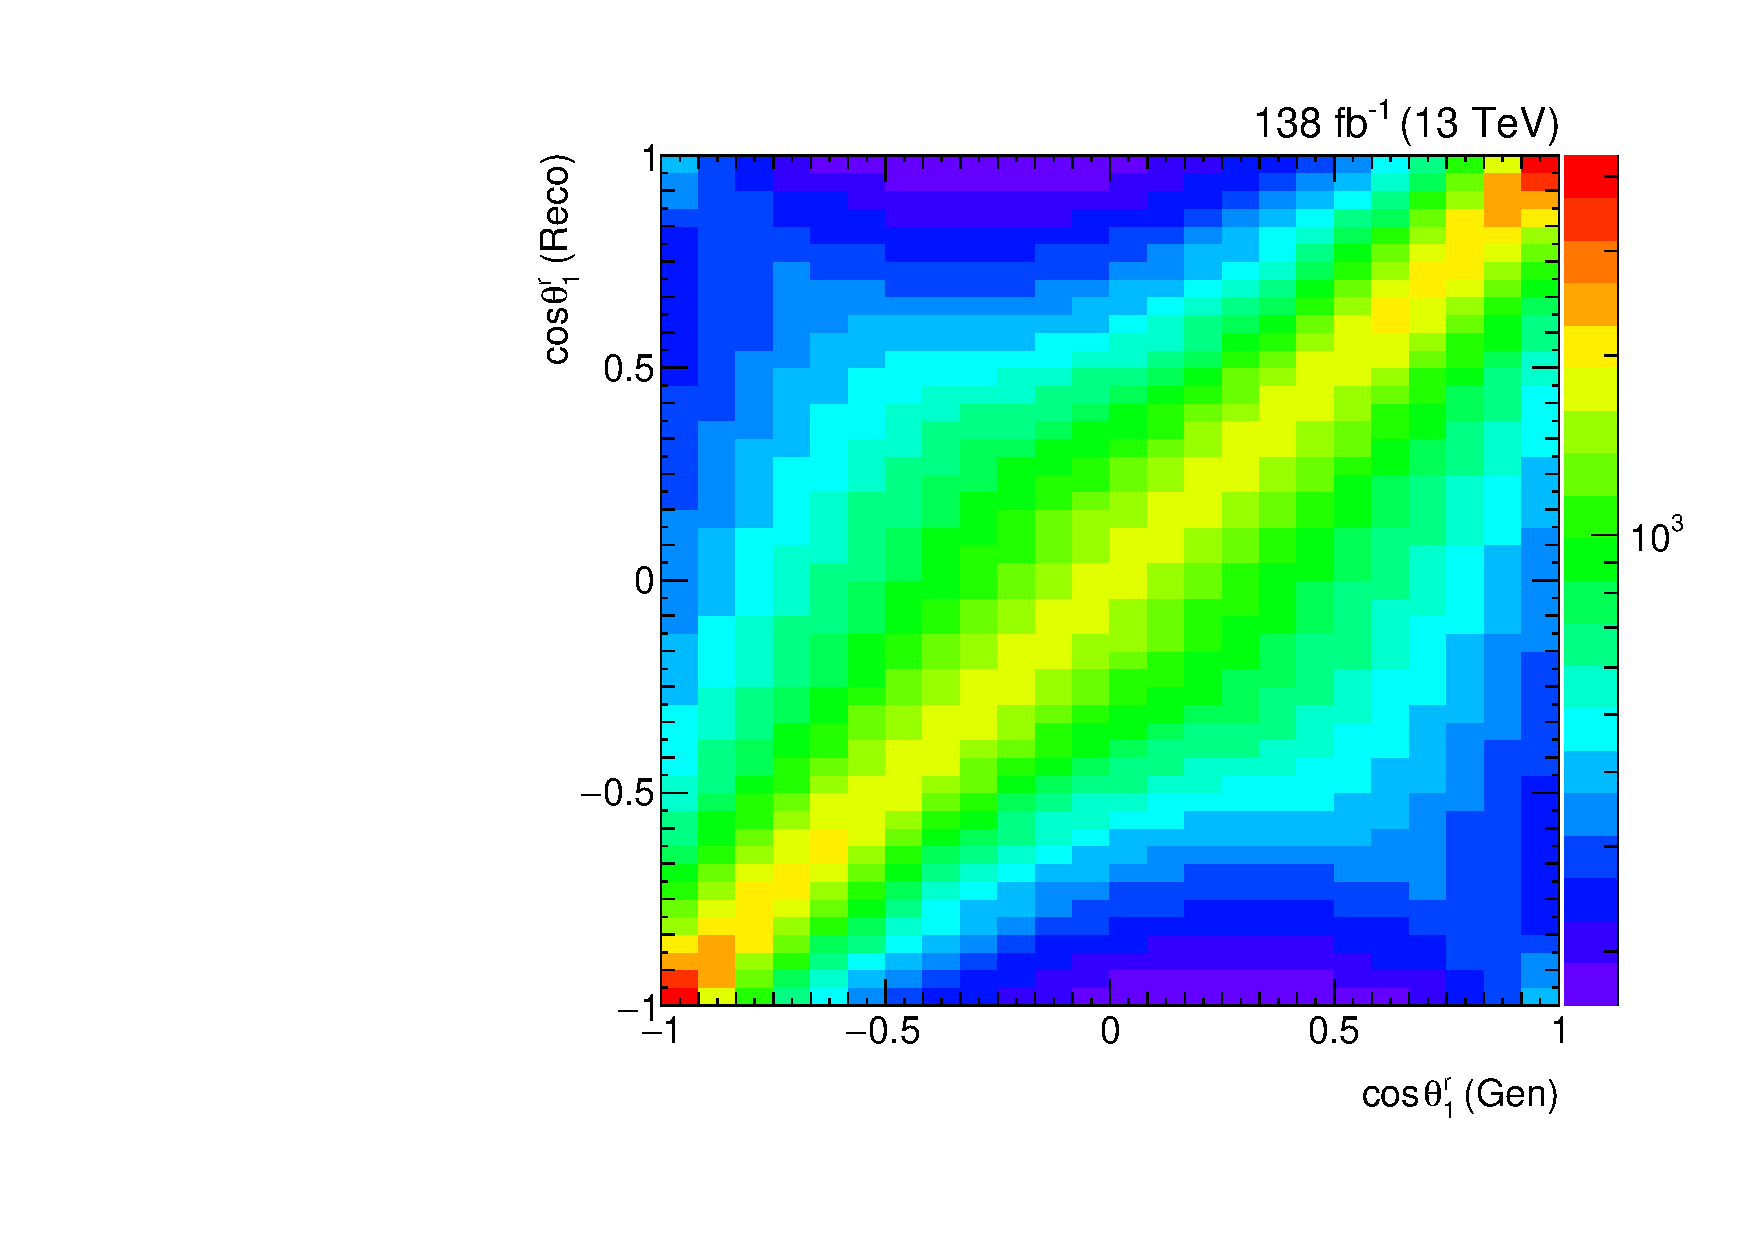
\includegraphics[width=0.40\textwidth]{fig_fullRun2UL/unfolding/combined/ResponseMatrix_b1r.pdf} \\
 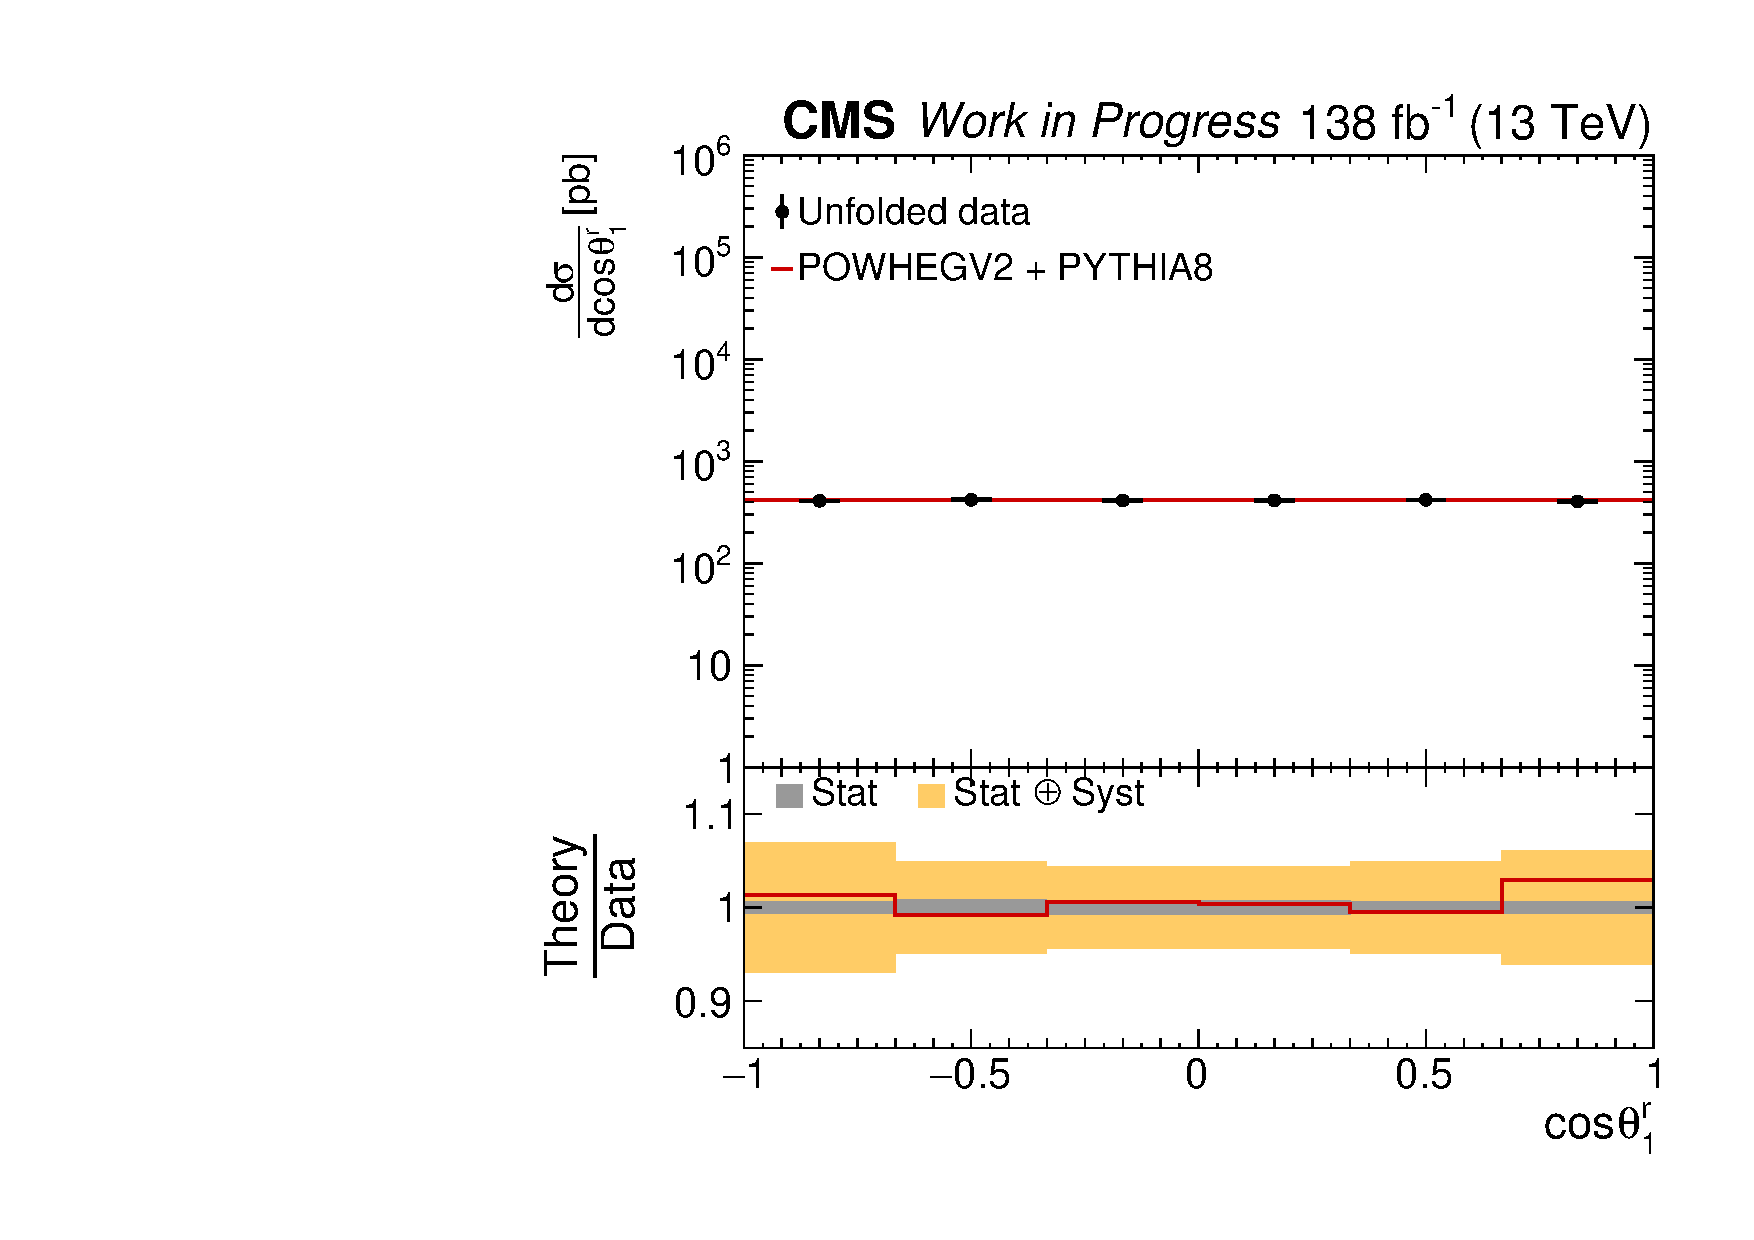
\includegraphics[width=0.40\textwidth]{fig_fullRun2UL/unfolding/combined/UnfoldedResults_b1r.pdf}
 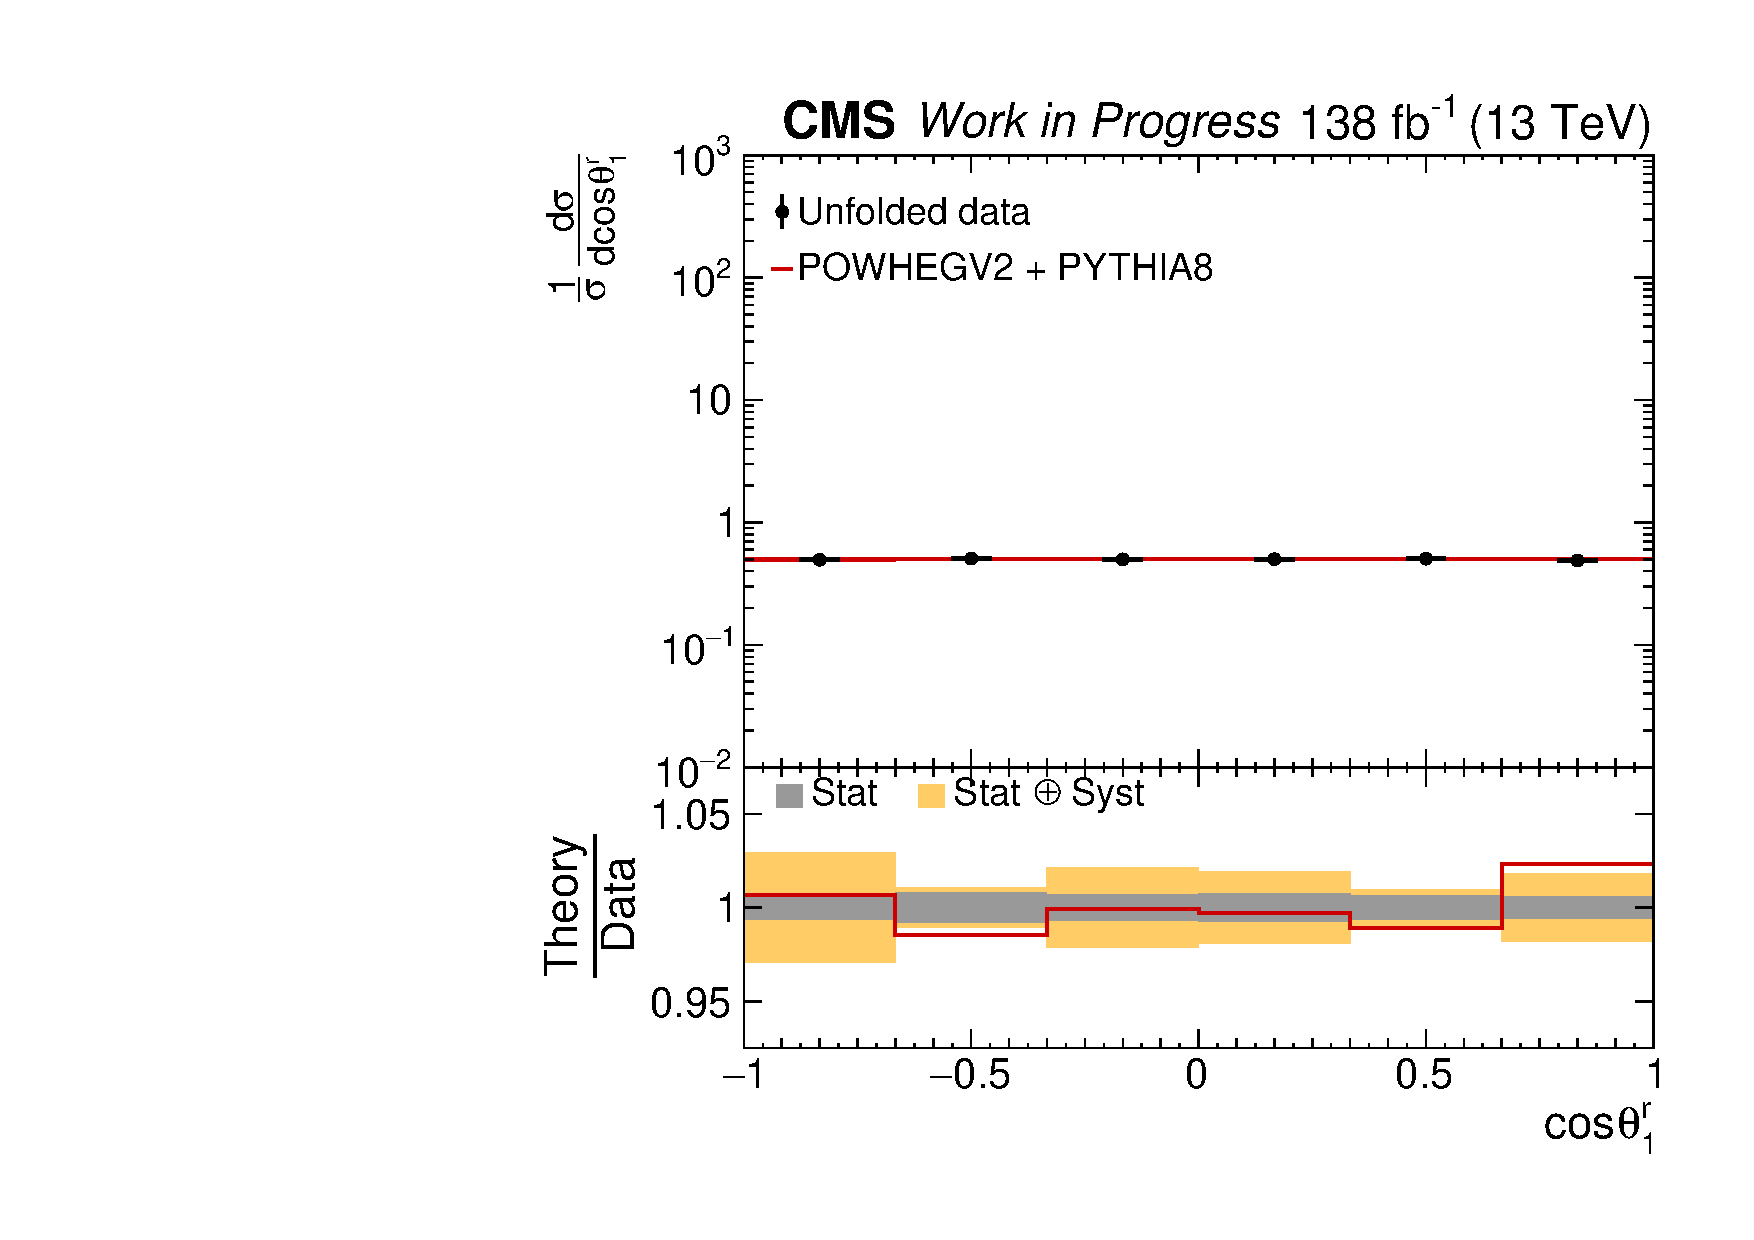
\includegraphics[width=0.40\textwidth]{fig_fullRun2UL/unfolding/combined/UnfoldedResultsNorm_b1r.pdf} \\
\label{fig:b1r}
\caption{Reconstructed detector-level distribution (Top Left), detector response-matrix (Top Right), absolute cross-section unfolded to parton-level (Bottom Left), and normalized cross-section unfolded to parton-level (Bottom Right) for polarization observable $\cos\theta_{1}^{r}$, from which spin-density coefficient $B_{1}^{r}$ (sensitive to spin-density coefficient function $b_r^{+}$) is extracted.}
\end{center}
\end{figure}
\clearpage
\begin{figure}[htb]
\begin{center}
 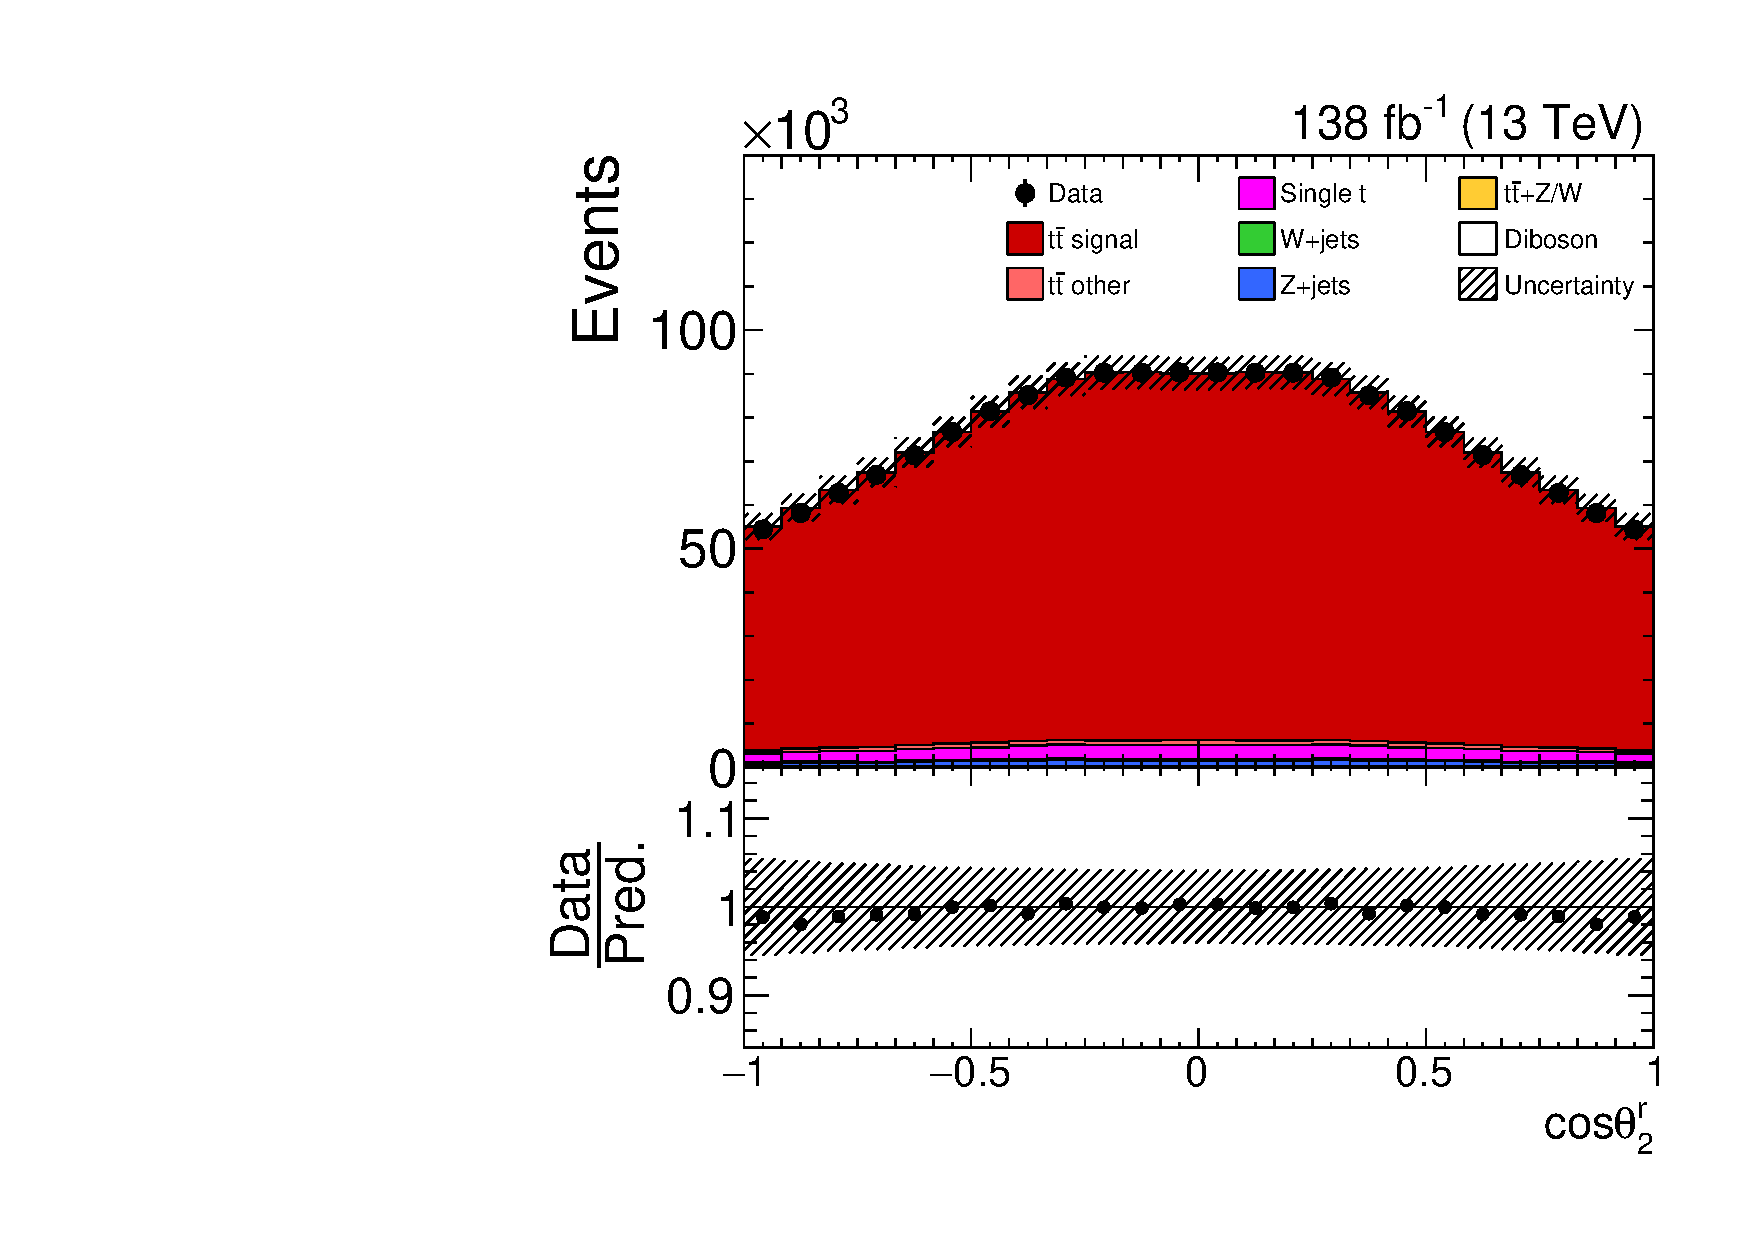
\includegraphics[width=0.40\textwidth]{fig_fullRun2UL/controlplots/combined/Hyp_LeptonBr.pdf}
 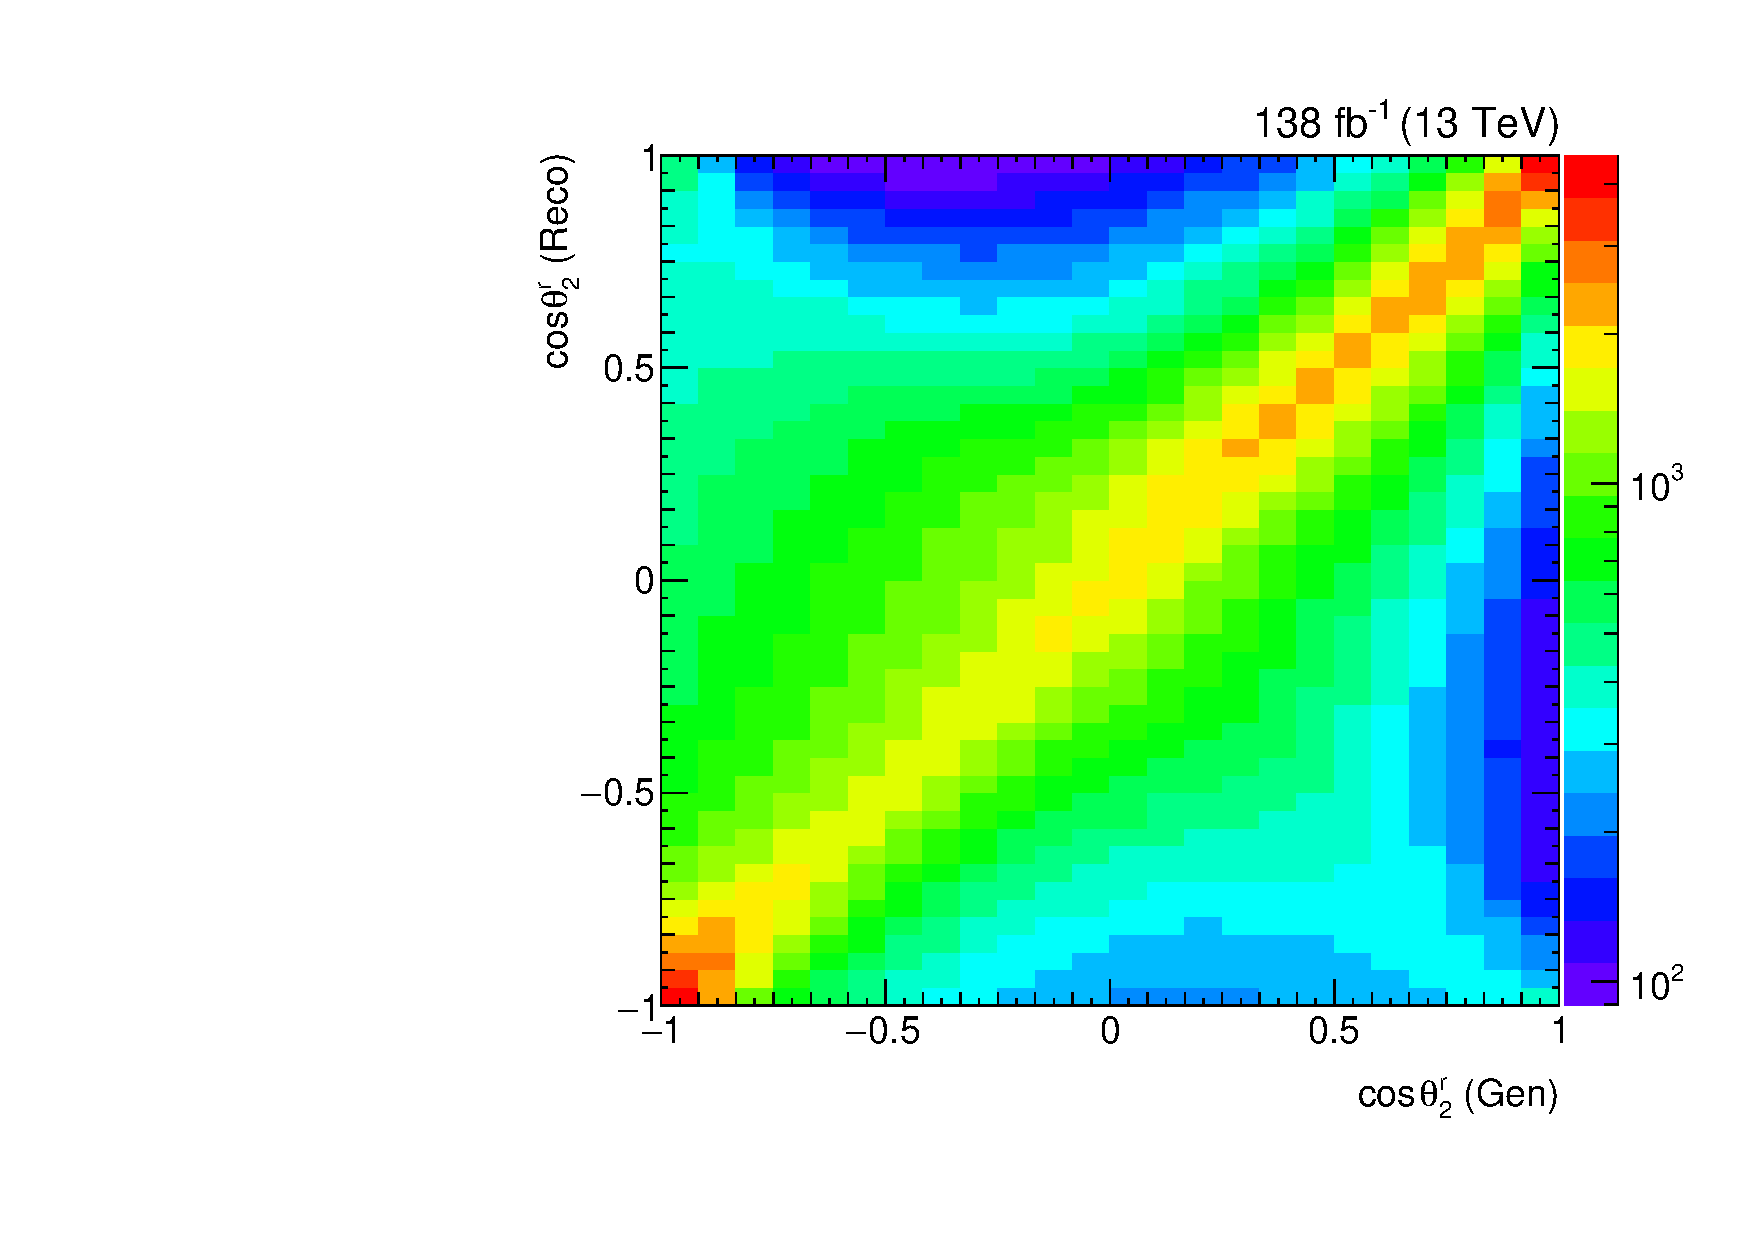
\includegraphics[width=0.40\textwidth]{fig_fullRun2UL/unfolding/combined/ResponseMatrix_b2r.pdf} \\
 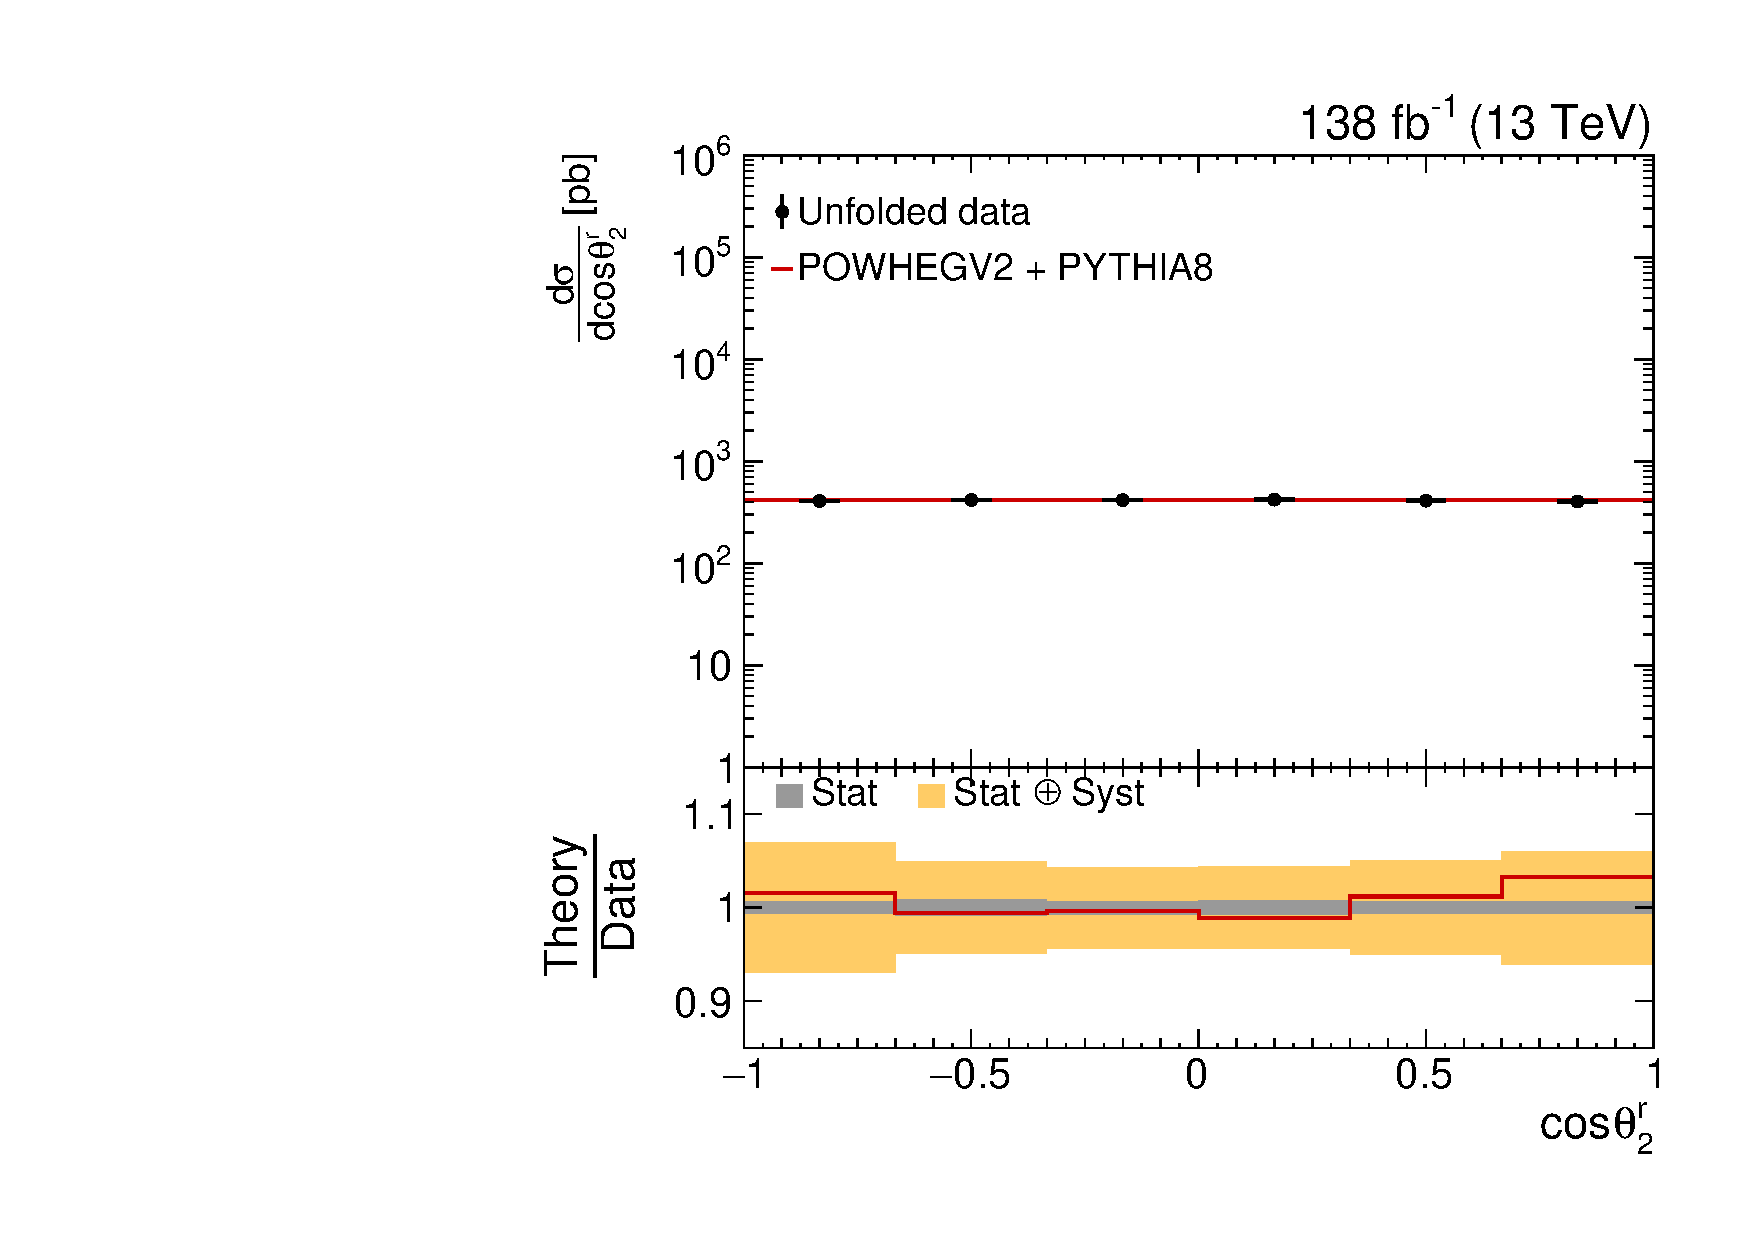
\includegraphics[width=0.40\textwidth]{fig_fullRun2UL/unfolding/combined/UnfoldedResults_b2r.pdf}
 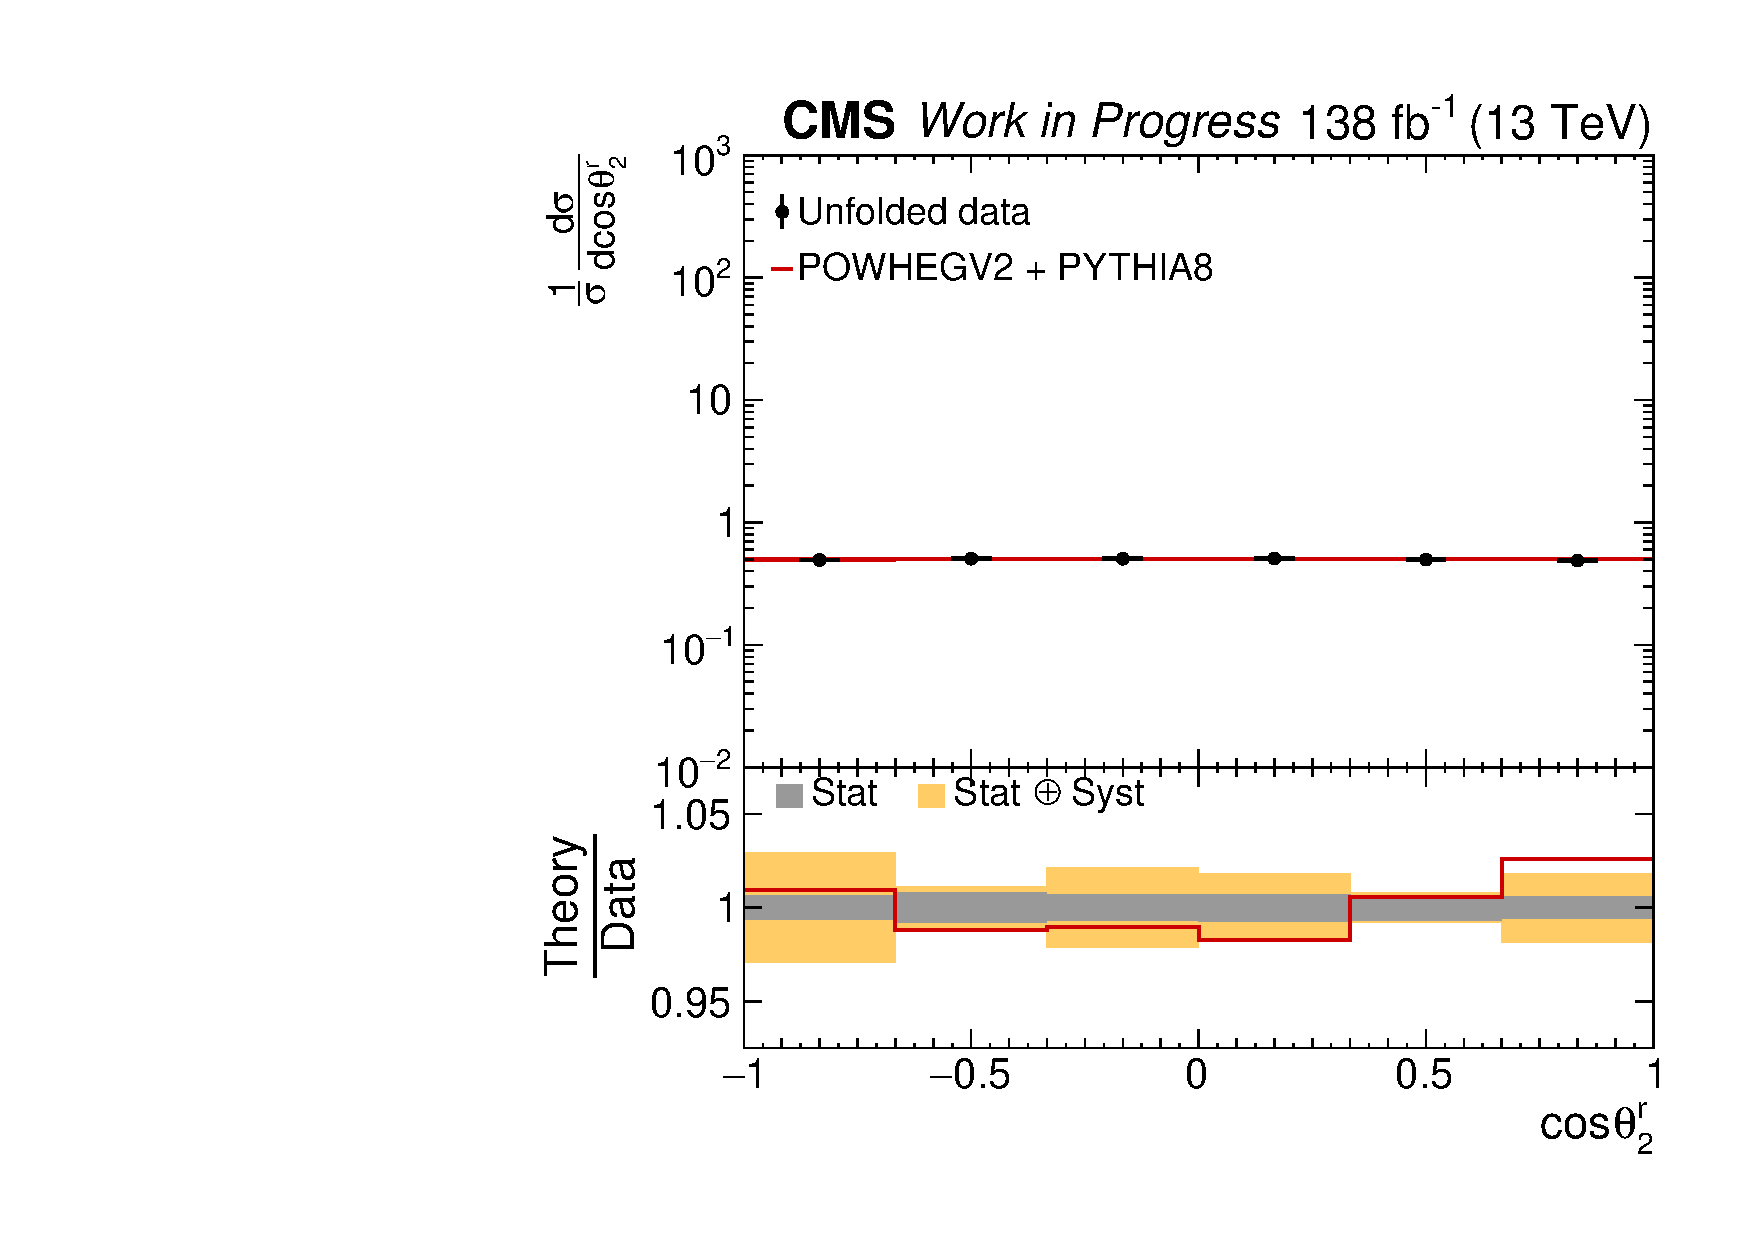
\includegraphics[width=0.40\textwidth]{fig_fullRun2UL/unfolding/combined/UnfoldedResultsNorm_b2r.pdf} \\
\label{fig:b2r}
\caption{Reconstructed detector-level distribution (Top Left), detector response-matrix (Top Right), absolute cross-section unfolded to parton-level (Bottom Left), and normalized cross-section unfolded to parton-level (Bottom Right) for polarization observable $\cos\theta_{2}^{r}$, from which spin-density coefficient $B_{2}^{r}$ (sensitive to spin-density coefficient function $b_r^{-}$) is extracted.}
\end{center}
\end{figure}
\clearpage
\begin{figure}[htb]
\begin{center}
 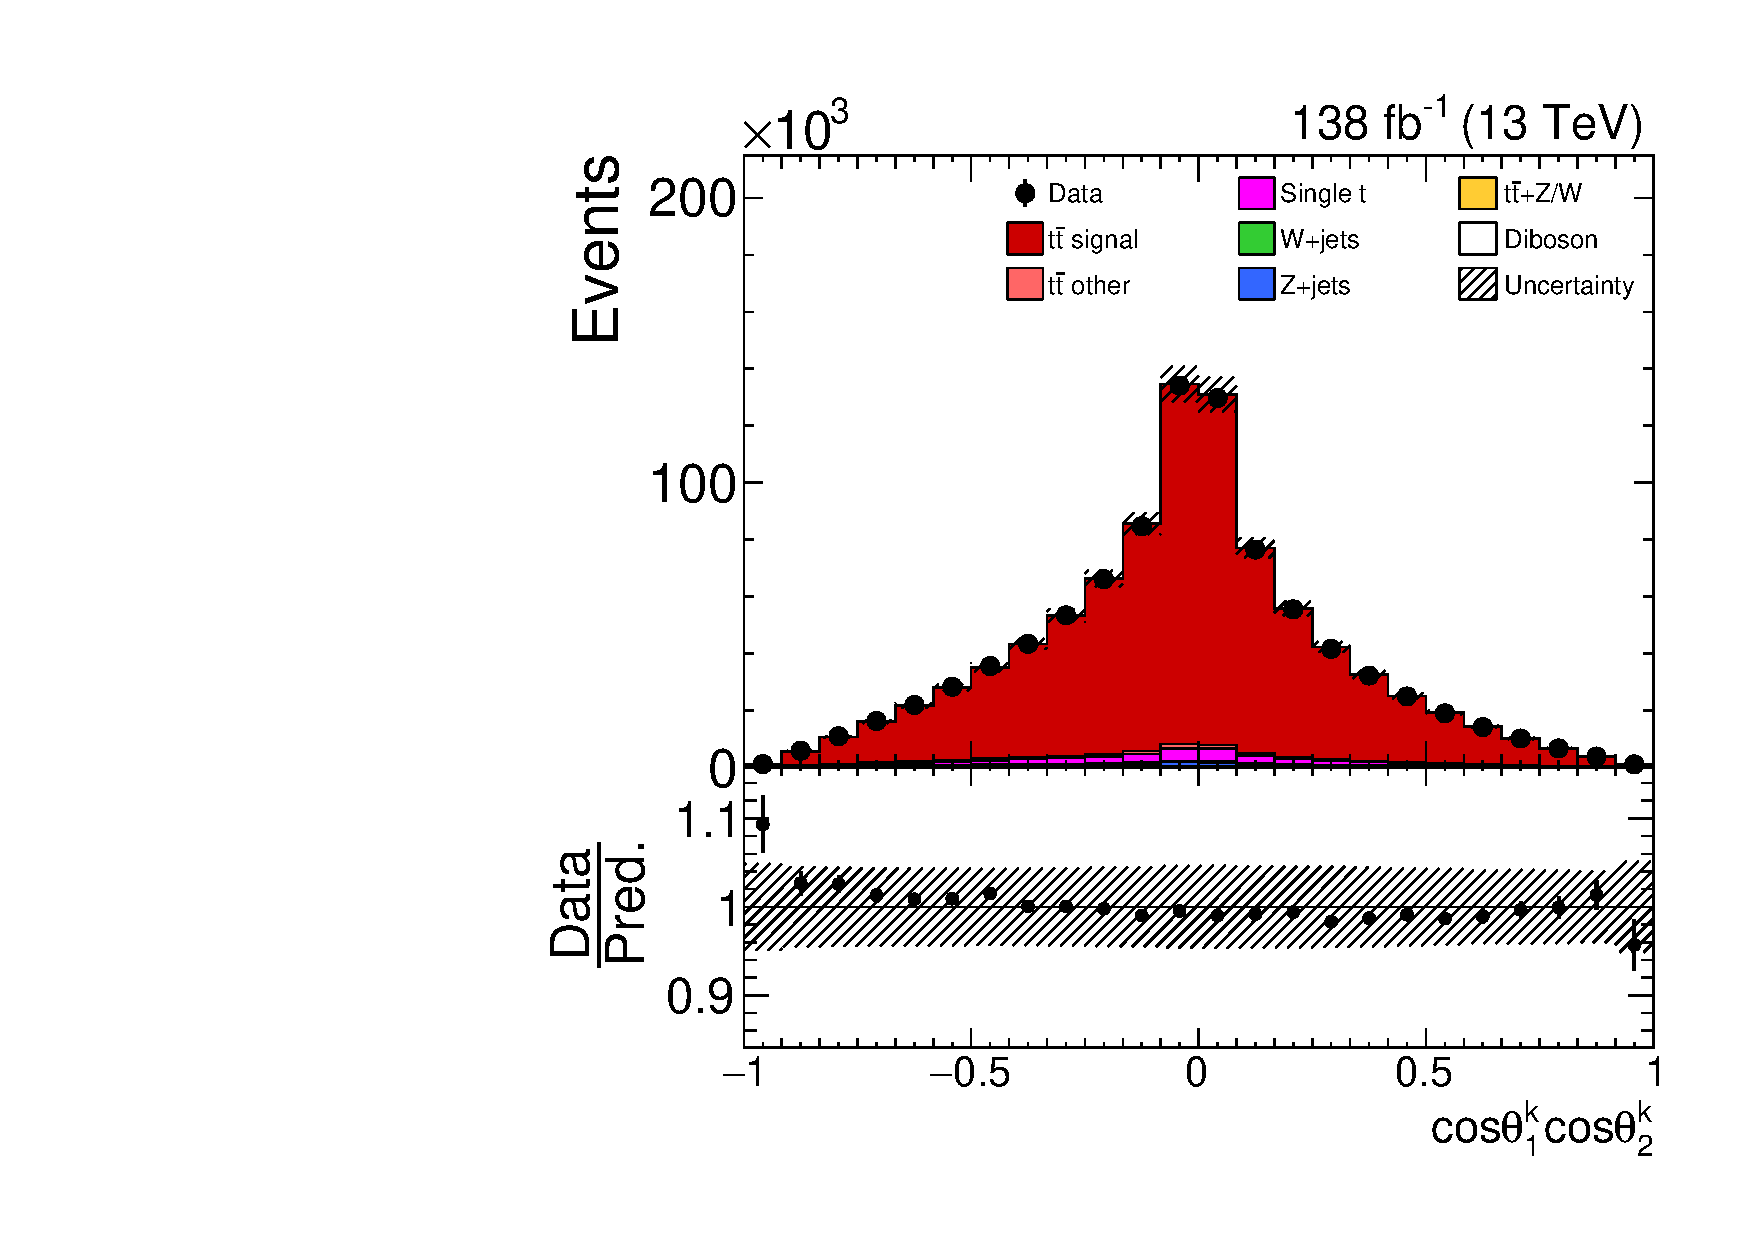
\includegraphics[width=0.40\textwidth]{fig_fullRun2UL/controlplots/combined/Hyp_LLBarCkk.pdf}
 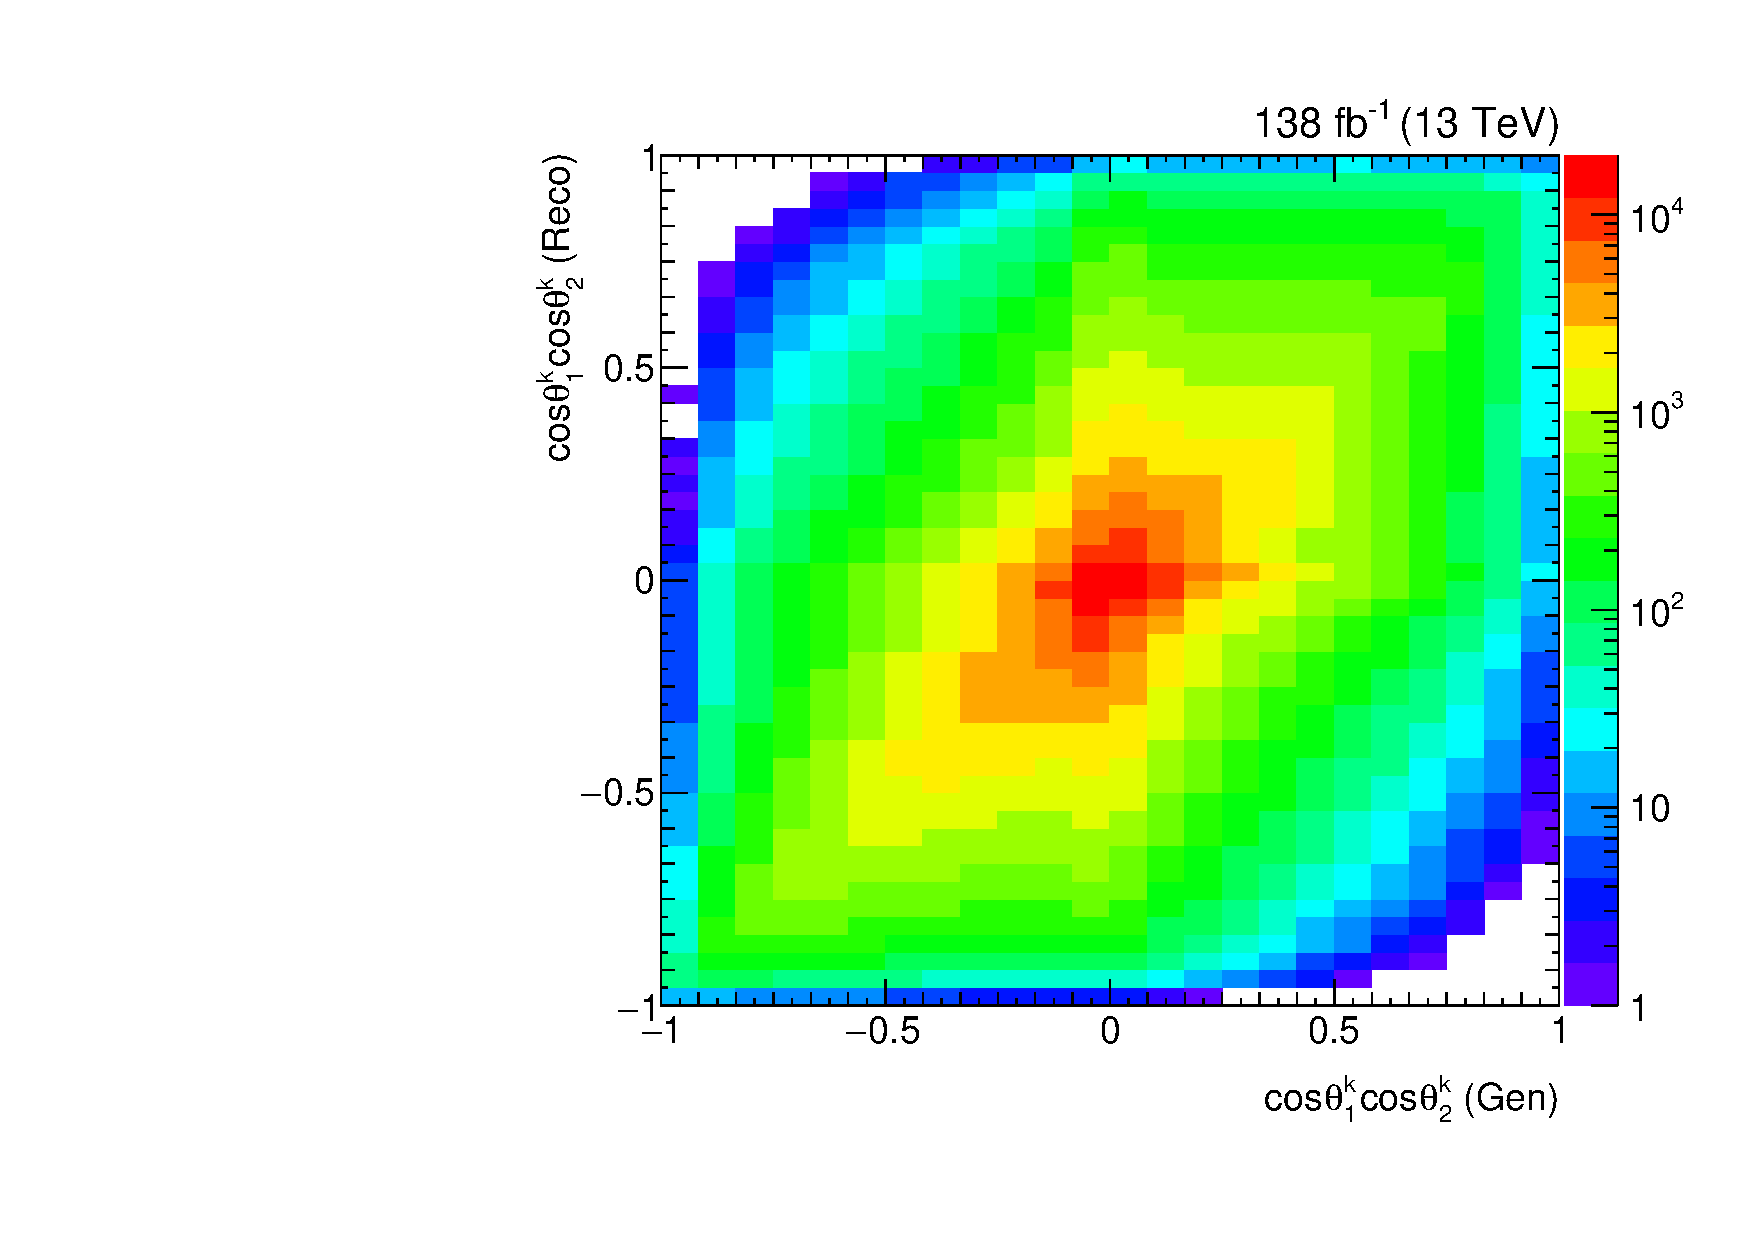
\includegraphics[width=0.40\textwidth]{fig_fullRun2UL/unfolding/combined/ResponseMatrix_c_kk.pdf} \\
 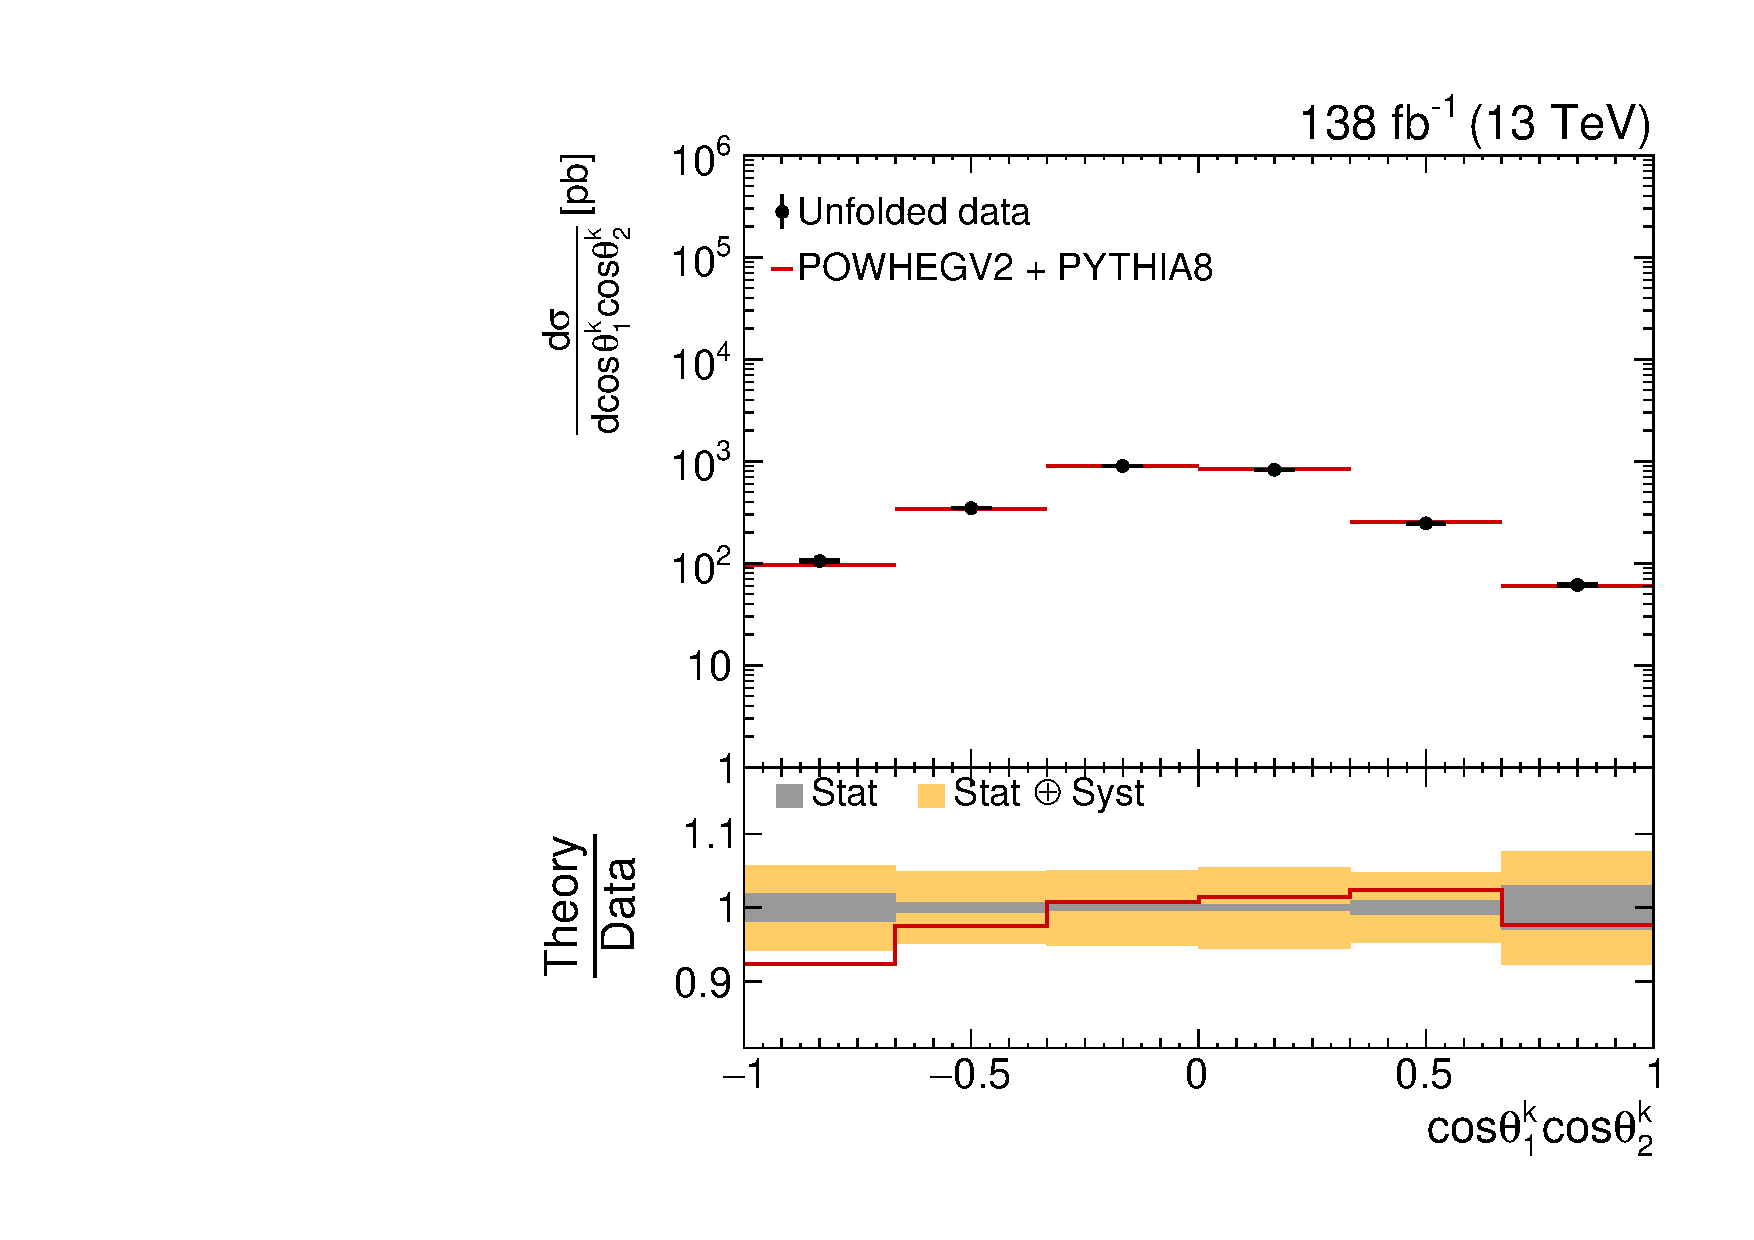
\includegraphics[width=0.40\textwidth]{fig_fullRun2UL/unfolding/combined/UnfoldedResults_c_kk.pdf}
 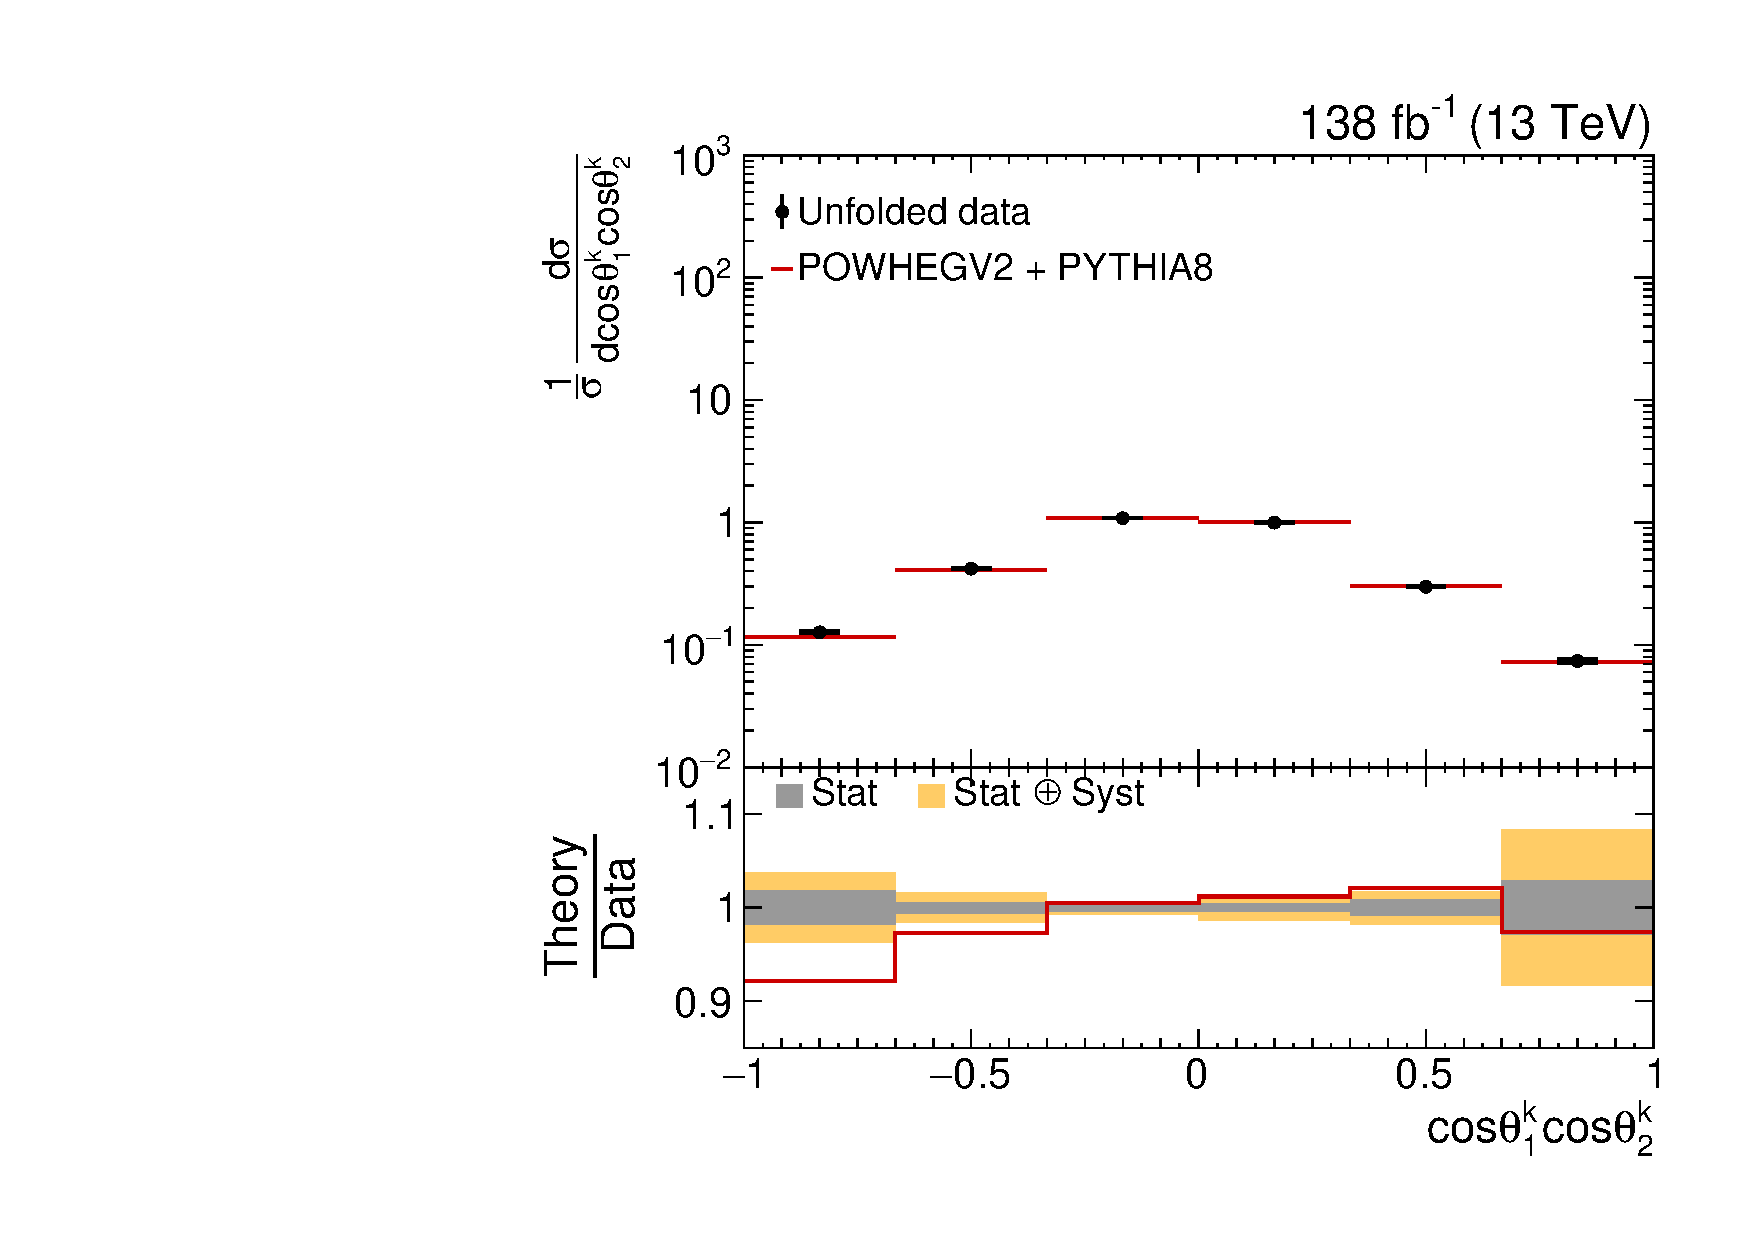
\includegraphics[width=0.40\textwidth]{fig_fullRun2UL/unfolding/combined/UnfoldedResultsNorm_c_kk.pdf} \\
\label{fig:c_kk}
\caption{Reconstructed detector-level distribution (Top Left), detector response-matrix (Top Right), absolute cross-section unfolded to parton-level (Bottom Left), and normalized cross-section unfolded to parton-level (Bottom Right) for diagonal spin correlation observable $\cos\theta_{1}^{k}\cos\theta_{2}^{k}$, from which spin-density coefficient $C_{kk}$ (sensitive to spin-density coefficient function $c_{k k}$) is extracted.}
\end{center}
\end{figure}
\clearpage
\begin{figure}[htb]
\begin{center}
 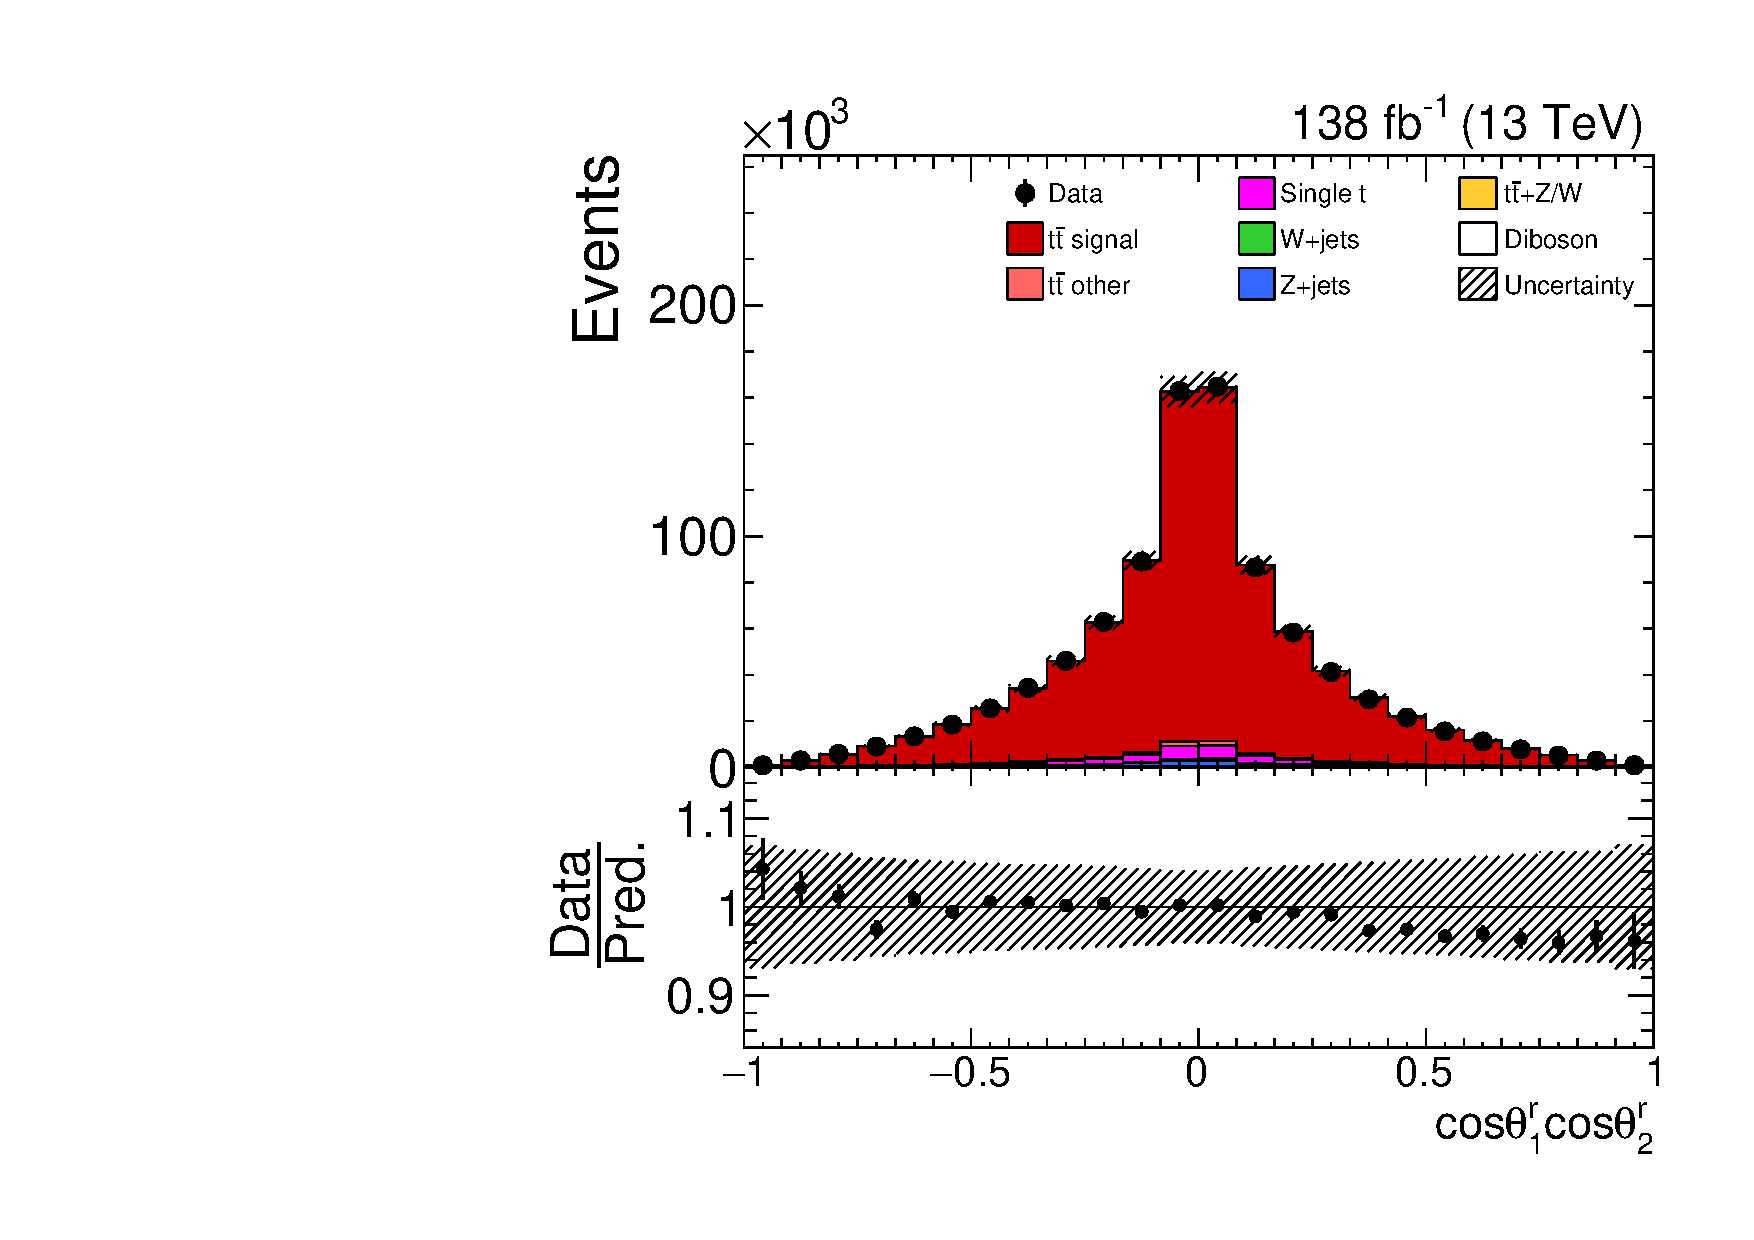
\includegraphics[width=0.40\textwidth]{fig_fullRun2UL/controlplots/combined/Hyp_LLBarCrr.pdf}
 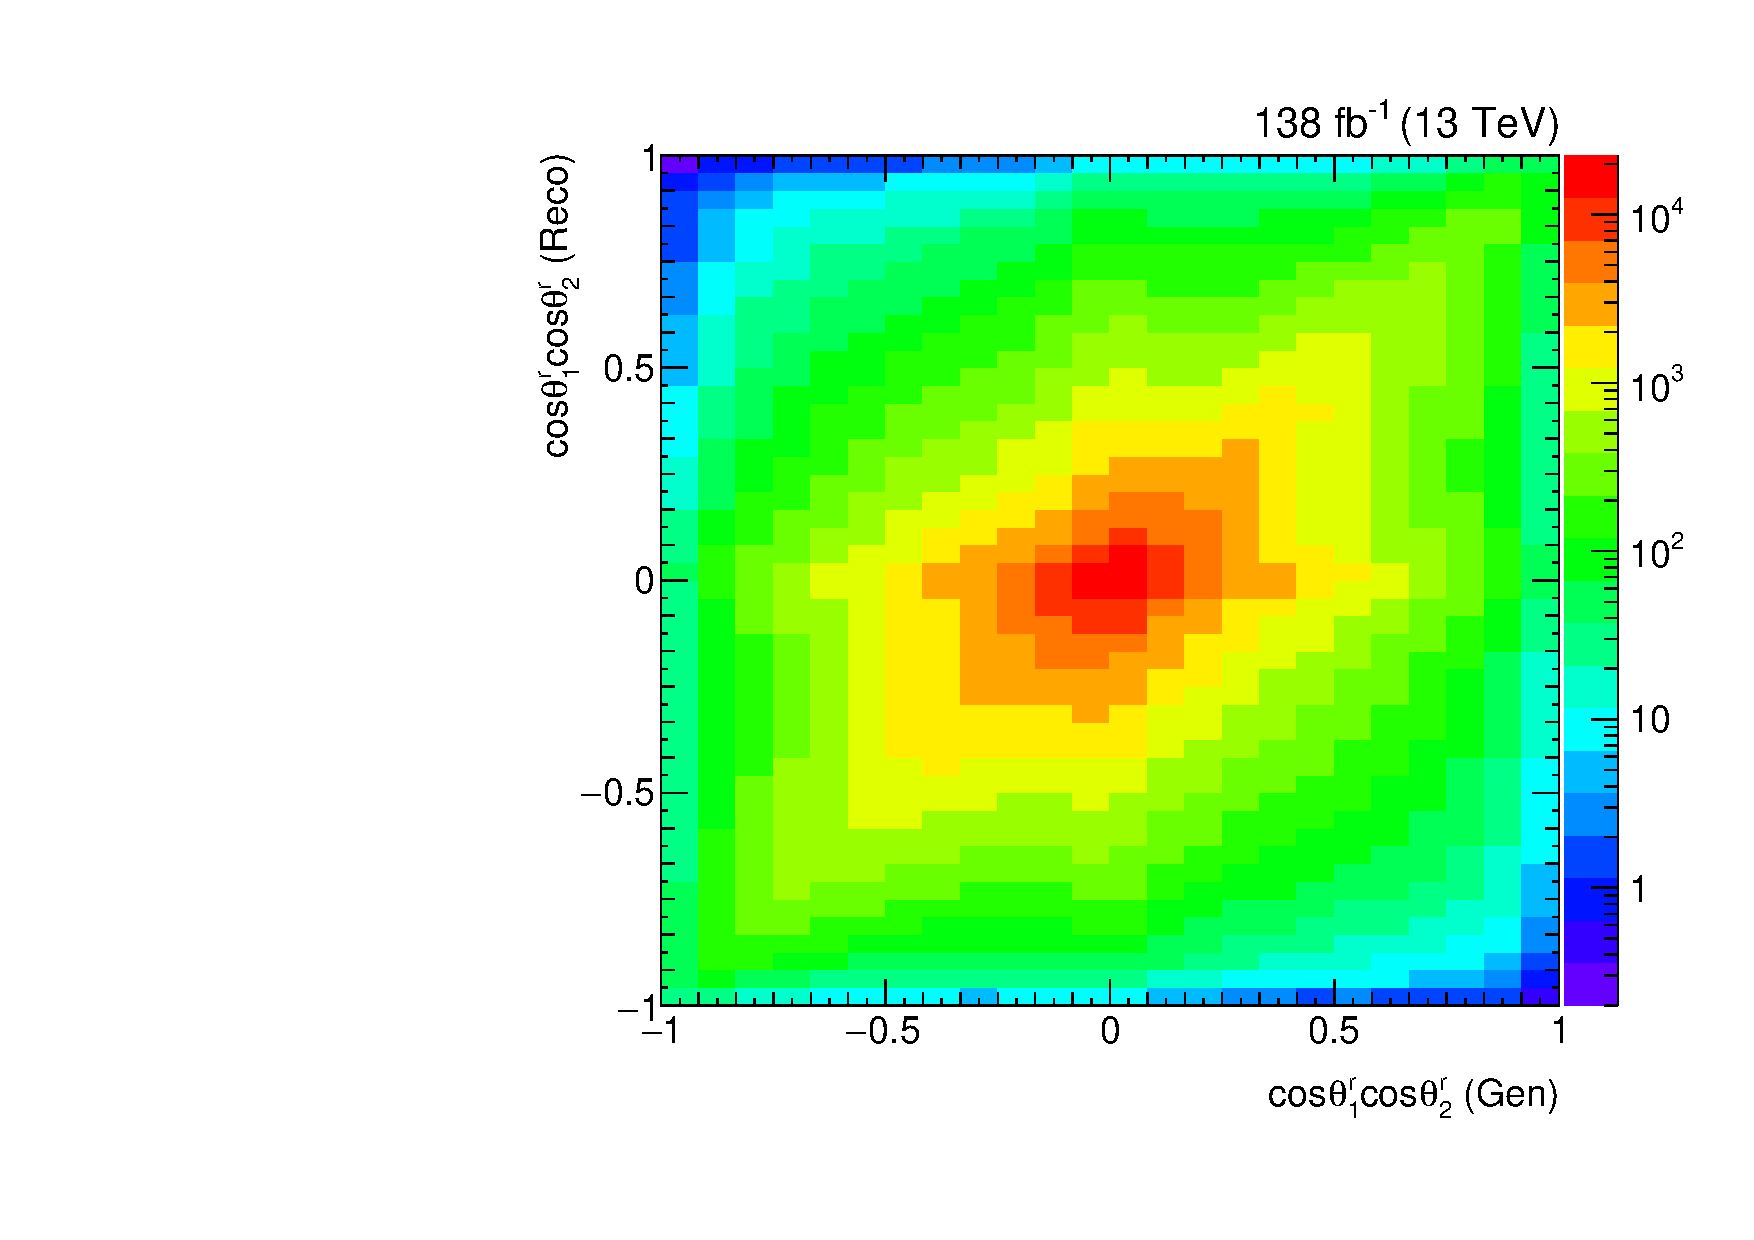
\includegraphics[width=0.40\textwidth]{fig_fullRun2UL/unfolding/combined/ResponseMatrix_c_rr.pdf} \\
 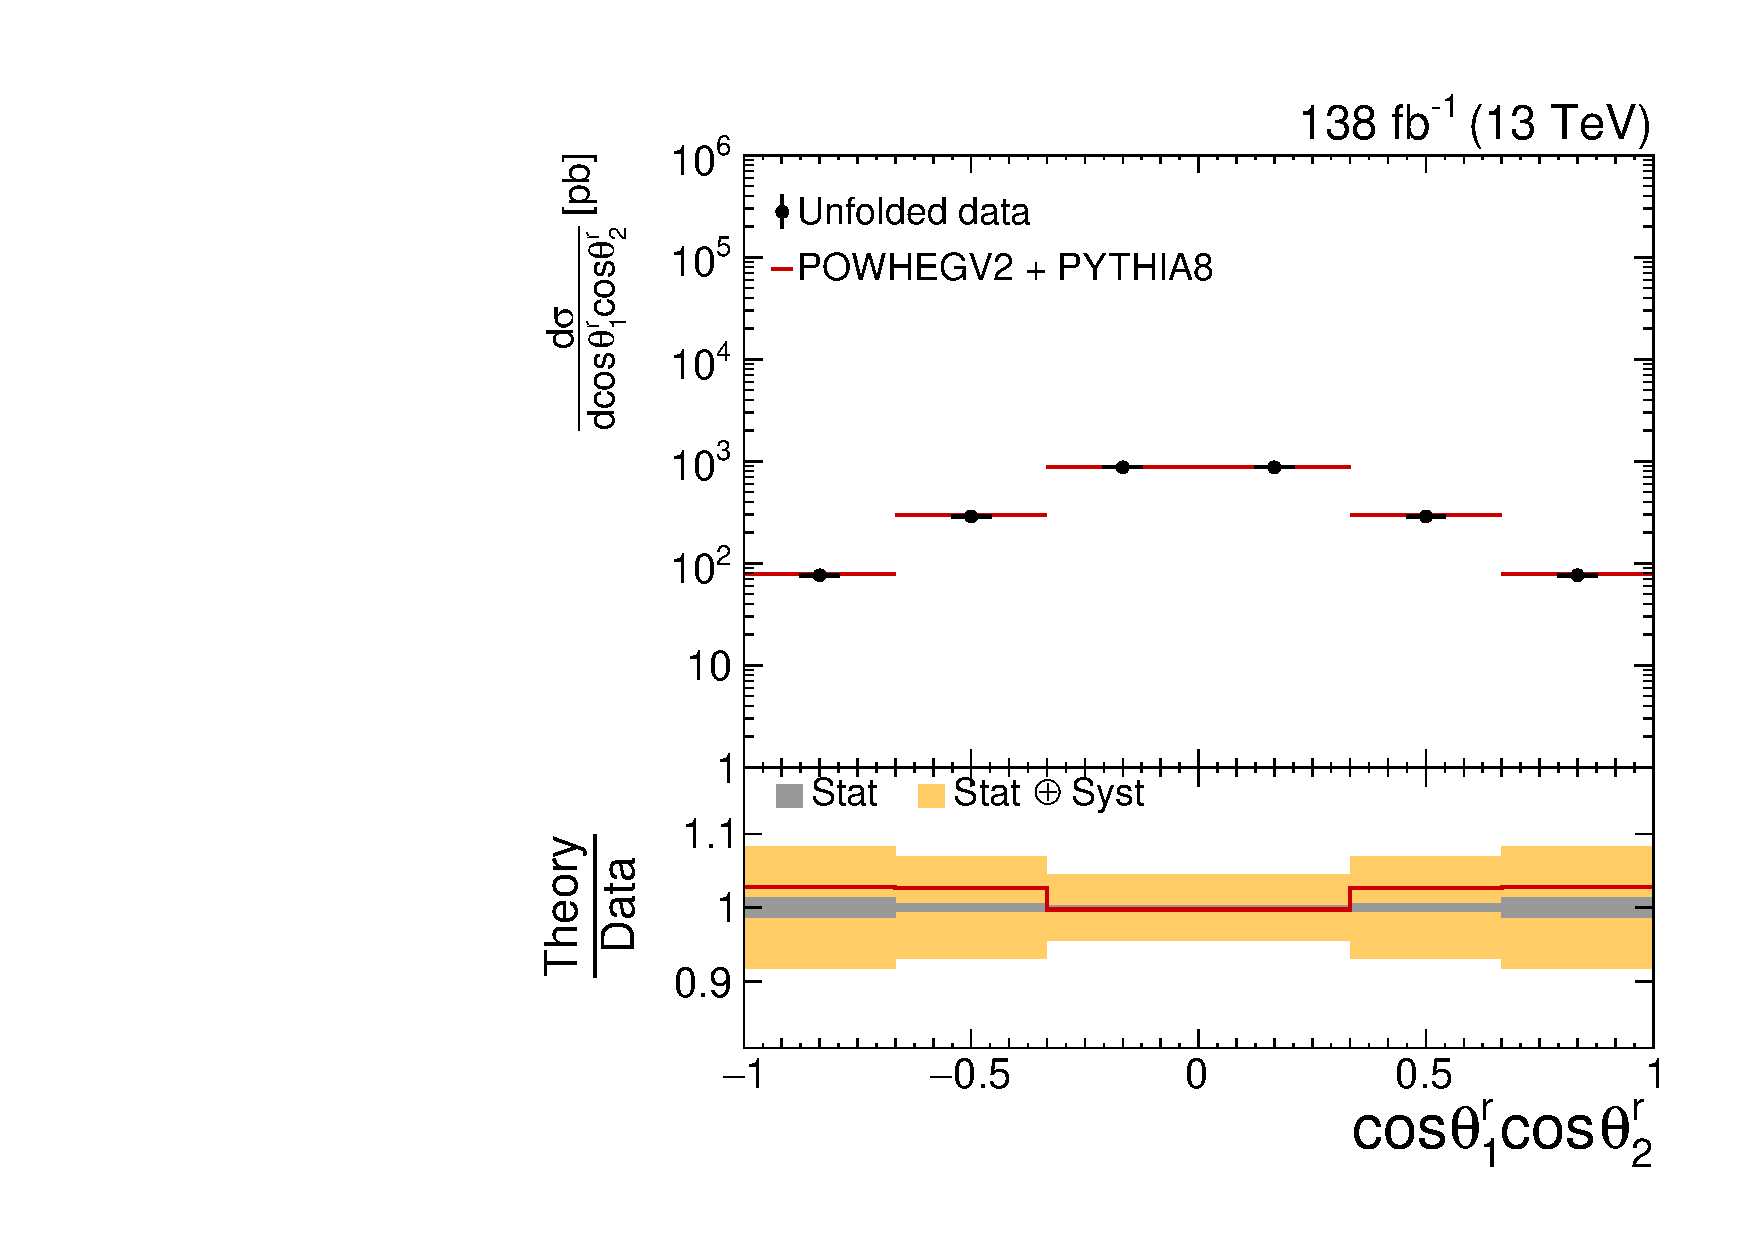
\includegraphics[width=0.40\textwidth]{fig_fullRun2UL/unfolding/combined/UnfoldedResults_c_rr.pdf}
 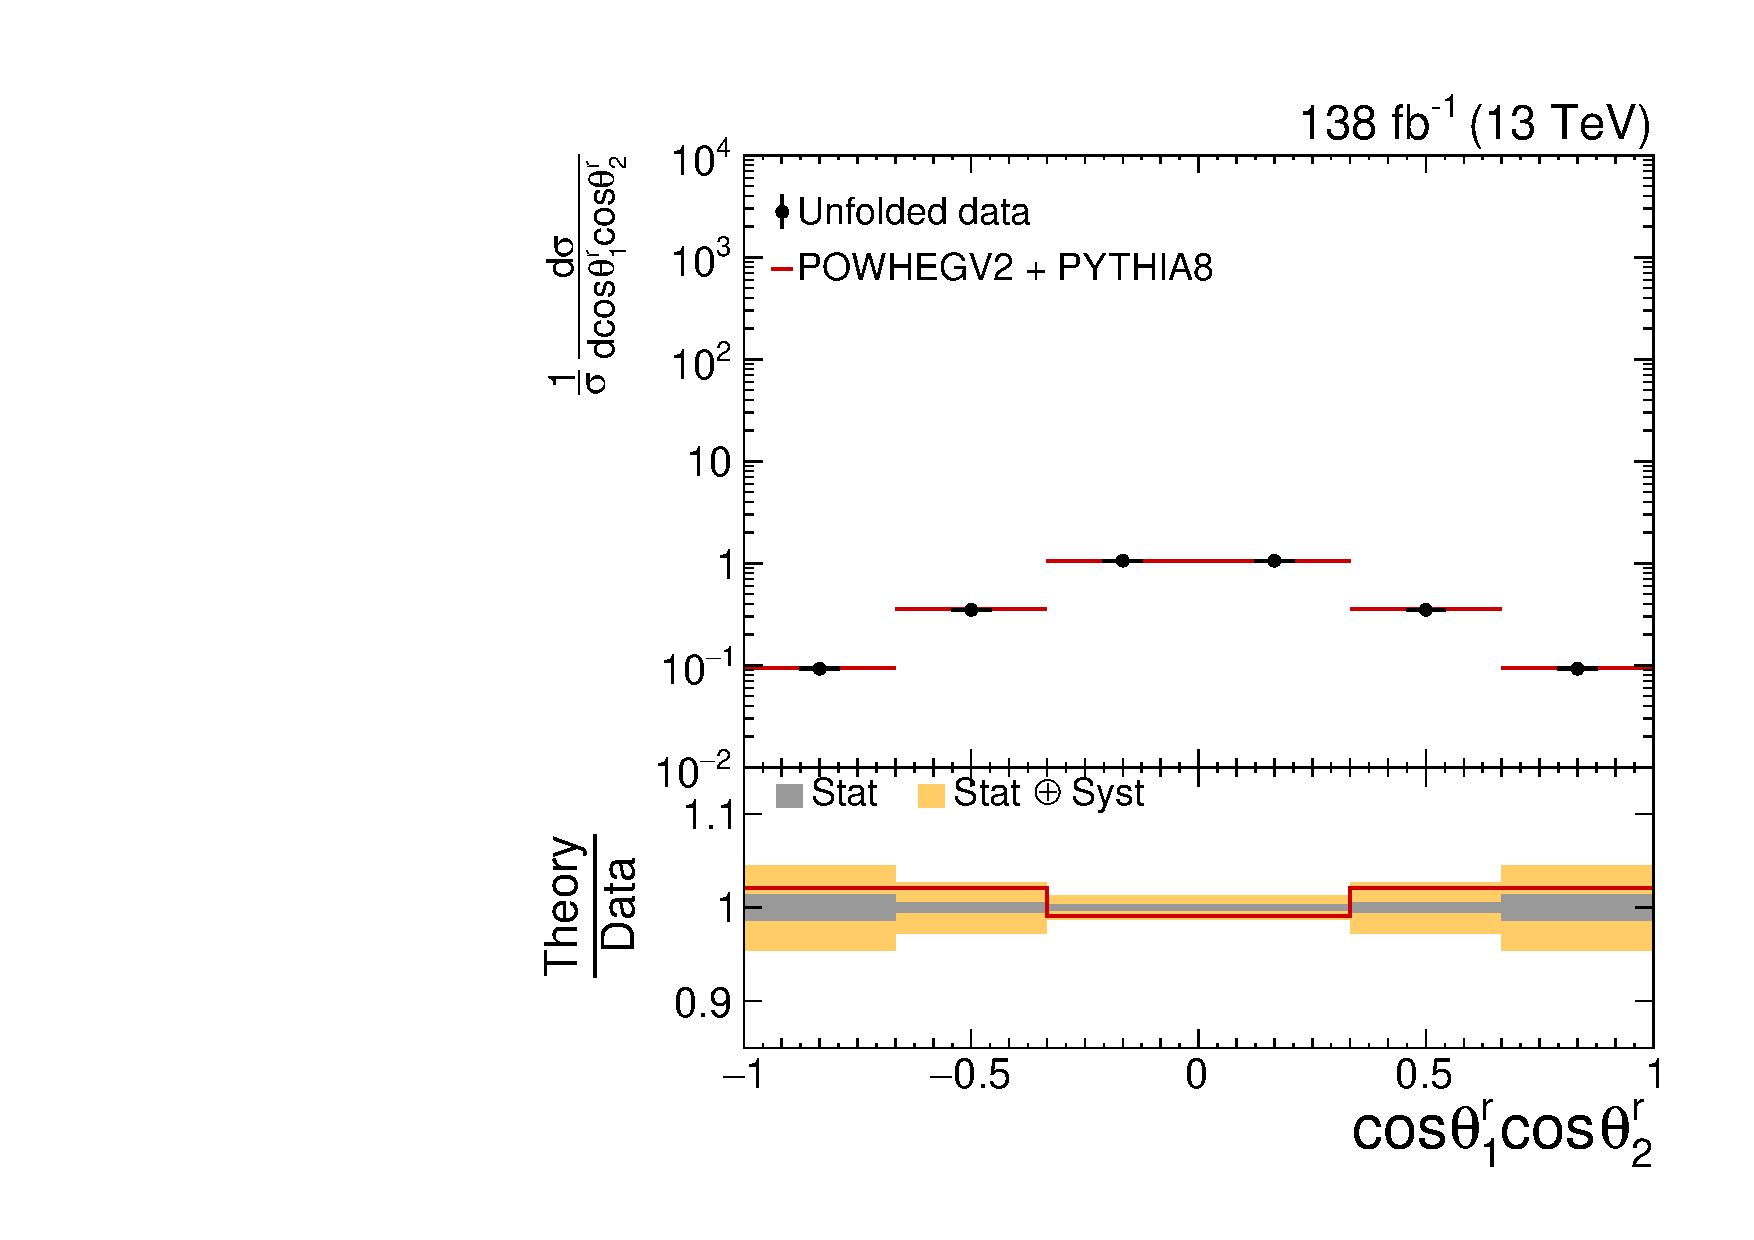
\includegraphics[width=0.40\textwidth]{fig_fullRun2UL/unfolding/combined/UnfoldedResultsNorm_c_rr.pdf} \\
\label{fig:c_rr}
\caption{Reconstructed detector-level distribution (Top Left), detector response-matrix (Top Right), absolute cross-section unfolded to parton-level (Bottom Left), and normalized cross-section unfolded to parton-level (Bottom Right) for diagonal spin correlation observable $\cos\theta_{1}^{r}\cos\theta_{2}^{r}$, from which spin-density coefficient $C_{rr}$ (sensitive to spin-density coefficient function $c_{r r}$) is extracted.}
\end{center}
\end{figure}
\clearpage
\begin{figure}[htb]
\begin{center}
 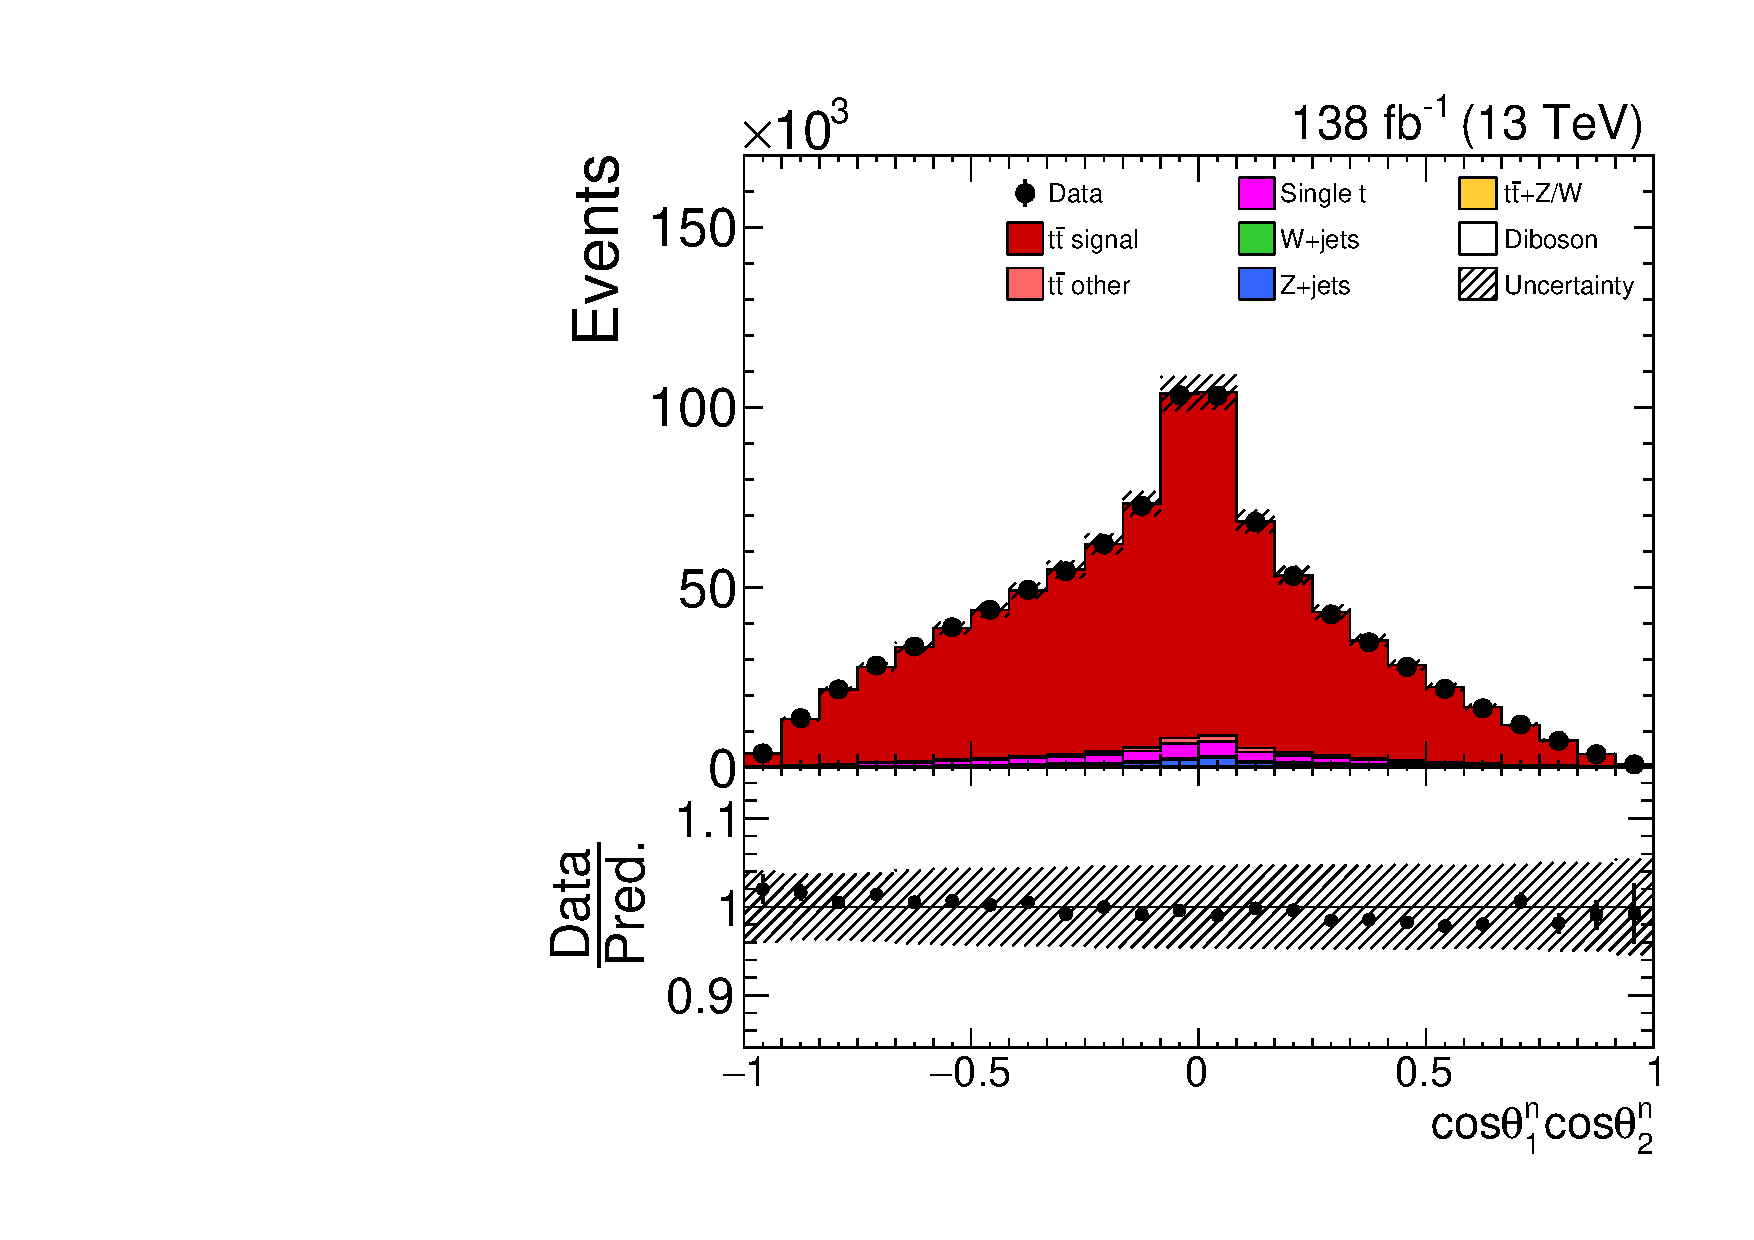
\includegraphics[width=0.40\textwidth]{fig_fullRun2UL/controlplots/combined/Hyp_LLBarCnn.pdf}
 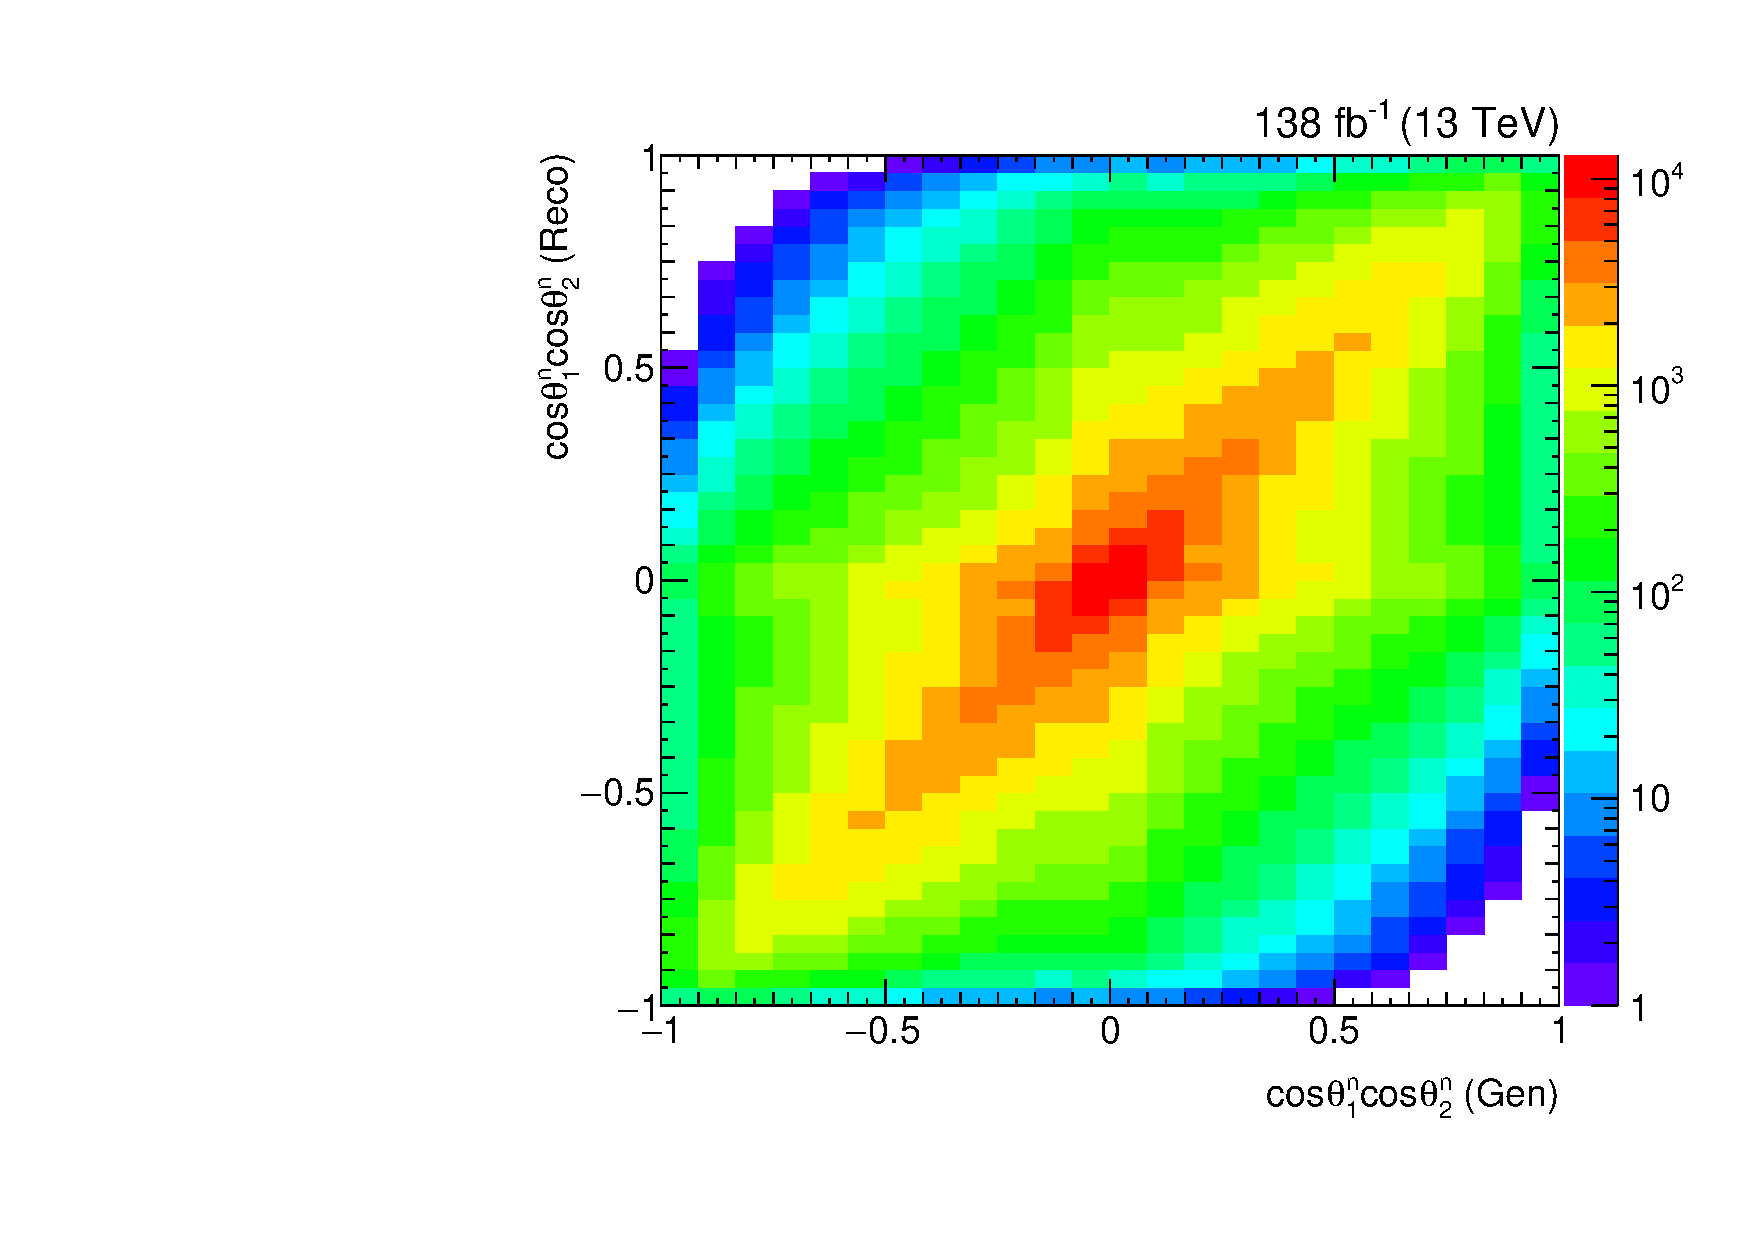
\includegraphics[width=0.40\textwidth]{fig_fullRun2UL/unfolding/combined/ResponseMatrix_c_nn.pdf} \\
 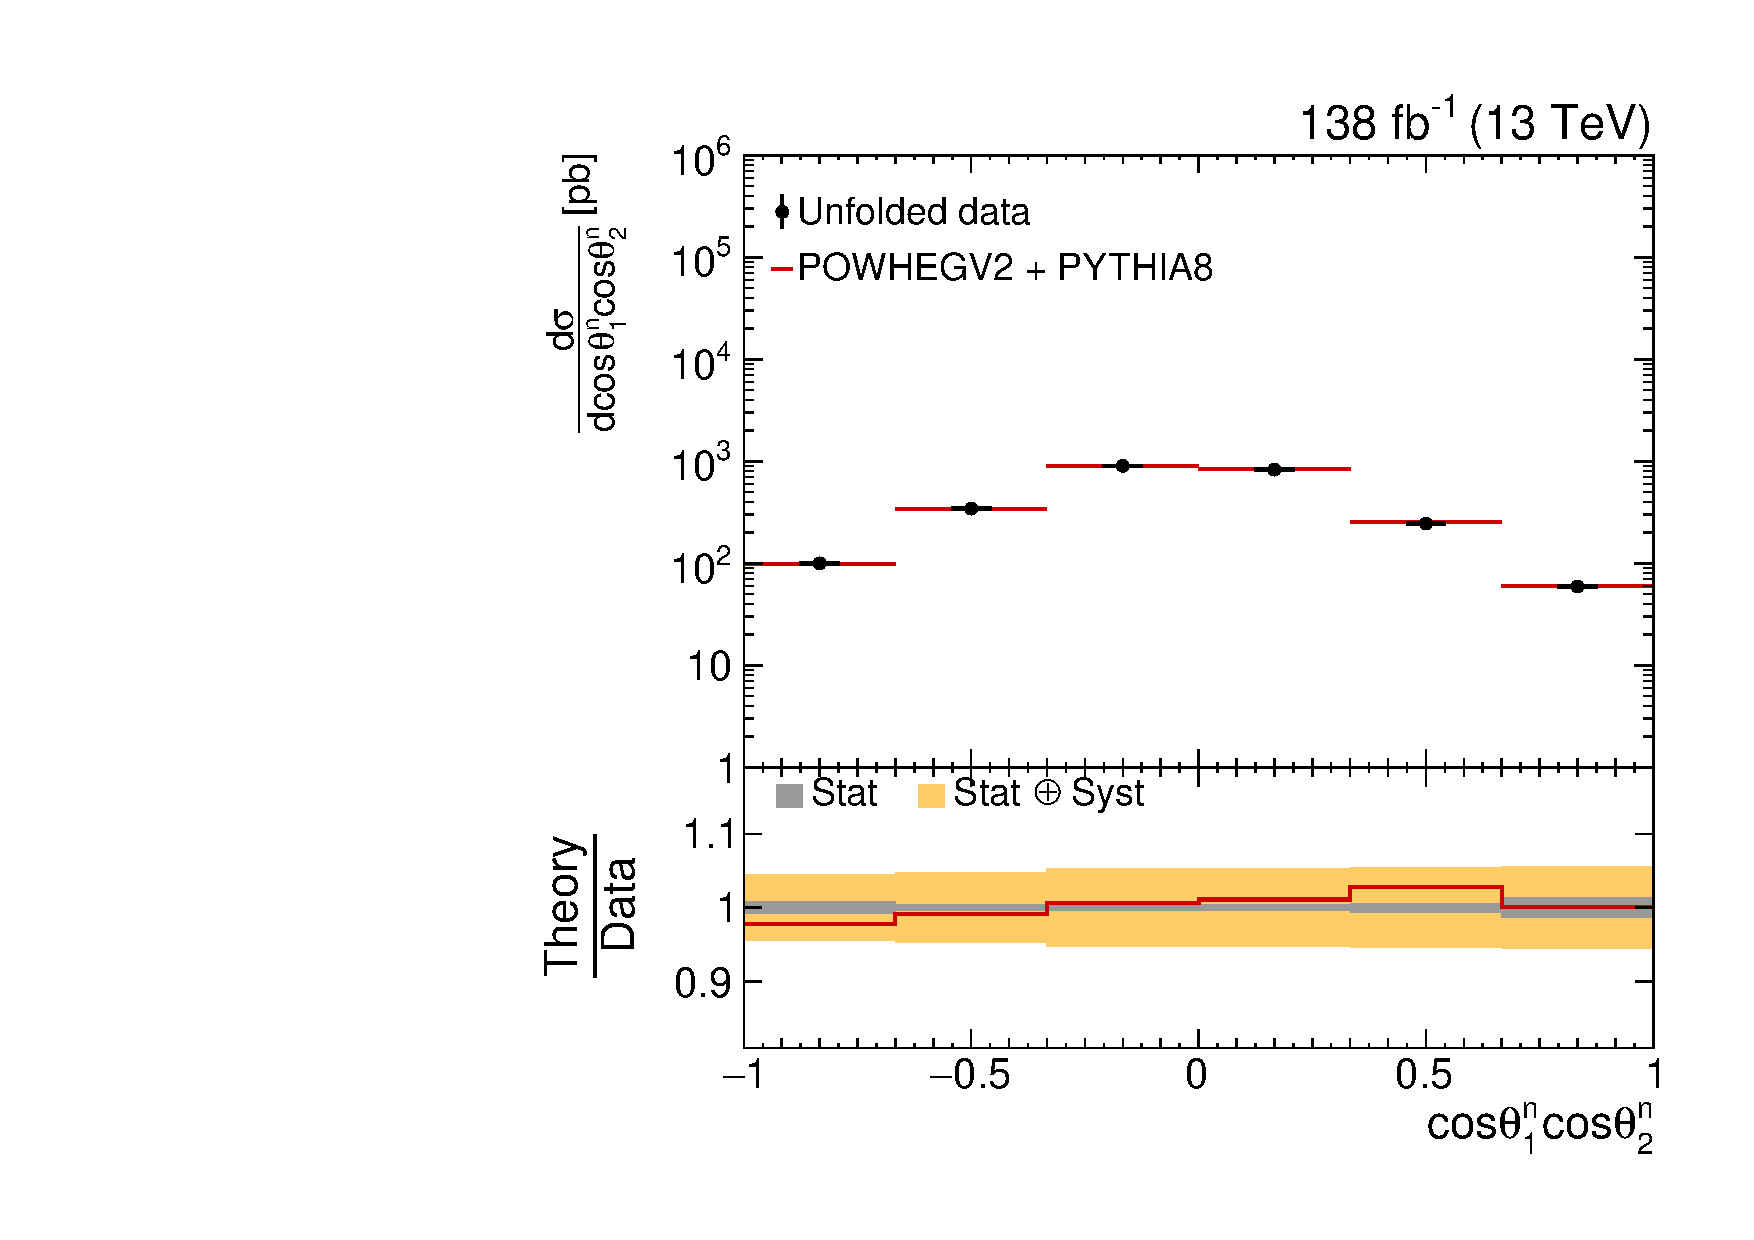
\includegraphics[width=0.40\textwidth]{fig_fullRun2UL/unfolding/combined/UnfoldedResults_c_nn.pdf}
 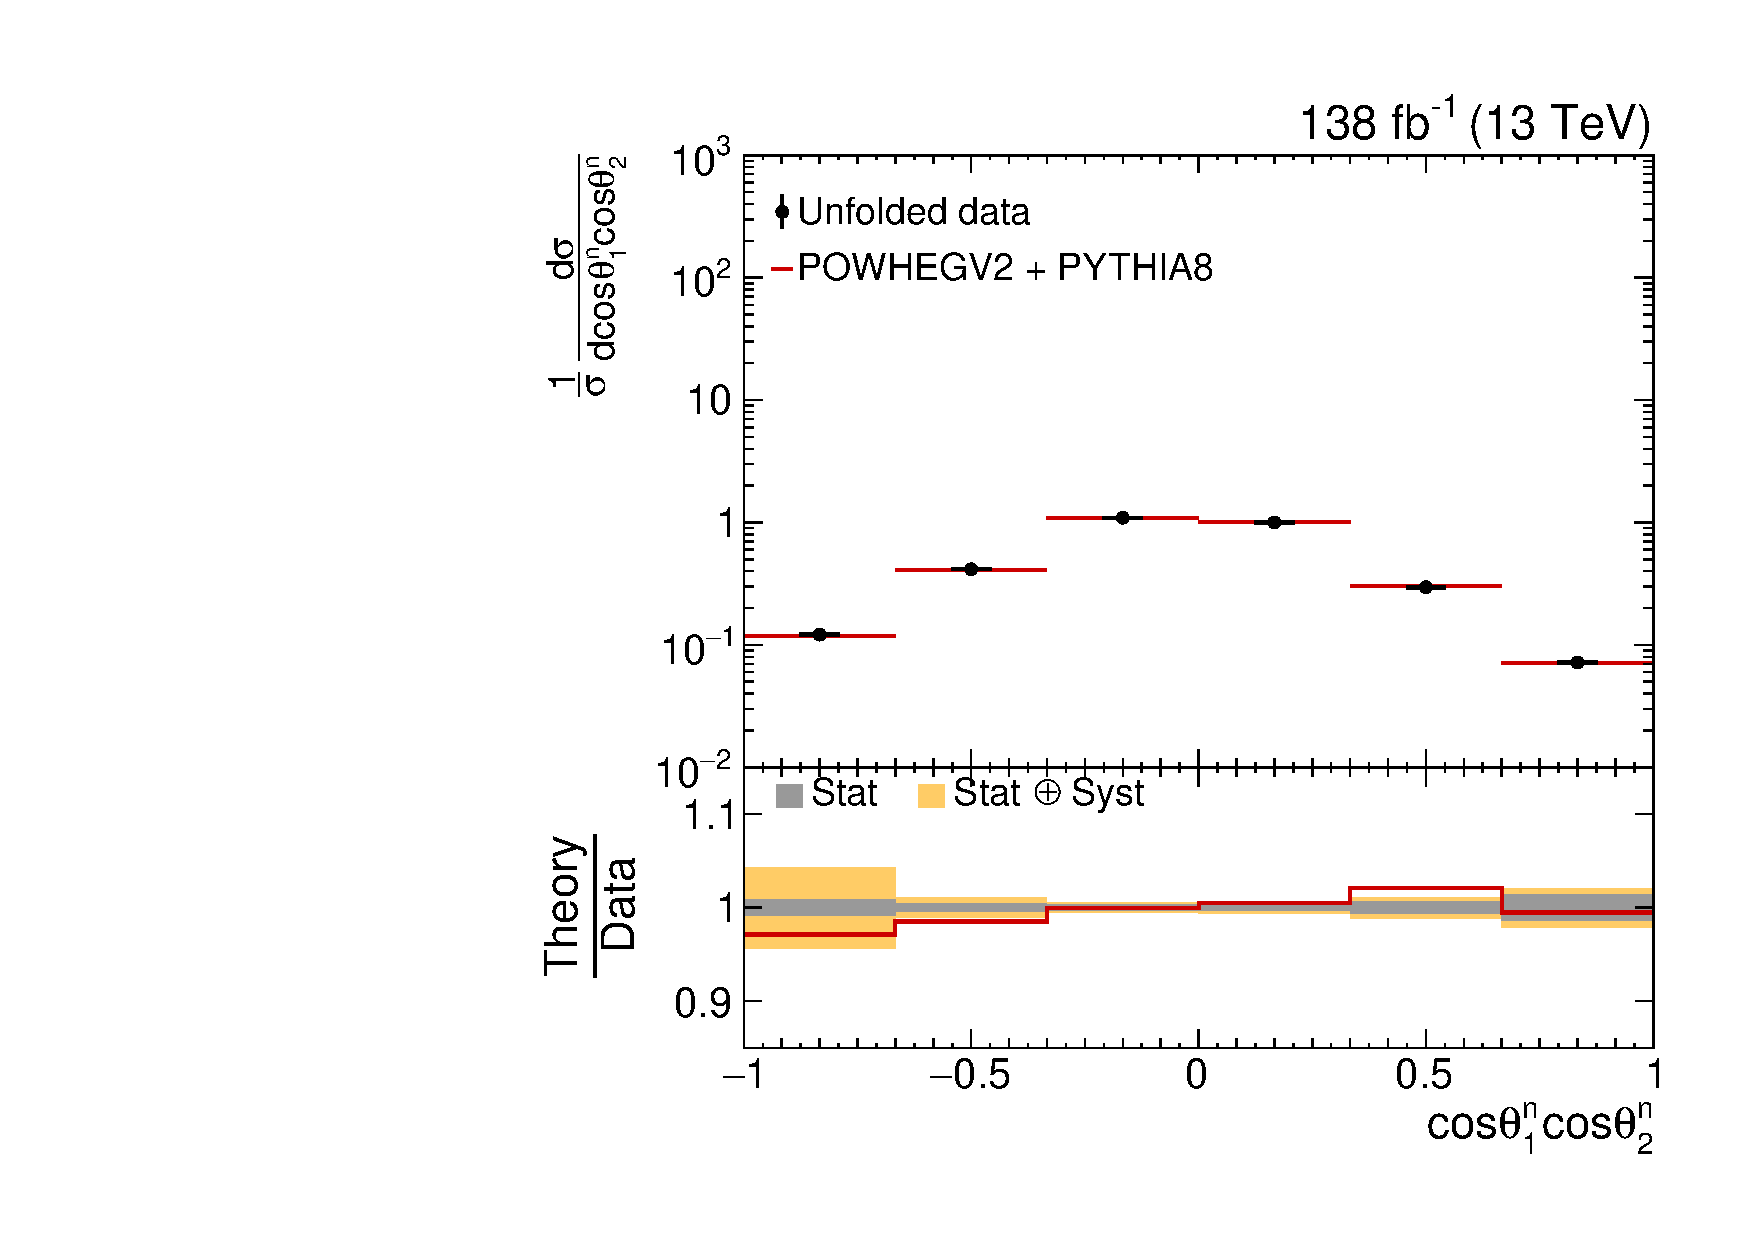
\includegraphics[width=0.40\textwidth]{fig_fullRun2UL/unfolding/combined/UnfoldedResultsNorm_c_nn.pdf} \\
\label{fig:c_nn}
\caption{Reconstructed detector-level distribution (Top Left), detector response-matrix (Top Right), absolute cross-section unfolded to parton-level (Bottom Left), and normalized cross-section unfolded to parton-level (Bottom Right) for diagonal spin correlation observable $\cos\theta_{1}^{n}\cos\theta_{2}^{n}$, from which spin-density coefficient $C_{nn}$ (sensitive to spin-density coefficient function $c_{n n}$) is extracted.}
\end{center}
\end{figure}
\clearpage
\begin{figure}[htb]
\begin{center}
 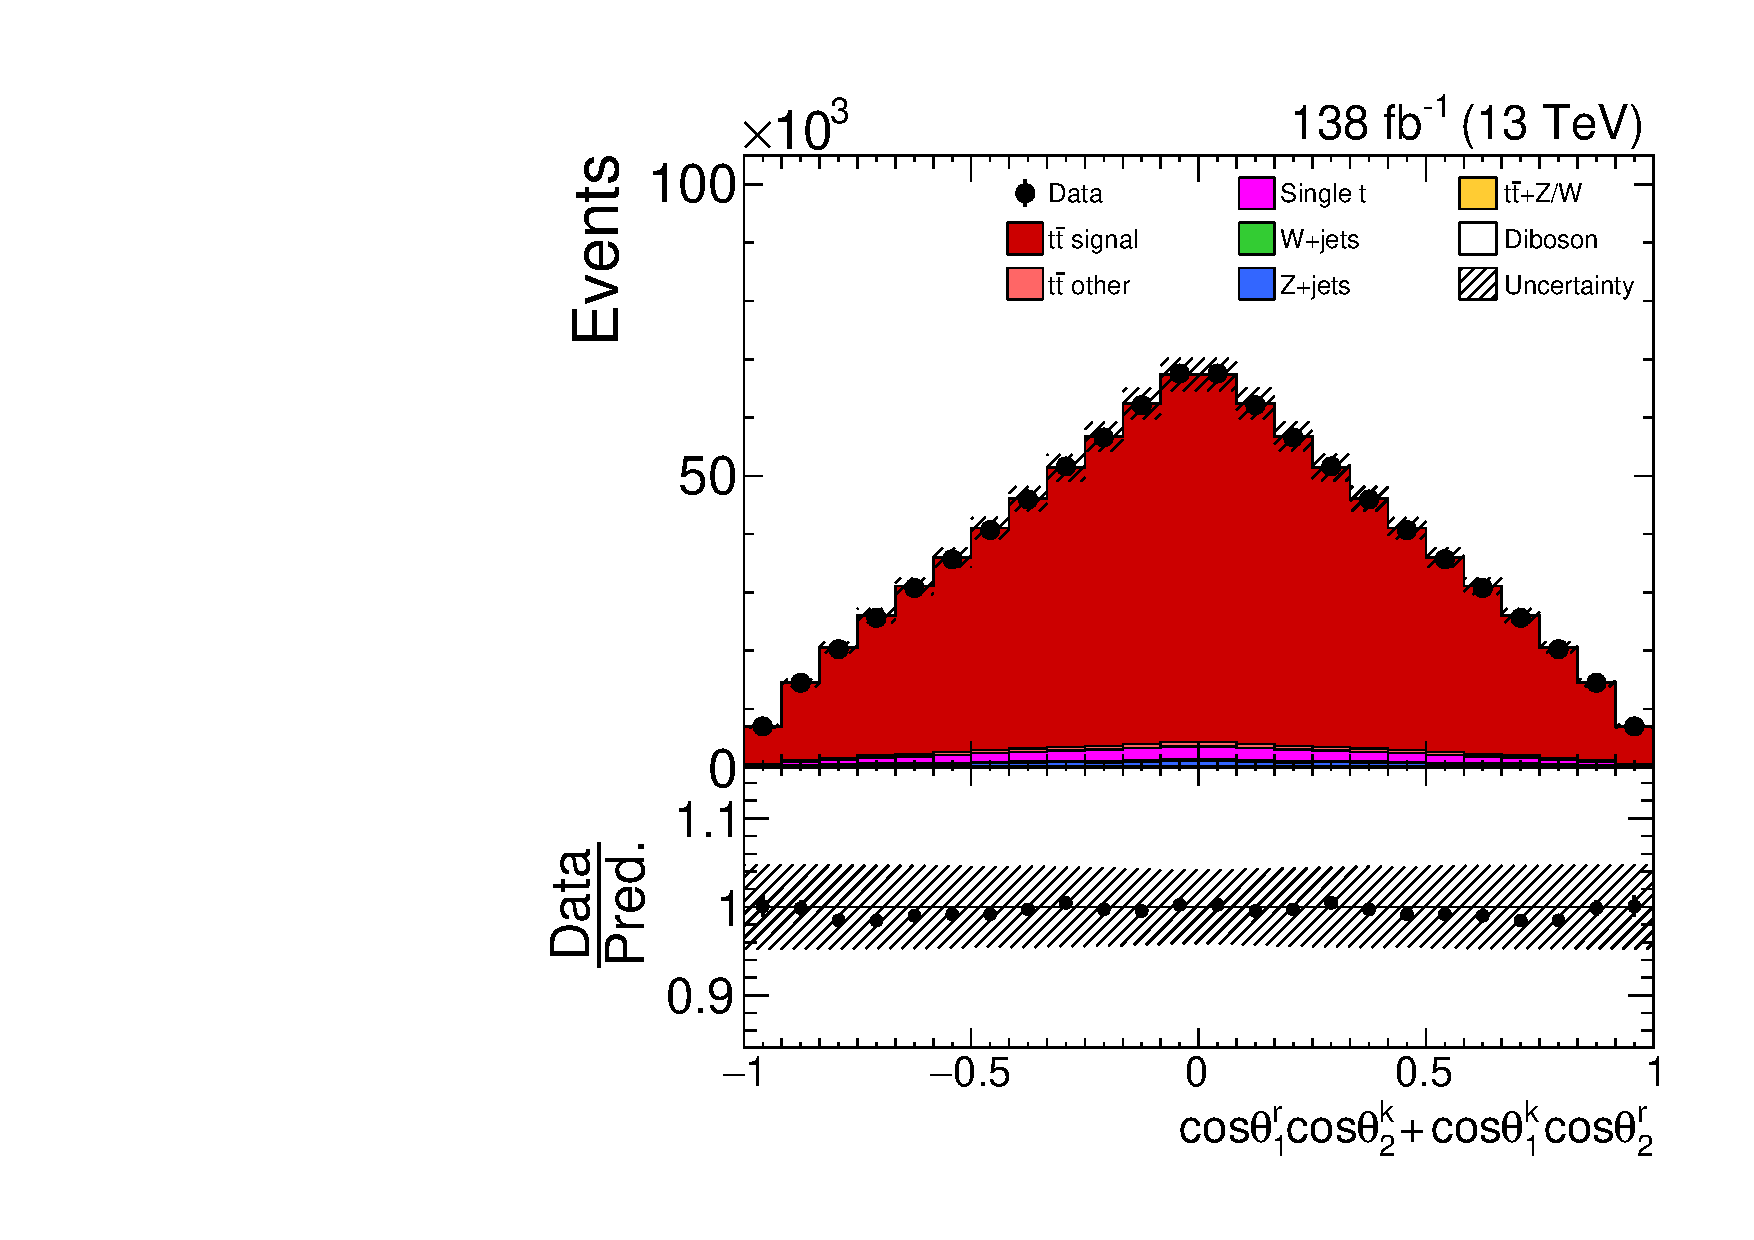
\includegraphics[width=0.40\textwidth]{fig_fullRun2UL/controlplots/combined/Hyp_LLBarCPrk.pdf}
 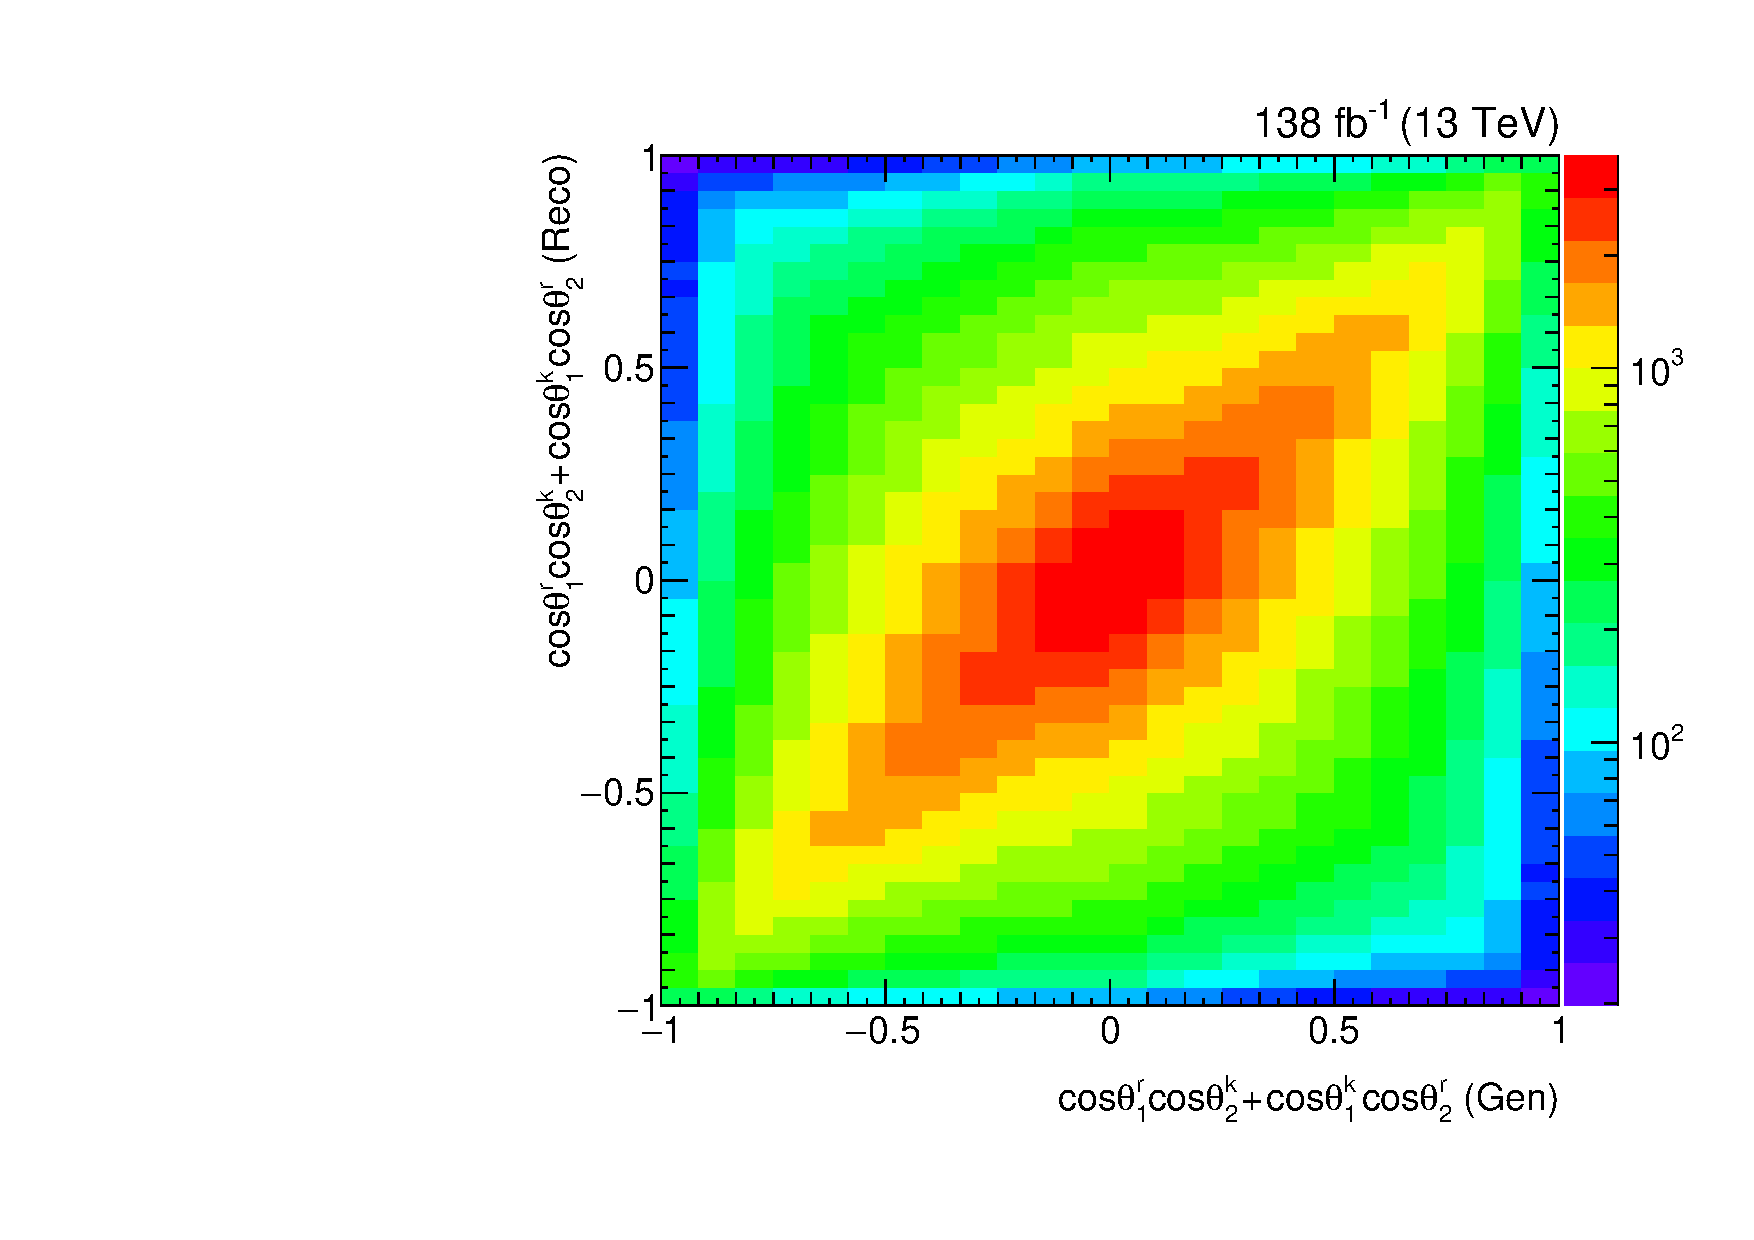
\includegraphics[width=0.40\textwidth]{fig_fullRun2UL/unfolding/combined/ResponseMatrix_c_Prk.pdf} \\
 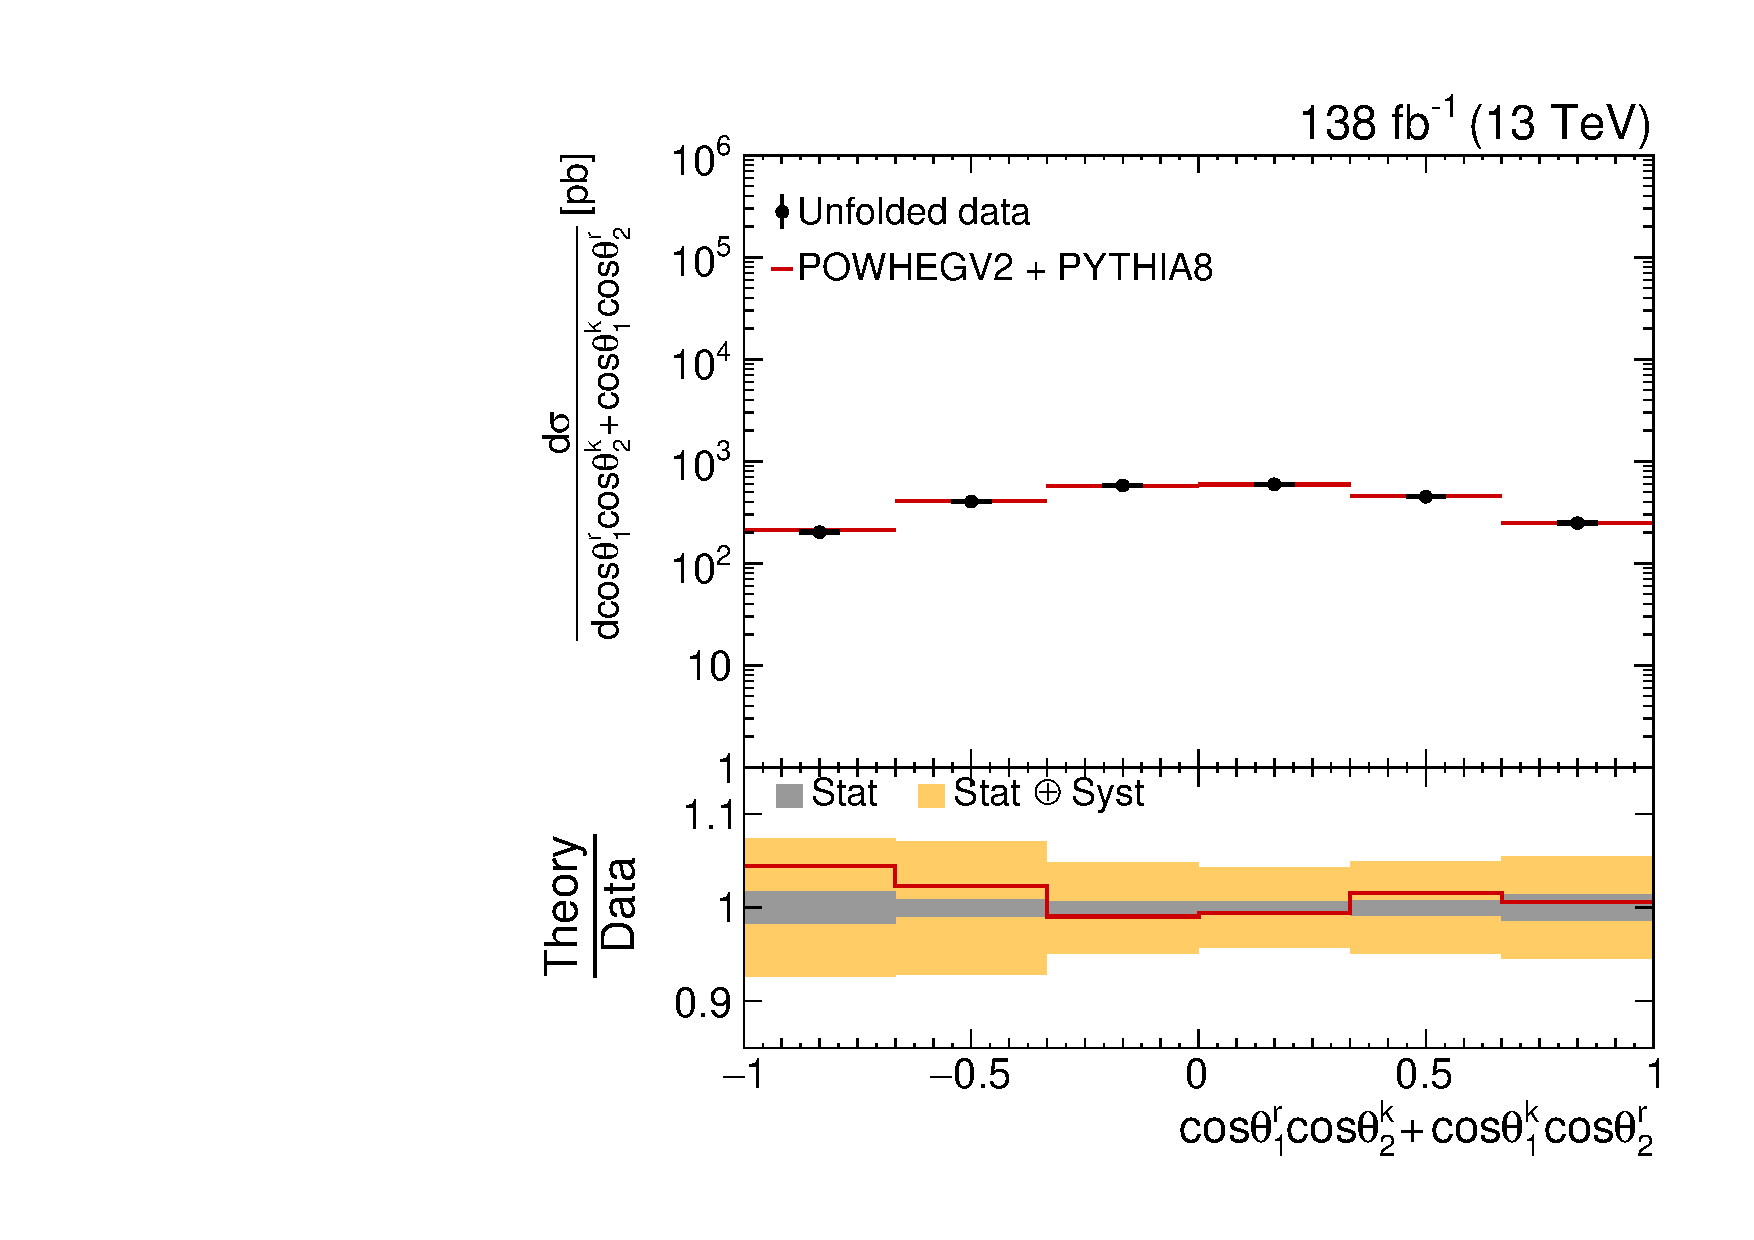
\includegraphics[width=0.40\textwidth]{fig_fullRun2UL/unfolding/combined/UnfoldedResults_c_Prk.pdf}
 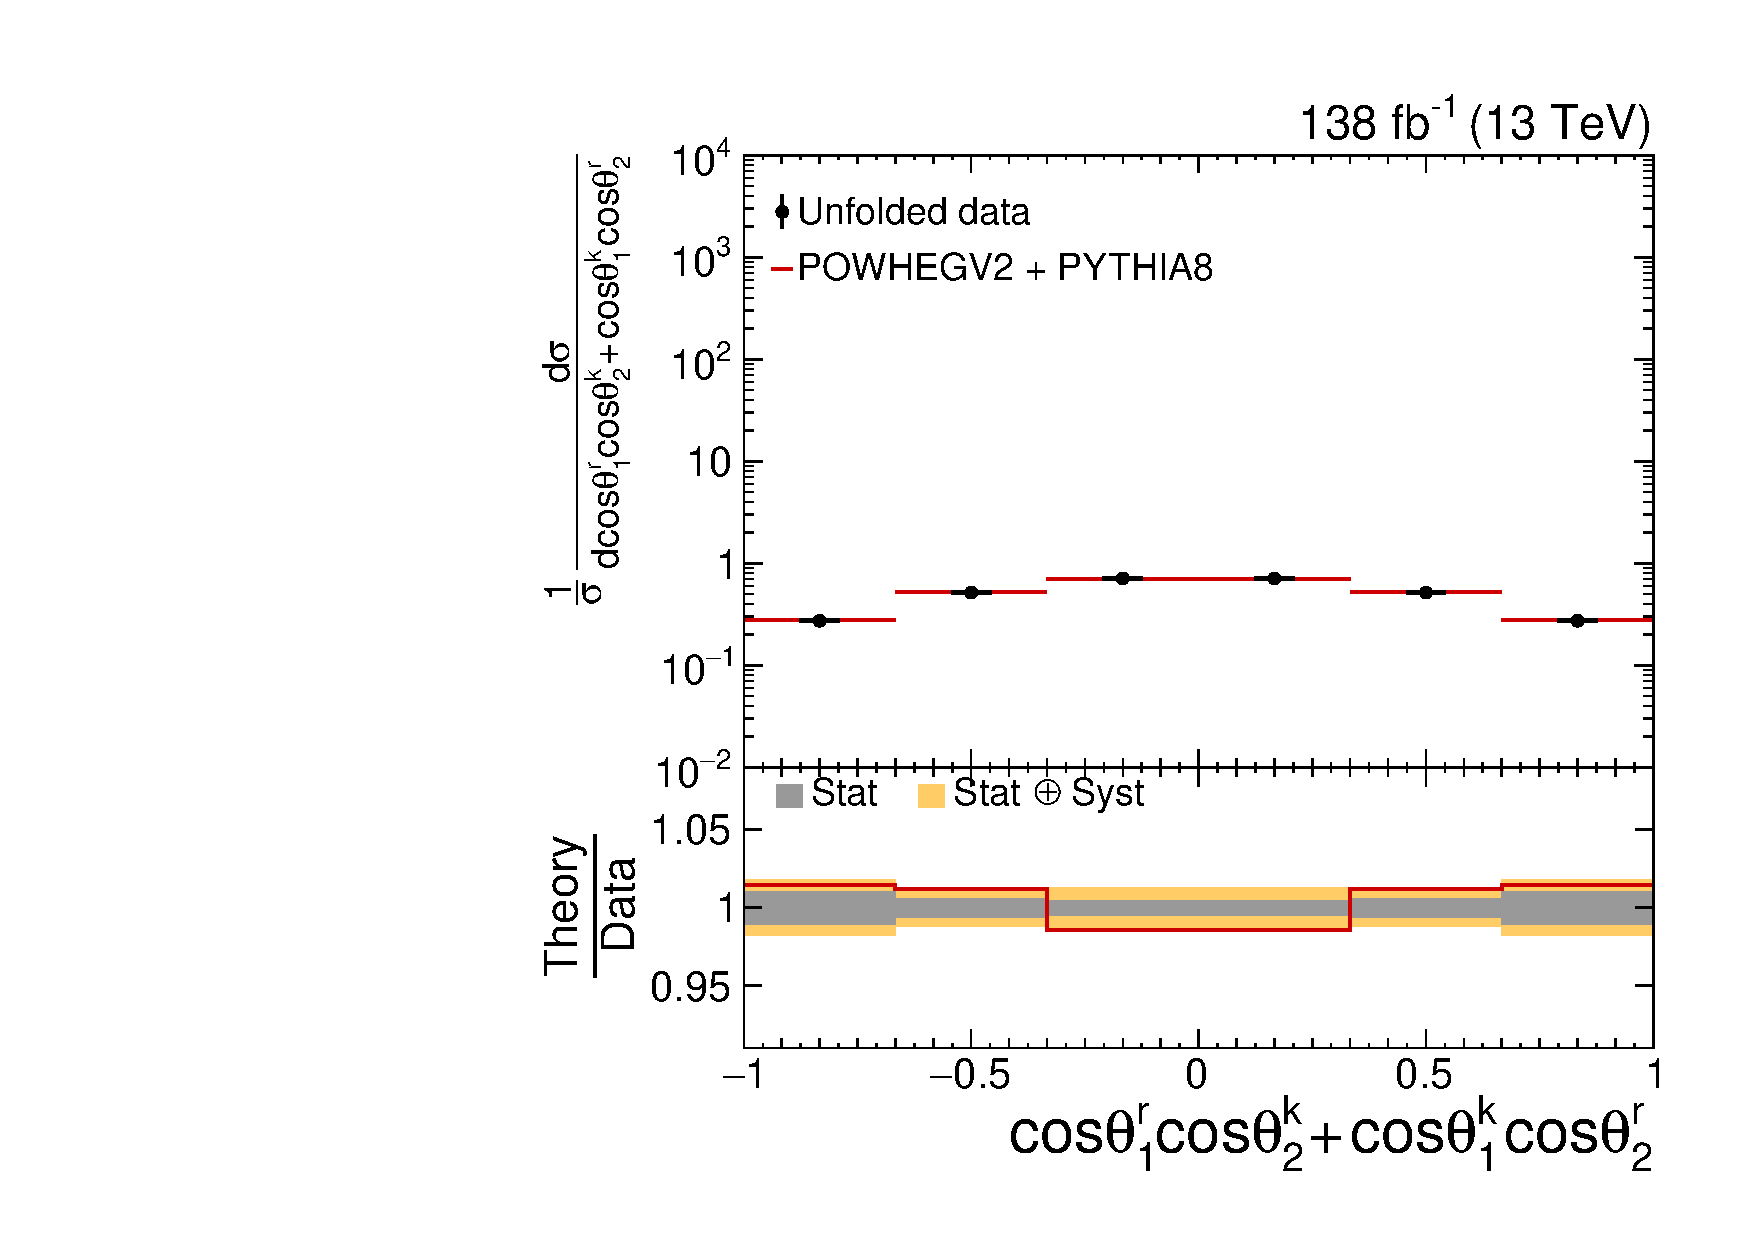
\includegraphics[width=0.40\textwidth]{fig_fullRun2UL/unfolding/combined/UnfoldedResultsNorm_c_Prk.pdf} \\
\label{fig:c_Prk}
\caption{Reconstructed detector-level distribution (Top Left), detector response-matrix (Top Right), absolute cross-section unfolded to parton-level (Bottom Left), and normalized cross-section unfolded to parton-level (Bottom Right) for off-diagonal spin correlation sum observable $\cos\theta_{1}^{r}\cos\theta_{2}^{k}+\cos\theta_{1}^{k}\cos\theta_{2}^{r}$, from which spin-density coefficient $C_{rk}+C_{kr}$ (sensitive to spin-density coefficient function $c_{r k}$) is extracted.}
\end{center}
\end{figure}
\clearpage
\begin{figure}[htb]
\begin{center}
 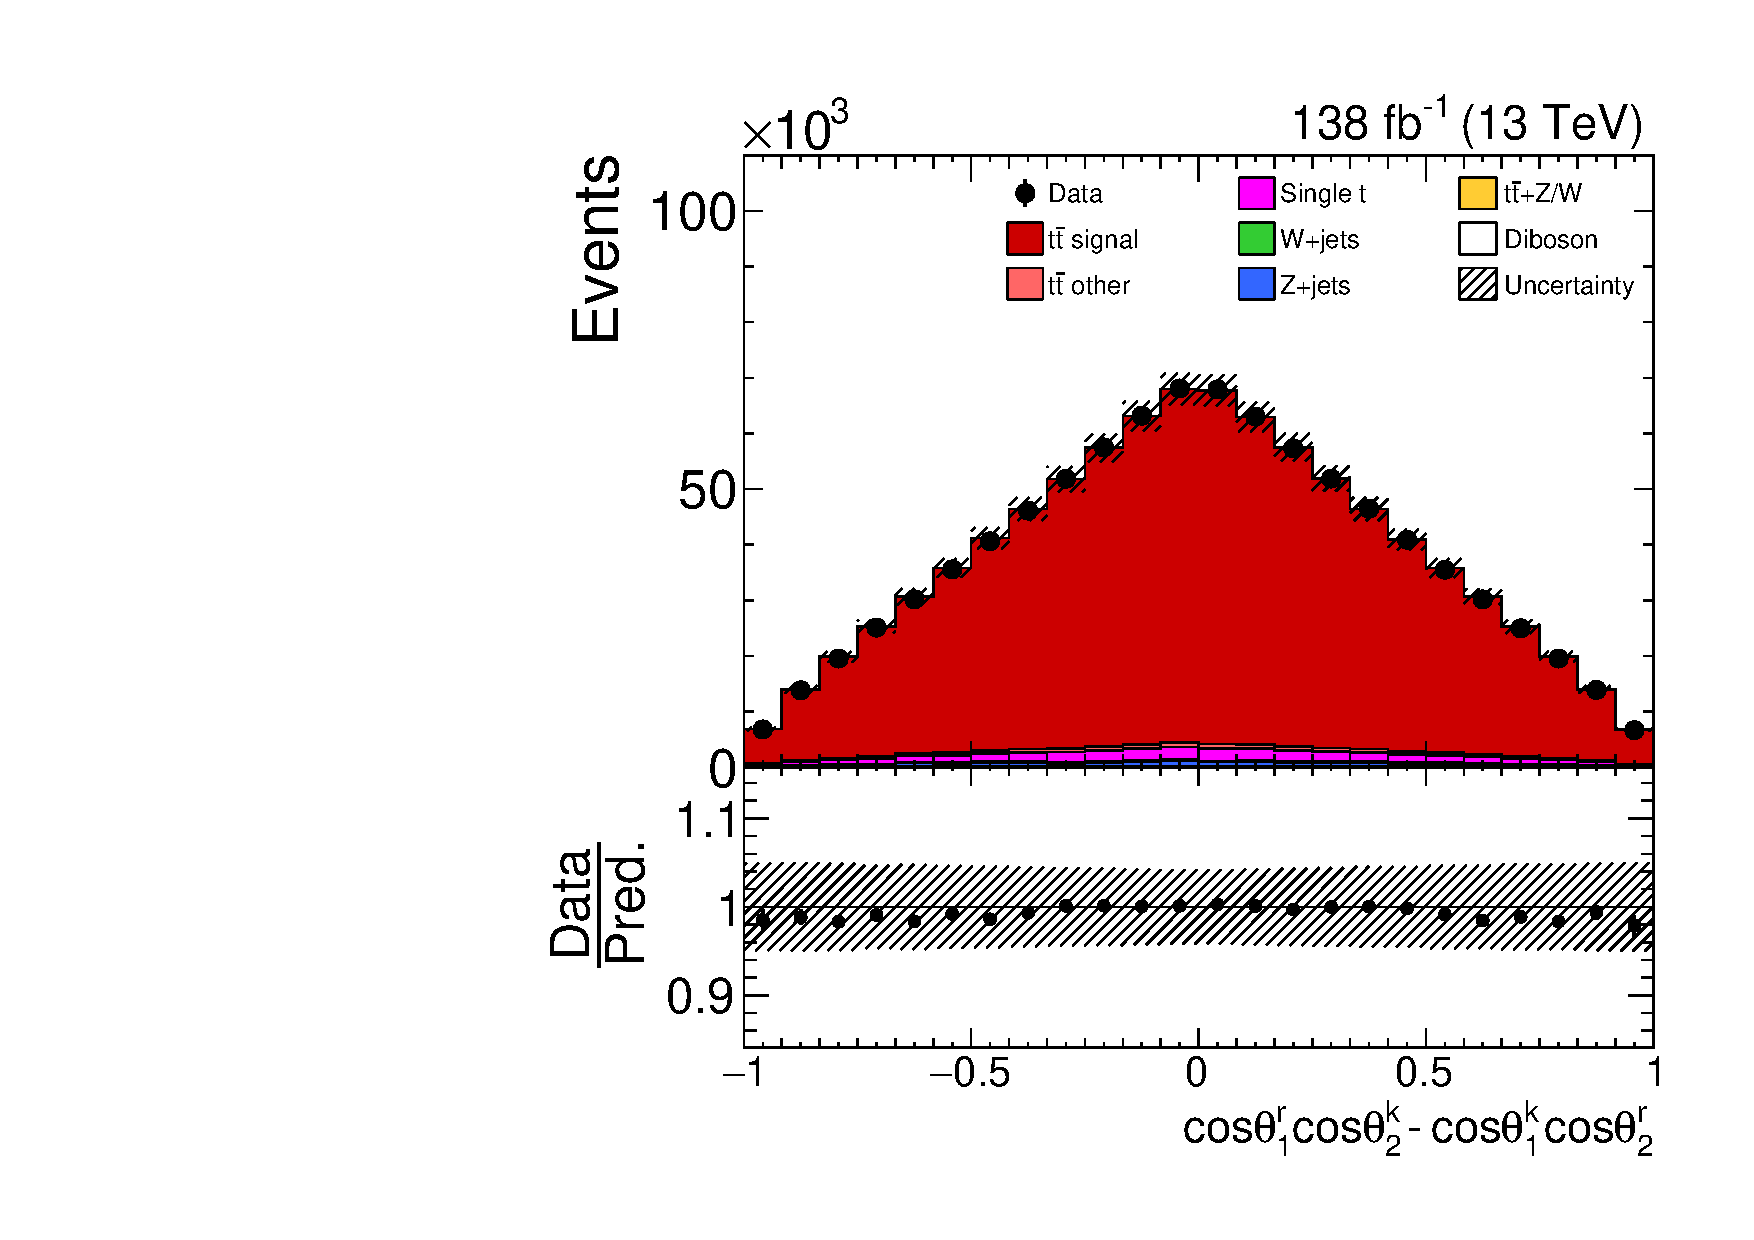
\includegraphics[width=0.40\textwidth]{fig_fullRun2UL/controlplots/combined/Hyp_LLBarCMrk.pdf}
 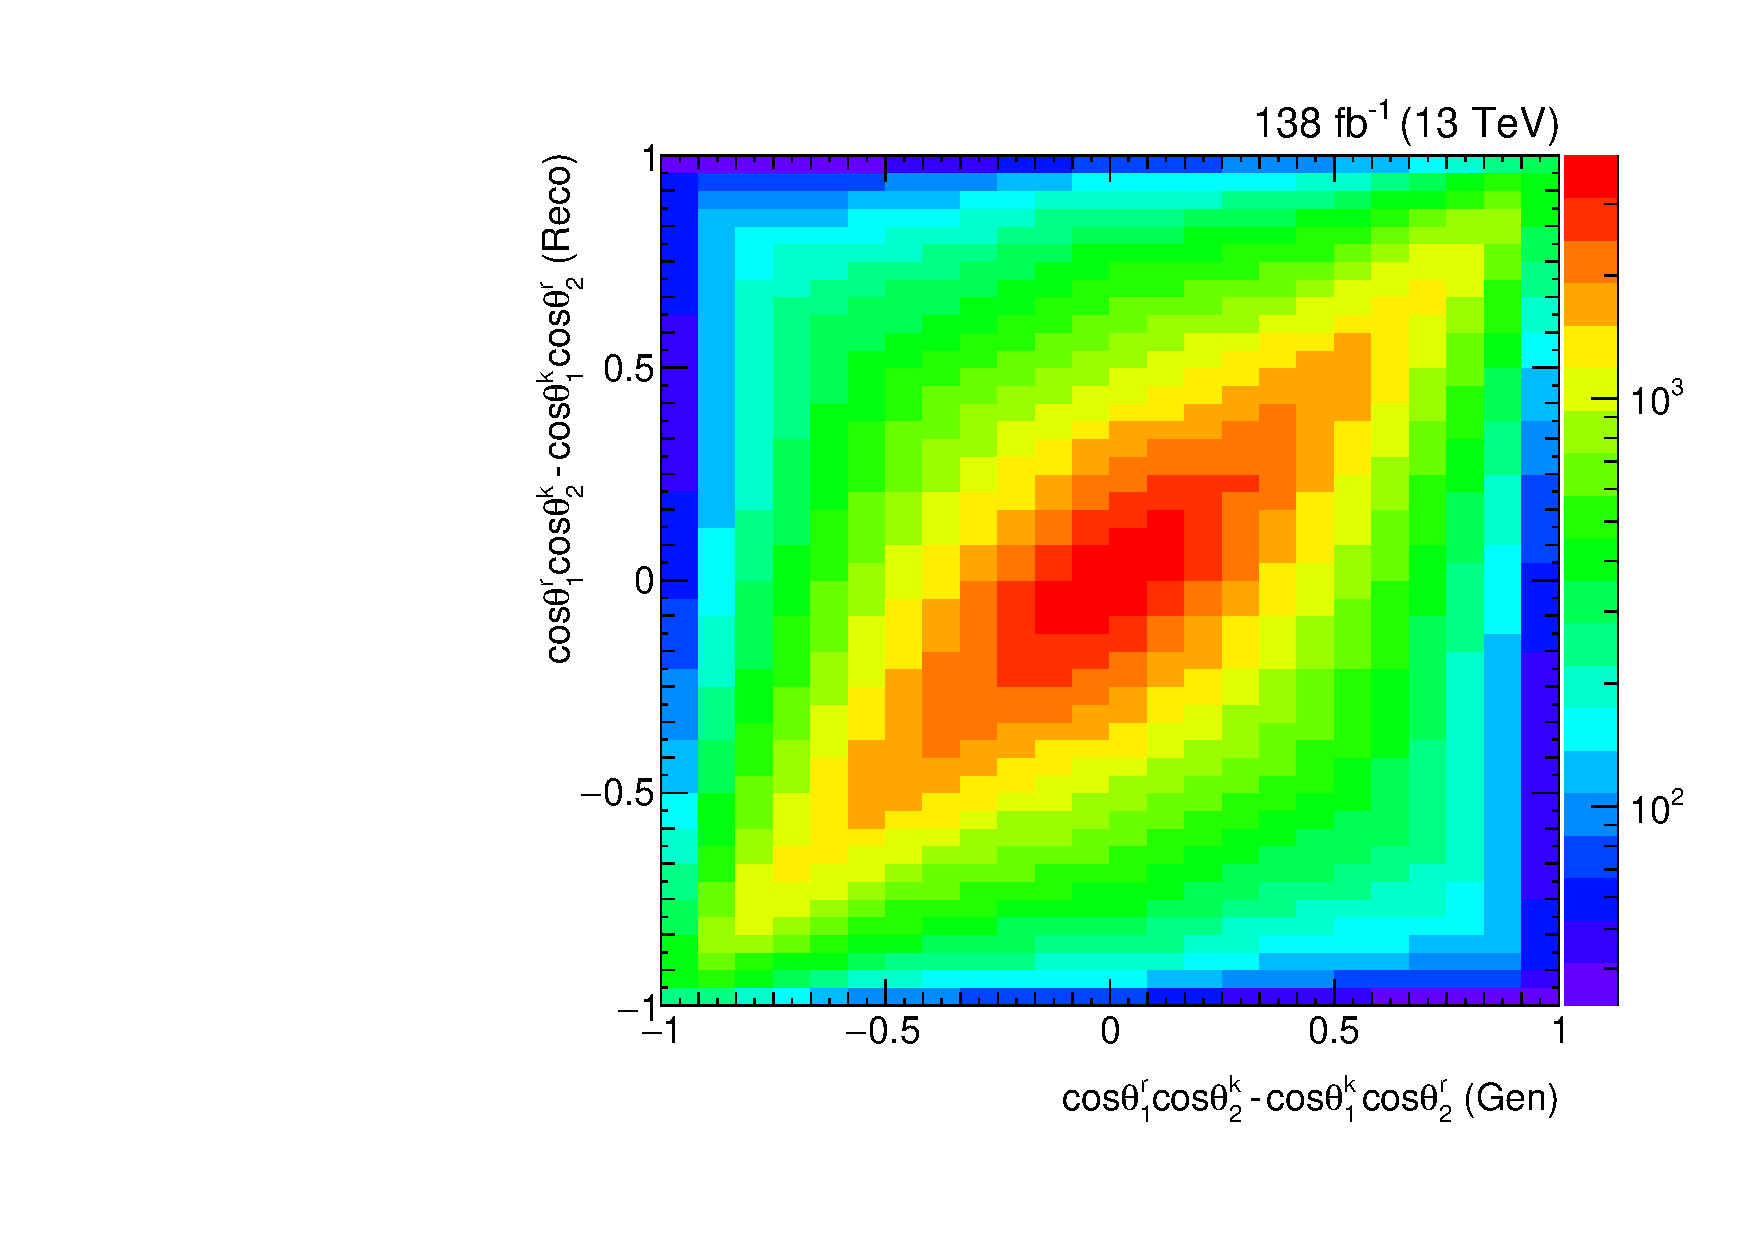
\includegraphics[width=0.40\textwidth]{fig_fullRun2UL/unfolding/combined/ResponseMatrix_c_Mrk.pdf} \\
 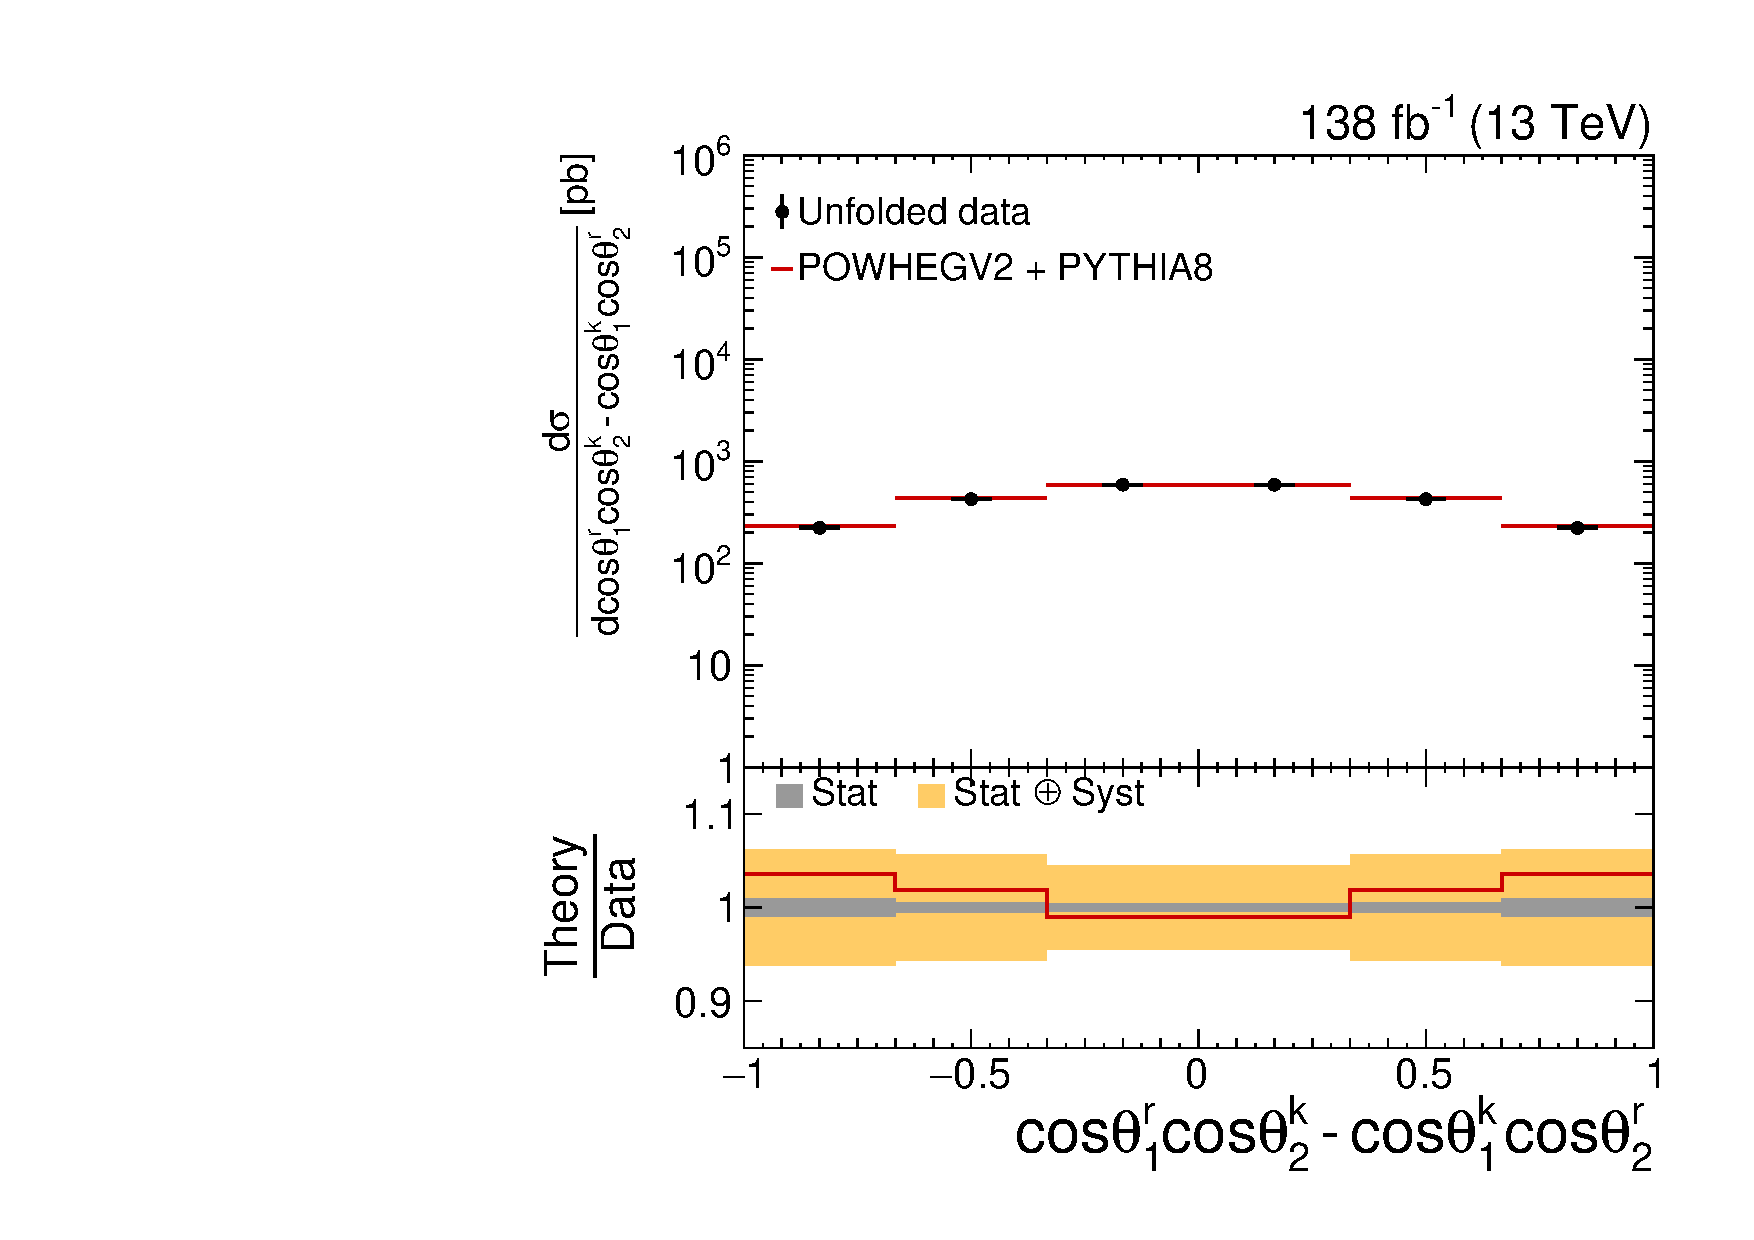
\includegraphics[width=0.40\textwidth]{fig_fullRun2UL/unfolding/combined/UnfoldedResults_c_Mrk.pdf}
 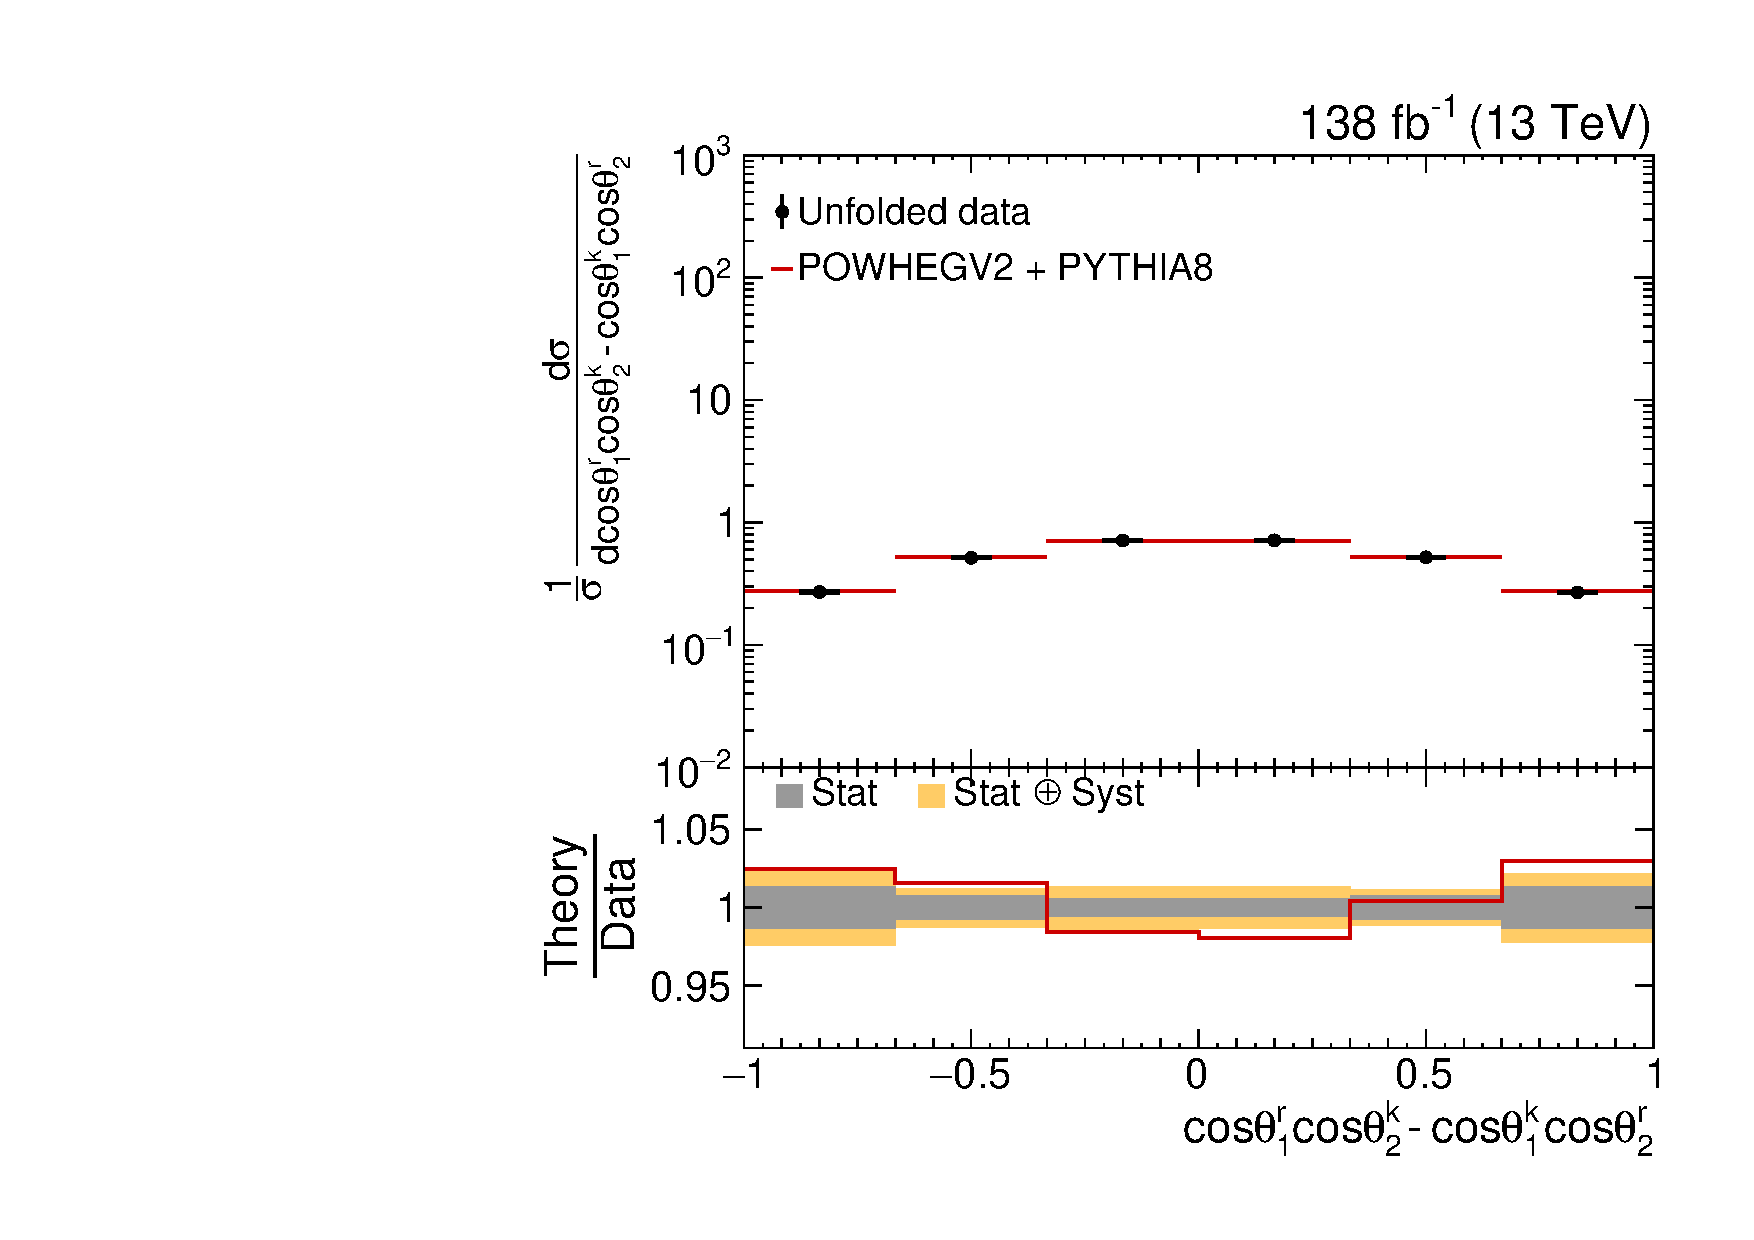
\includegraphics[width=0.40\textwidth]{fig_fullRun2UL/unfolding/combined/UnfoldedResultsNorm_c_Mrk.pdf} \\
\label{fig:c_Mrk}
\caption{Reconstructed detector-level distribution (Top Left), detector response-matrix (Top Right), absolute cross-section unfolded to parton-level (Bottom Left), and normalized cross-section unfolded to parton-level (Bottom Right) for off-diagonal spin correlation difference observable $\cos\theta_{1}^{r}\cos\theta_{2}^{k}-\cos\theta_{1}^{k}\cos\theta_{2}^{r}$, from which spin-density coefficient $C_{rk}-C_{kr}$ (sensitive to spin-density coefficient function $c_n$) is extracted.}
\end{center}
\end{figure}
\clearpage
\begin{figure}[htb]
\begin{center}
 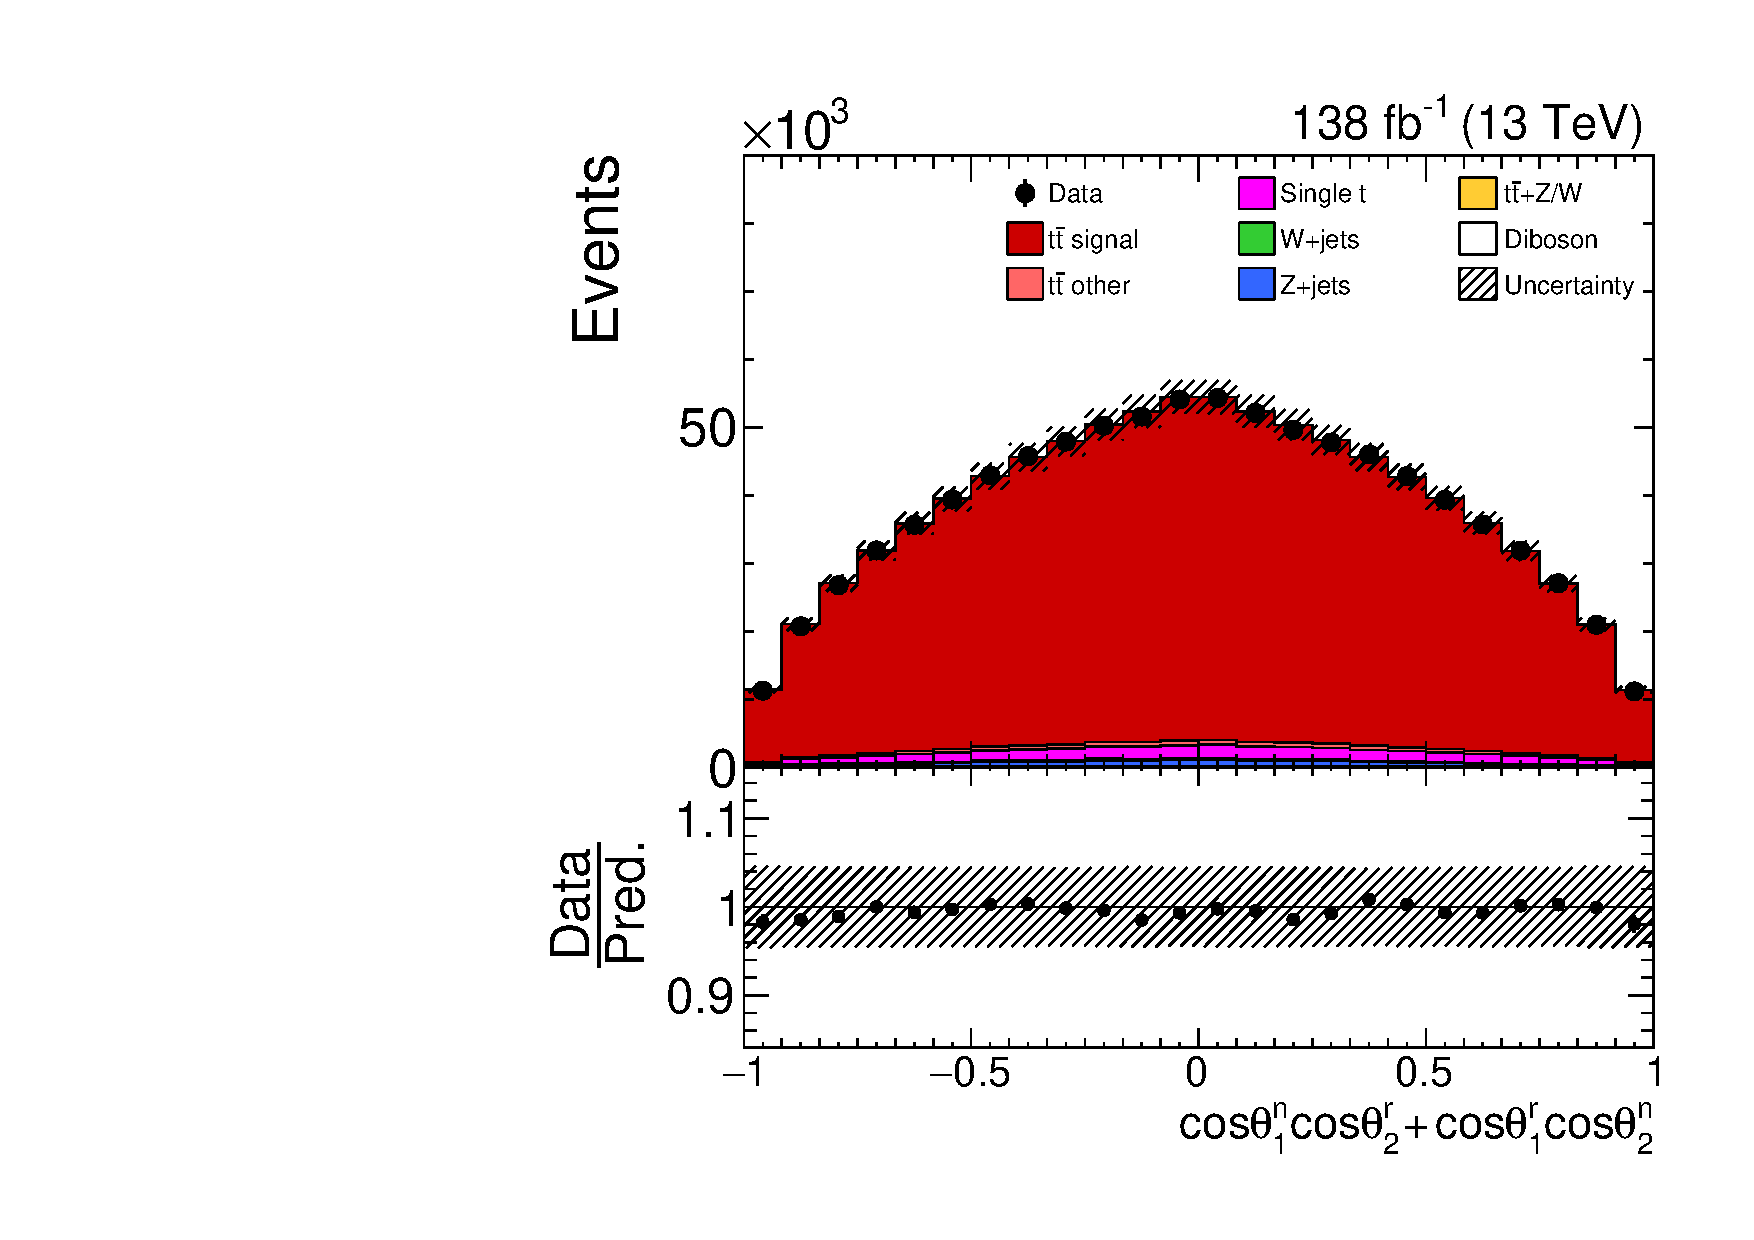
\includegraphics[width=0.40\textwidth]{fig_fullRun2UL/controlplots/combined/Hyp_LLBarCPnr.pdf}
 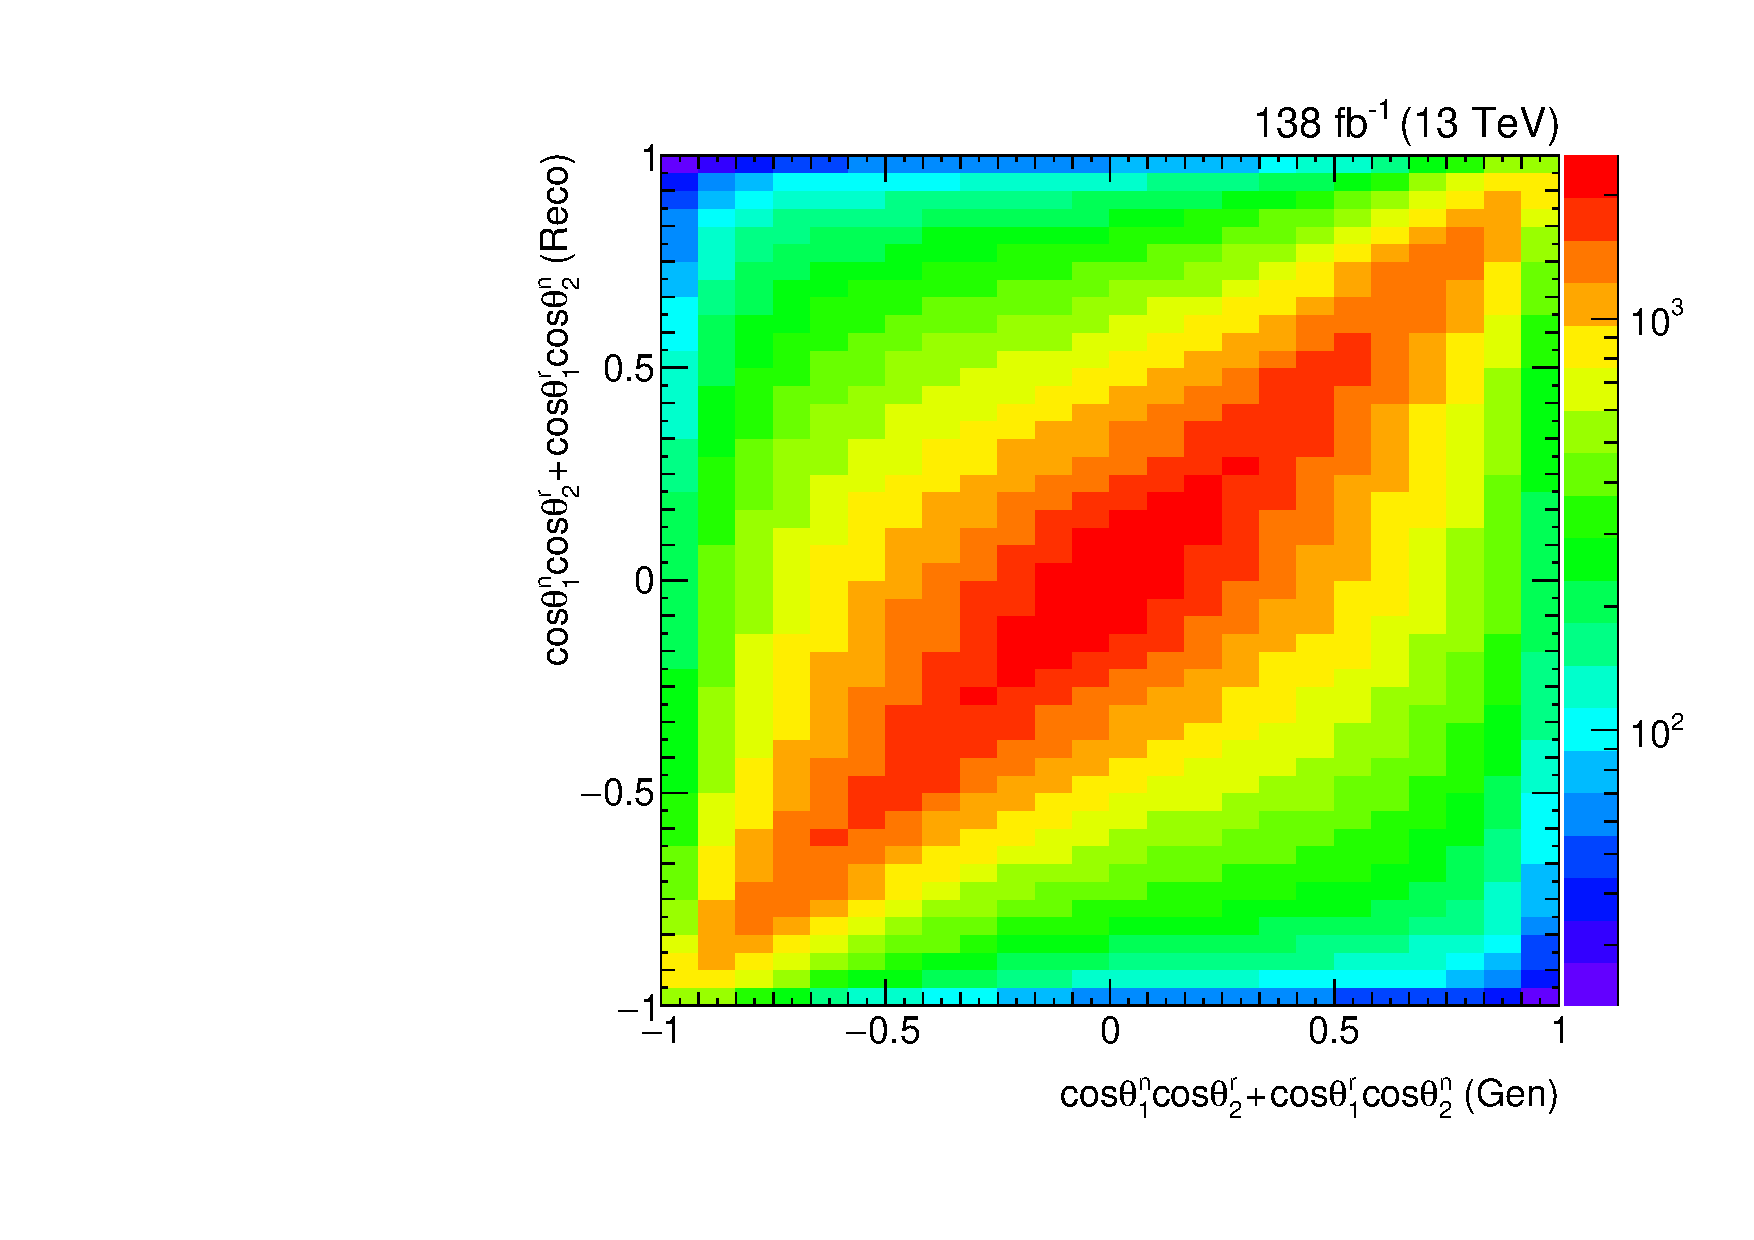
\includegraphics[width=0.40\textwidth]{fig_fullRun2UL/unfolding/combined/ResponseMatrix_c_Pnr.pdf} \\
 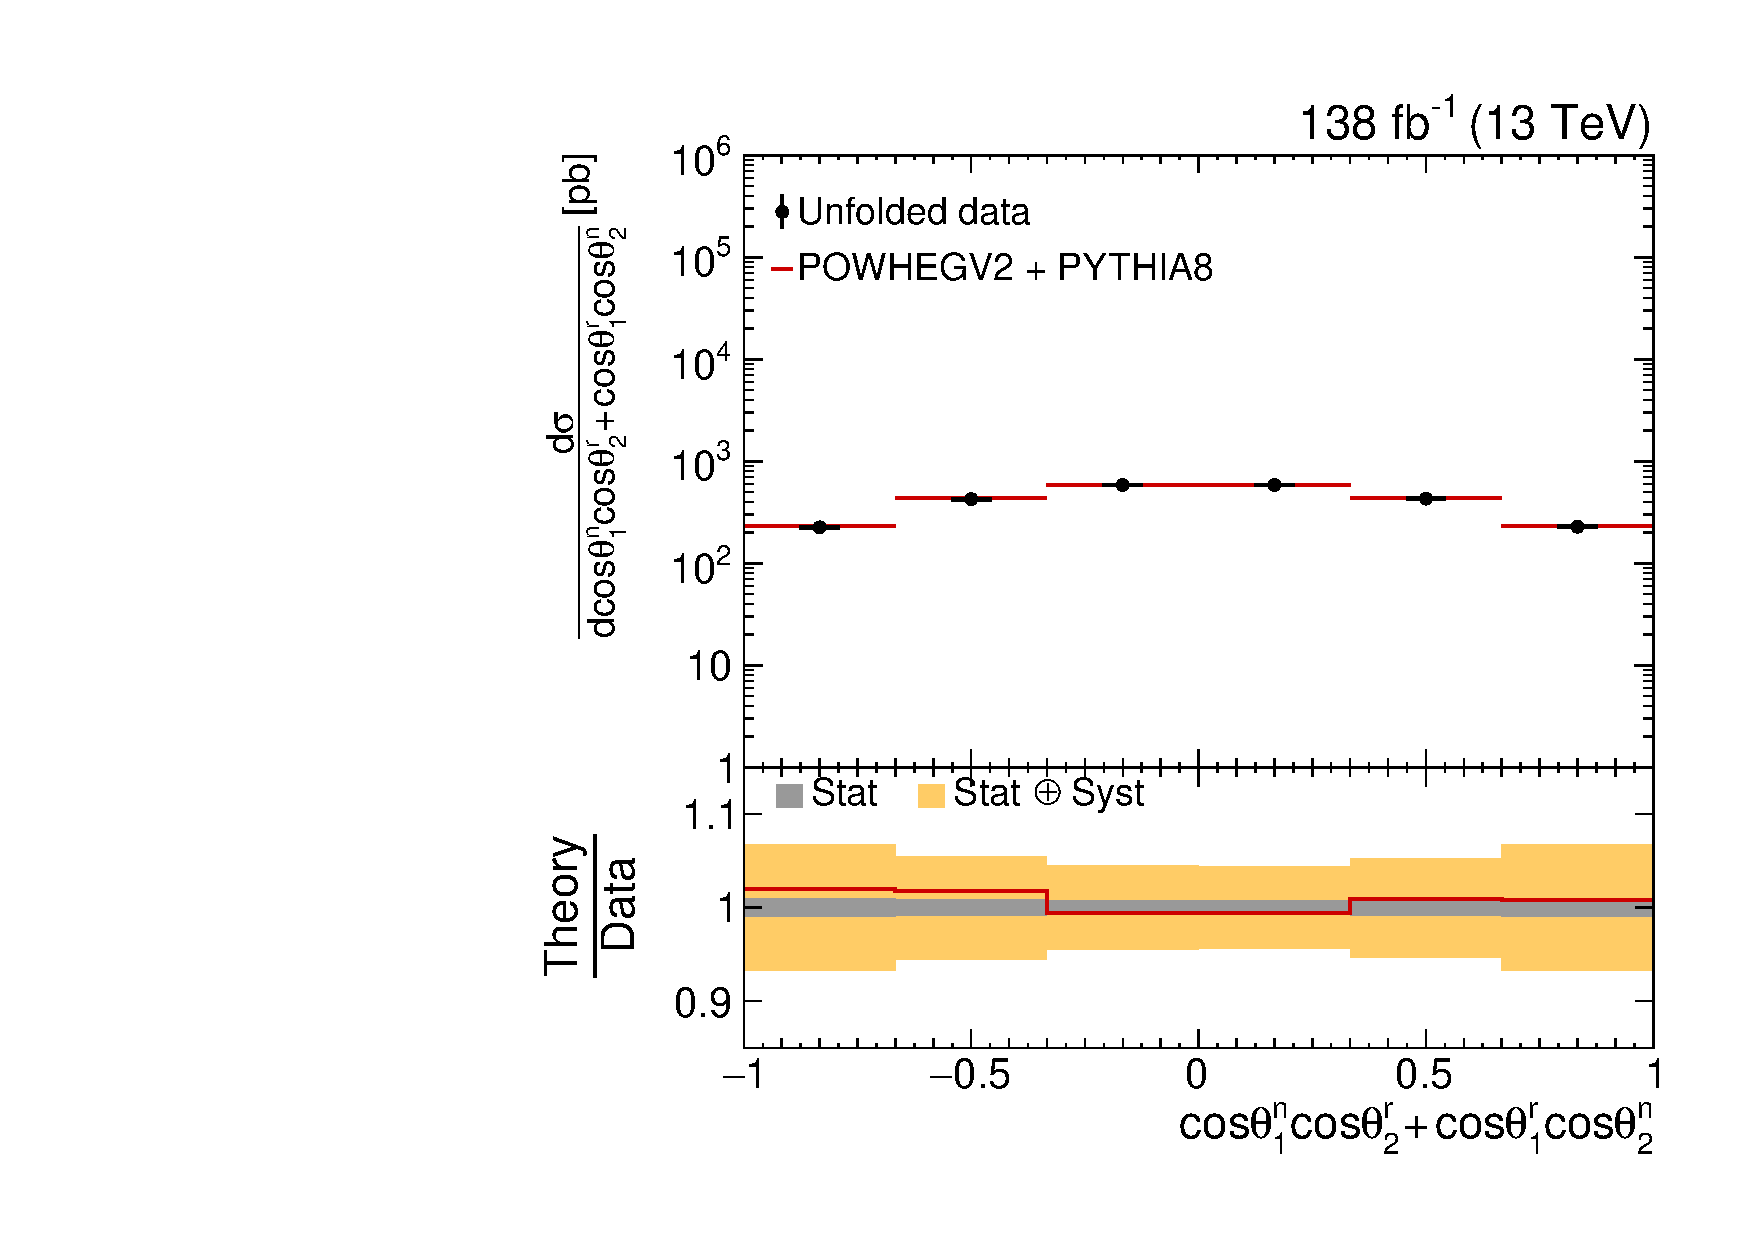
\includegraphics[width=0.40\textwidth]{fig_fullRun2UL/unfolding/combined/UnfoldedResults_c_Pnr.pdf}
 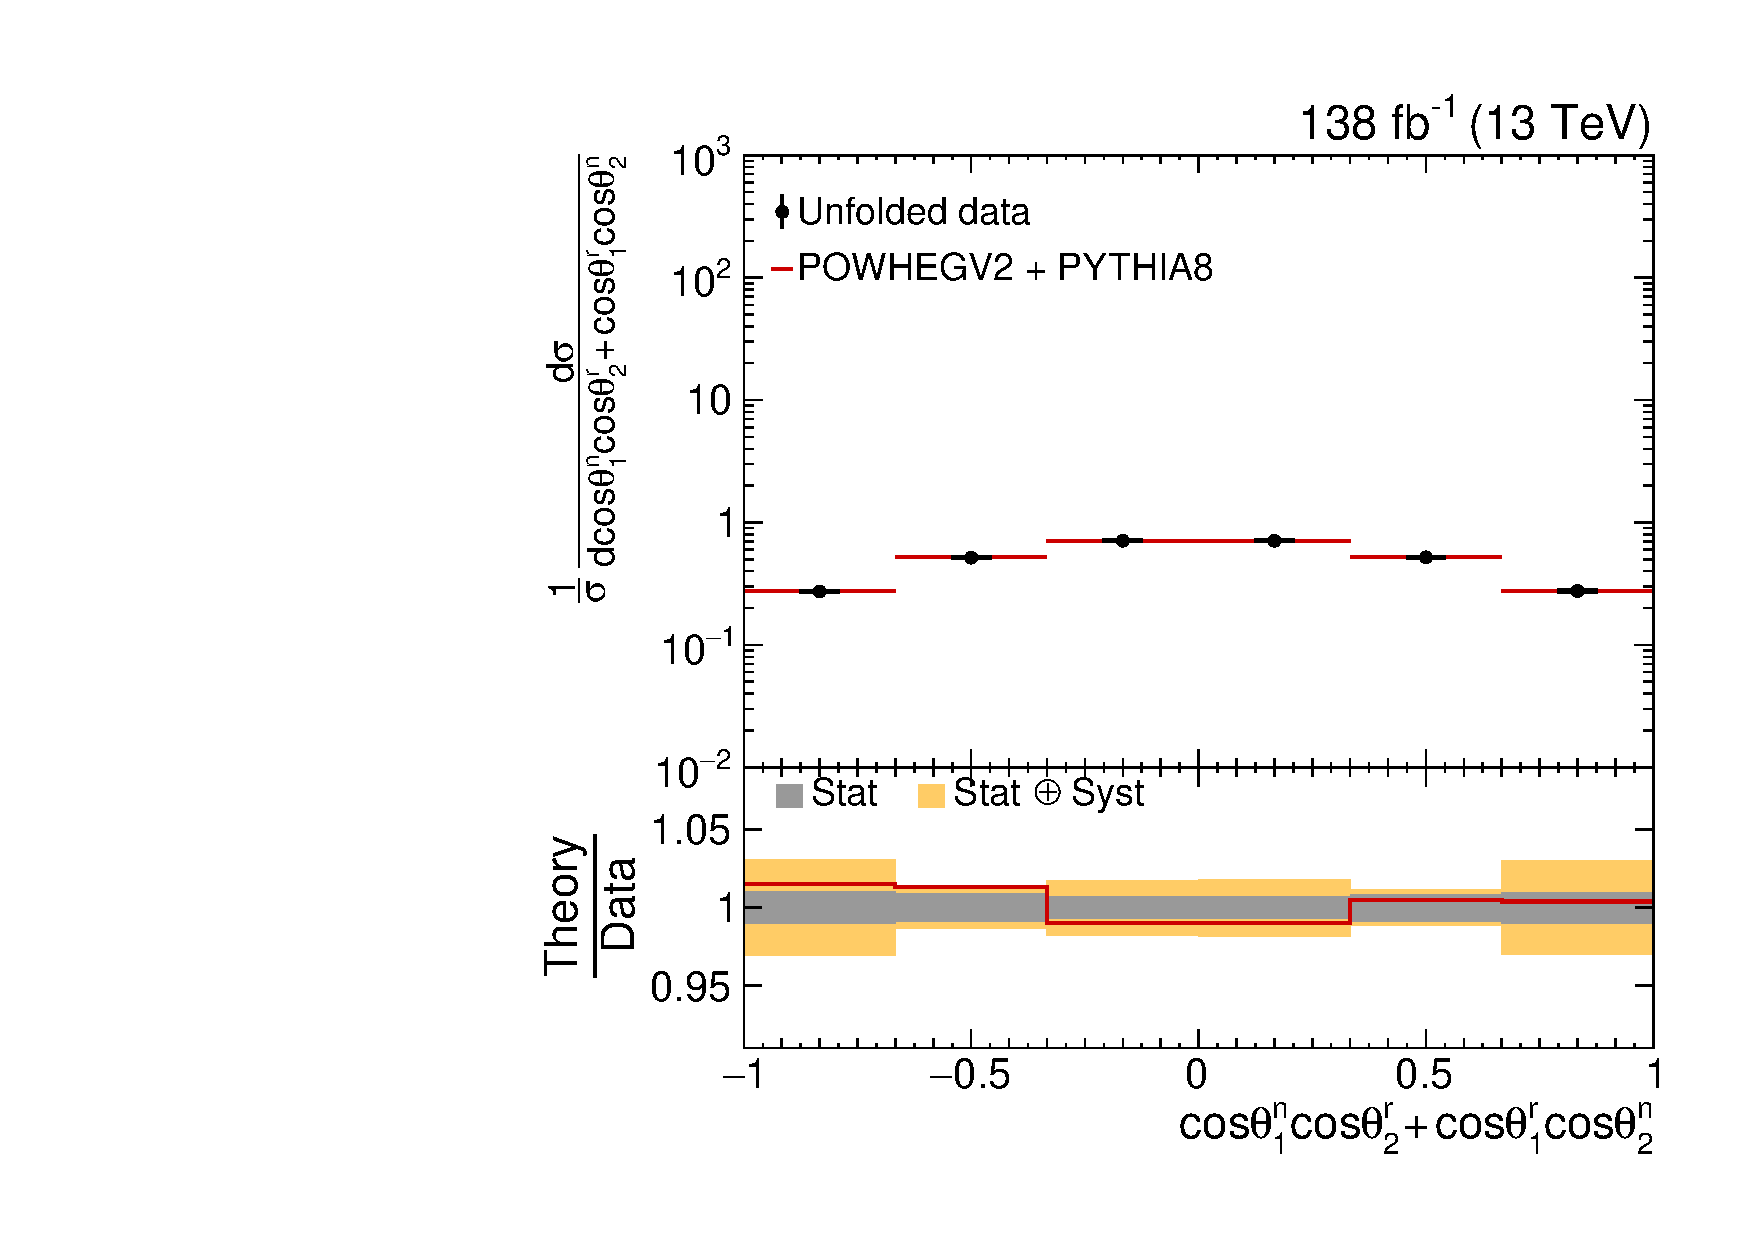
\includegraphics[width=0.40\textwidth]{fig_fullRun2UL/unfolding/combined/UnfoldedResultsNorm_c_Pnr.pdf} \\
\label{fig:c_Pnr}
\caption{Reconstructed detector-level distribution (Top Left), detector response-matrix (Top Right), absolute cross-section unfolded to parton-level (Bottom Left), and normalized cross-section unfolded to parton-level (Bottom Right) for off-diagonal spin correlation sum observable $\cos\theta_{1}^{n}\cos\theta_{2}^{r}+\cos\theta_{1}^{r}\cos\theta_{2}^{n}$, from which spin-density coefficient $C_{nr}+C_{rn}$ (sensitive to spin-density coefficient function $c_{n r}$) is extracted.}
\end{center}
\end{figure}
\clearpage
\begin{figure}[htb]
\begin{center}
 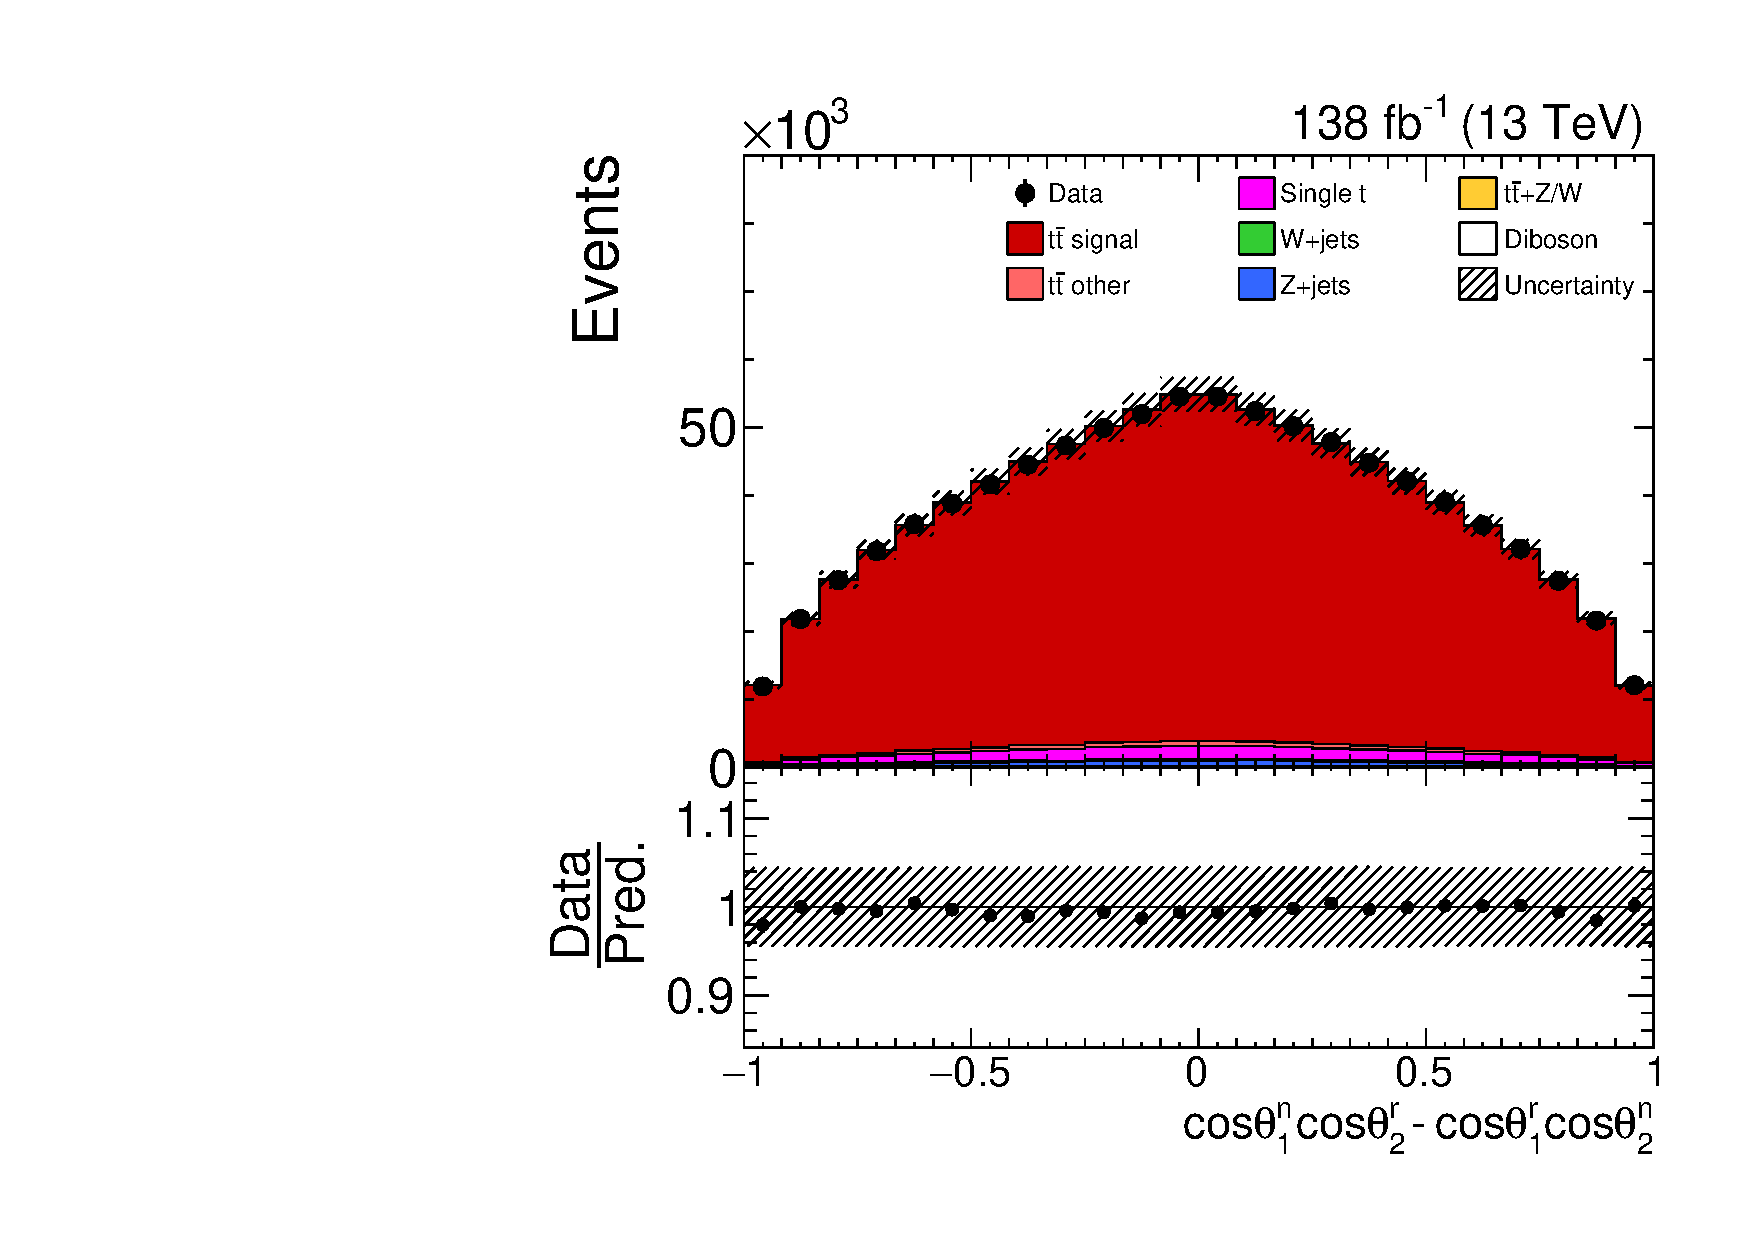
\includegraphics[width=0.40\textwidth]{fig_fullRun2UL/controlplots/combined/Hyp_LLBarCMnr.pdf}
 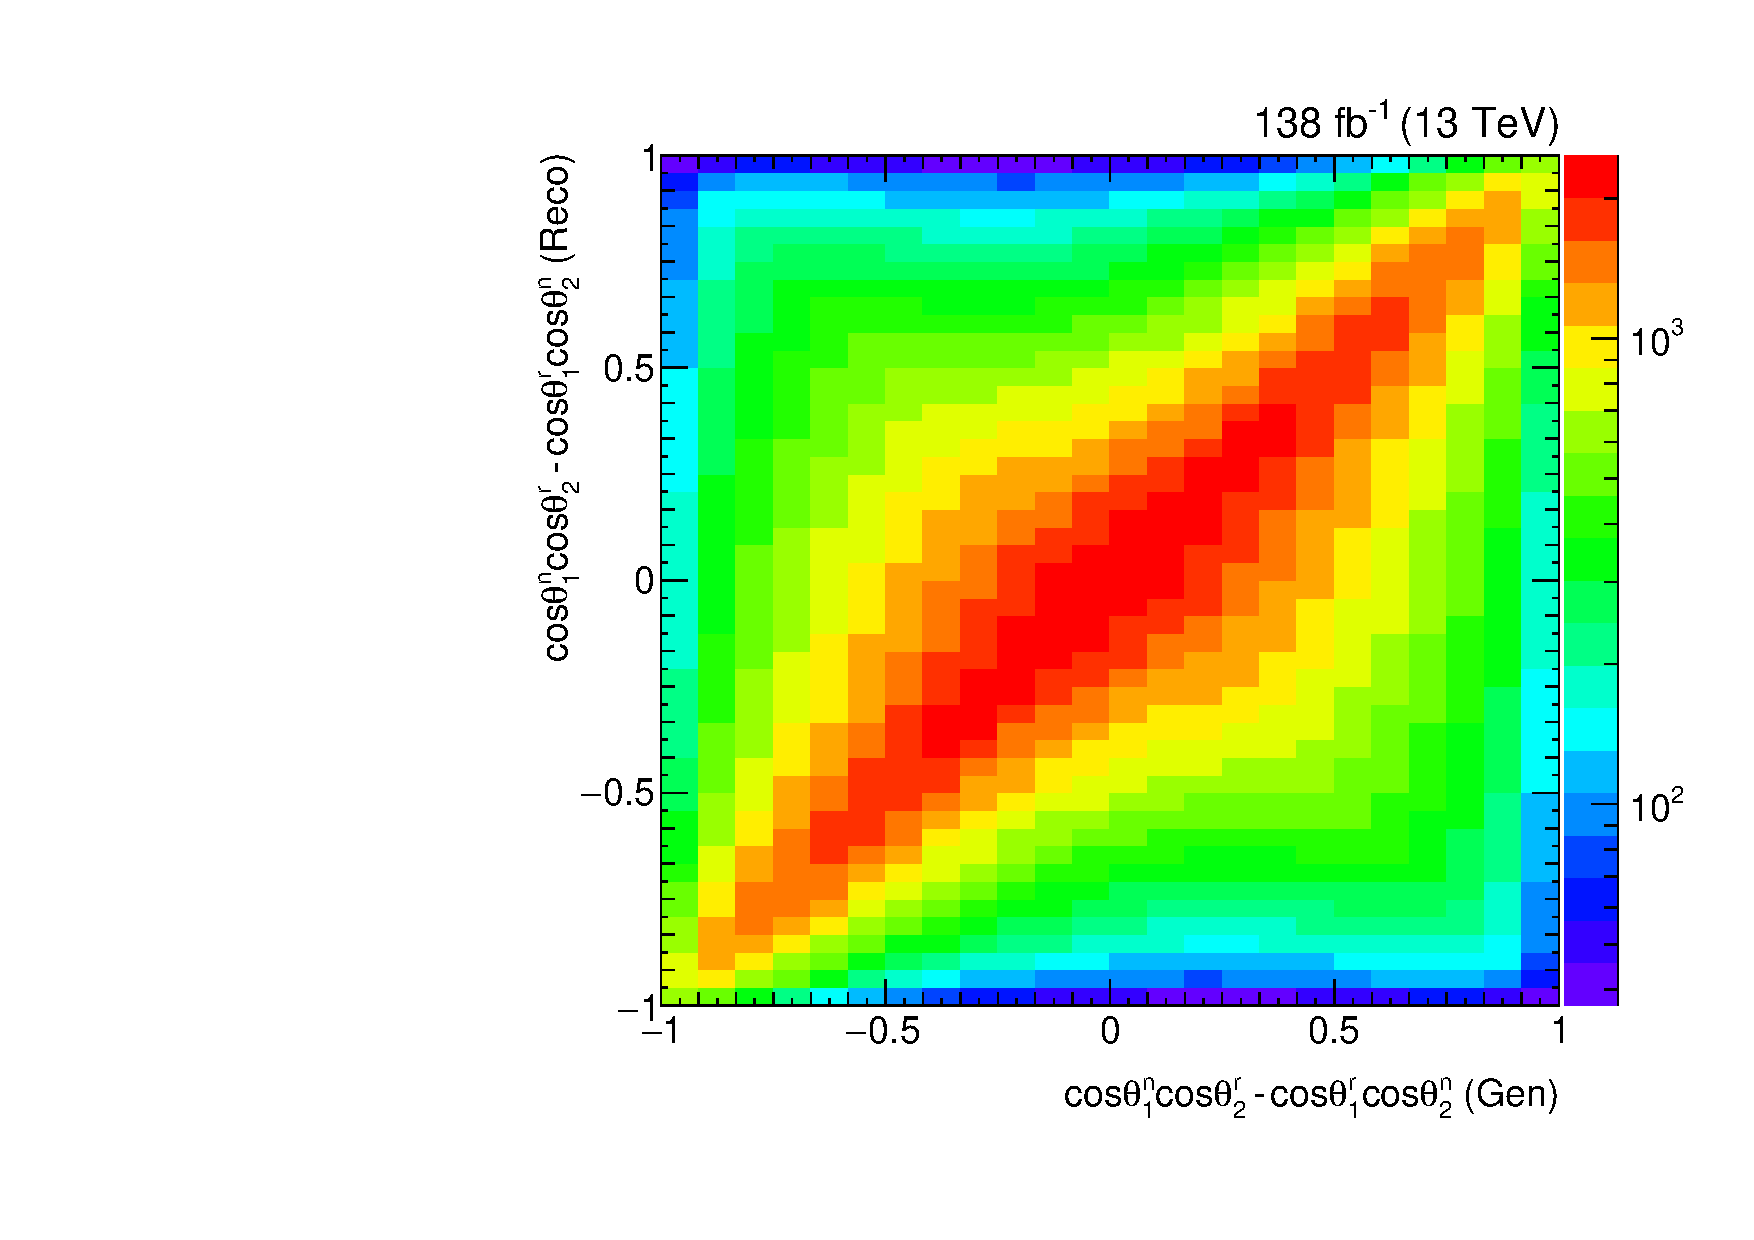
\includegraphics[width=0.40\textwidth]{fig_fullRun2UL/unfolding/combined/ResponseMatrix_c_Mnr.pdf} \\
 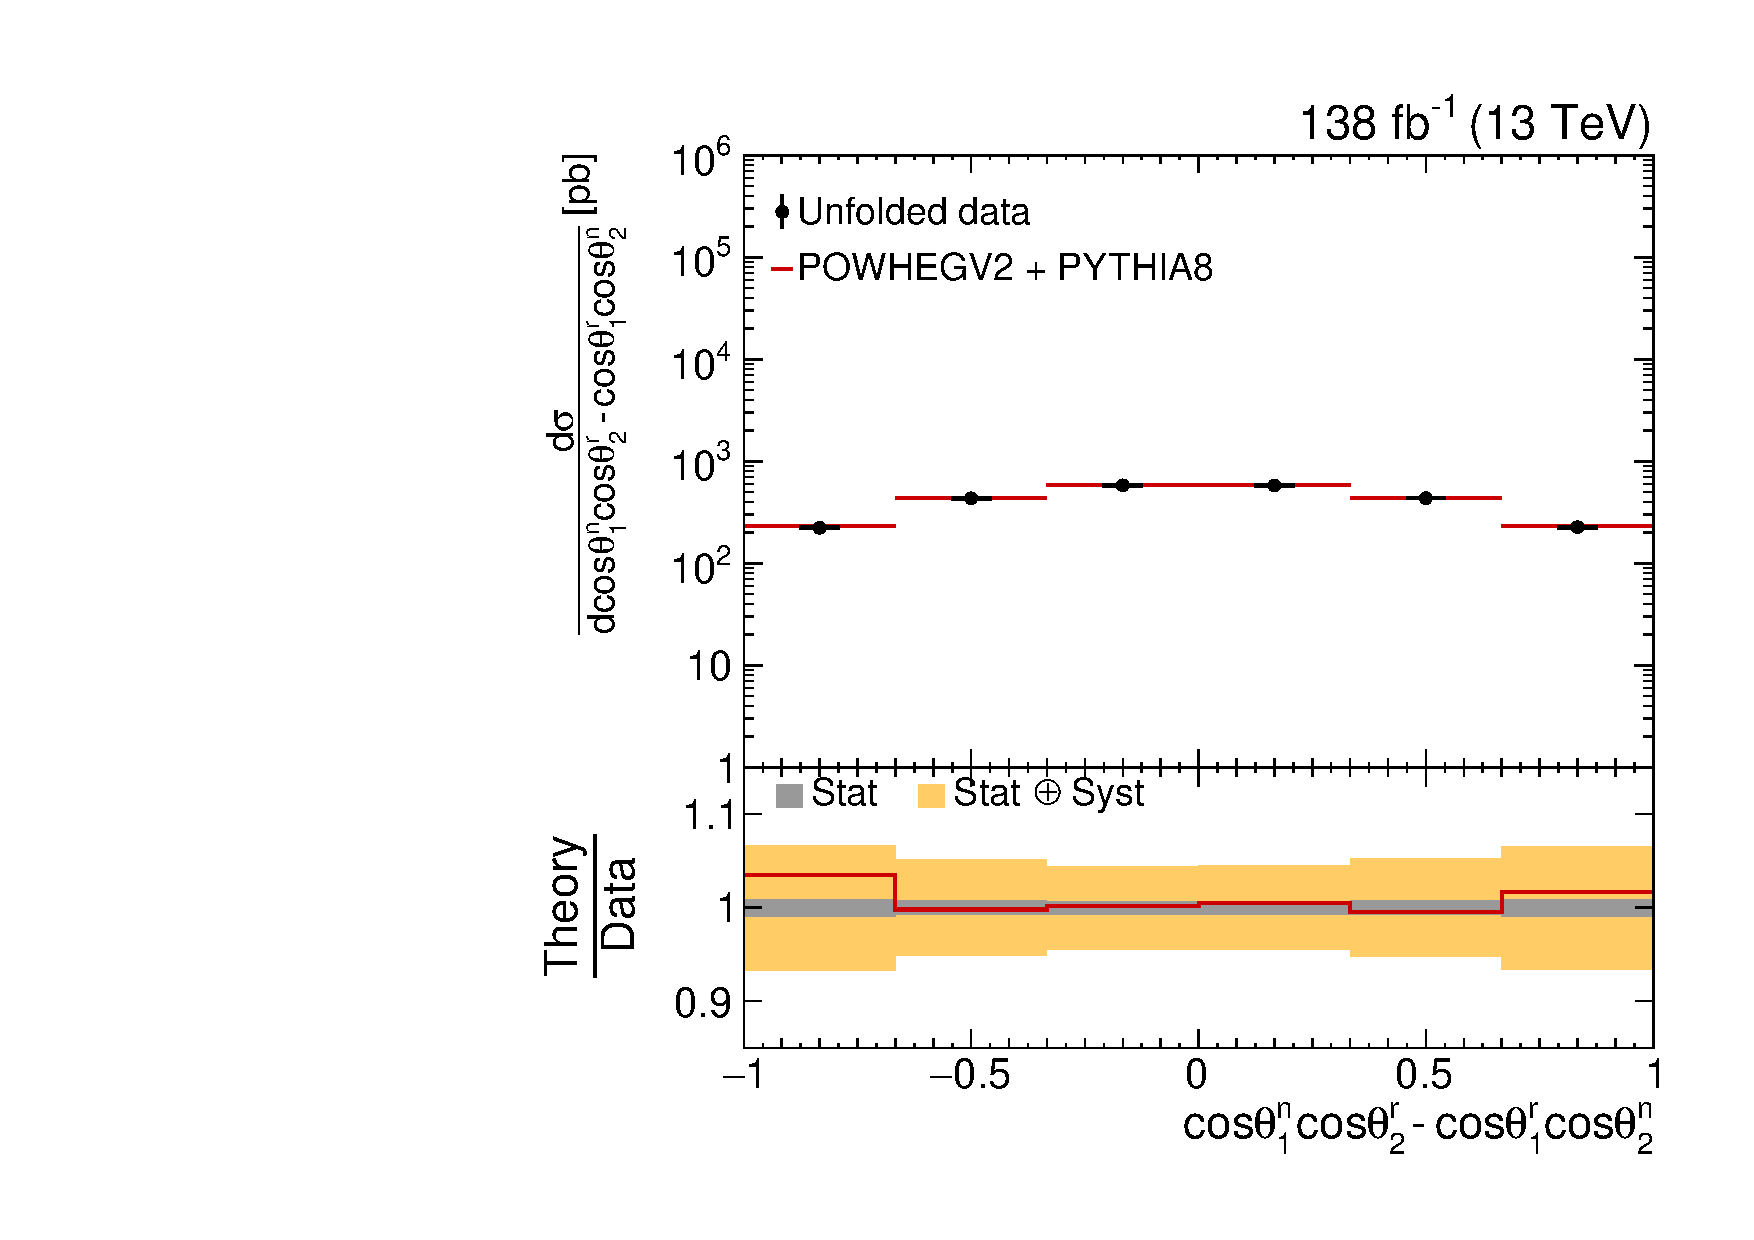
\includegraphics[width=0.40\textwidth]{fig_fullRun2UL/unfolding/combined/UnfoldedResults_c_Mnr.pdf}
 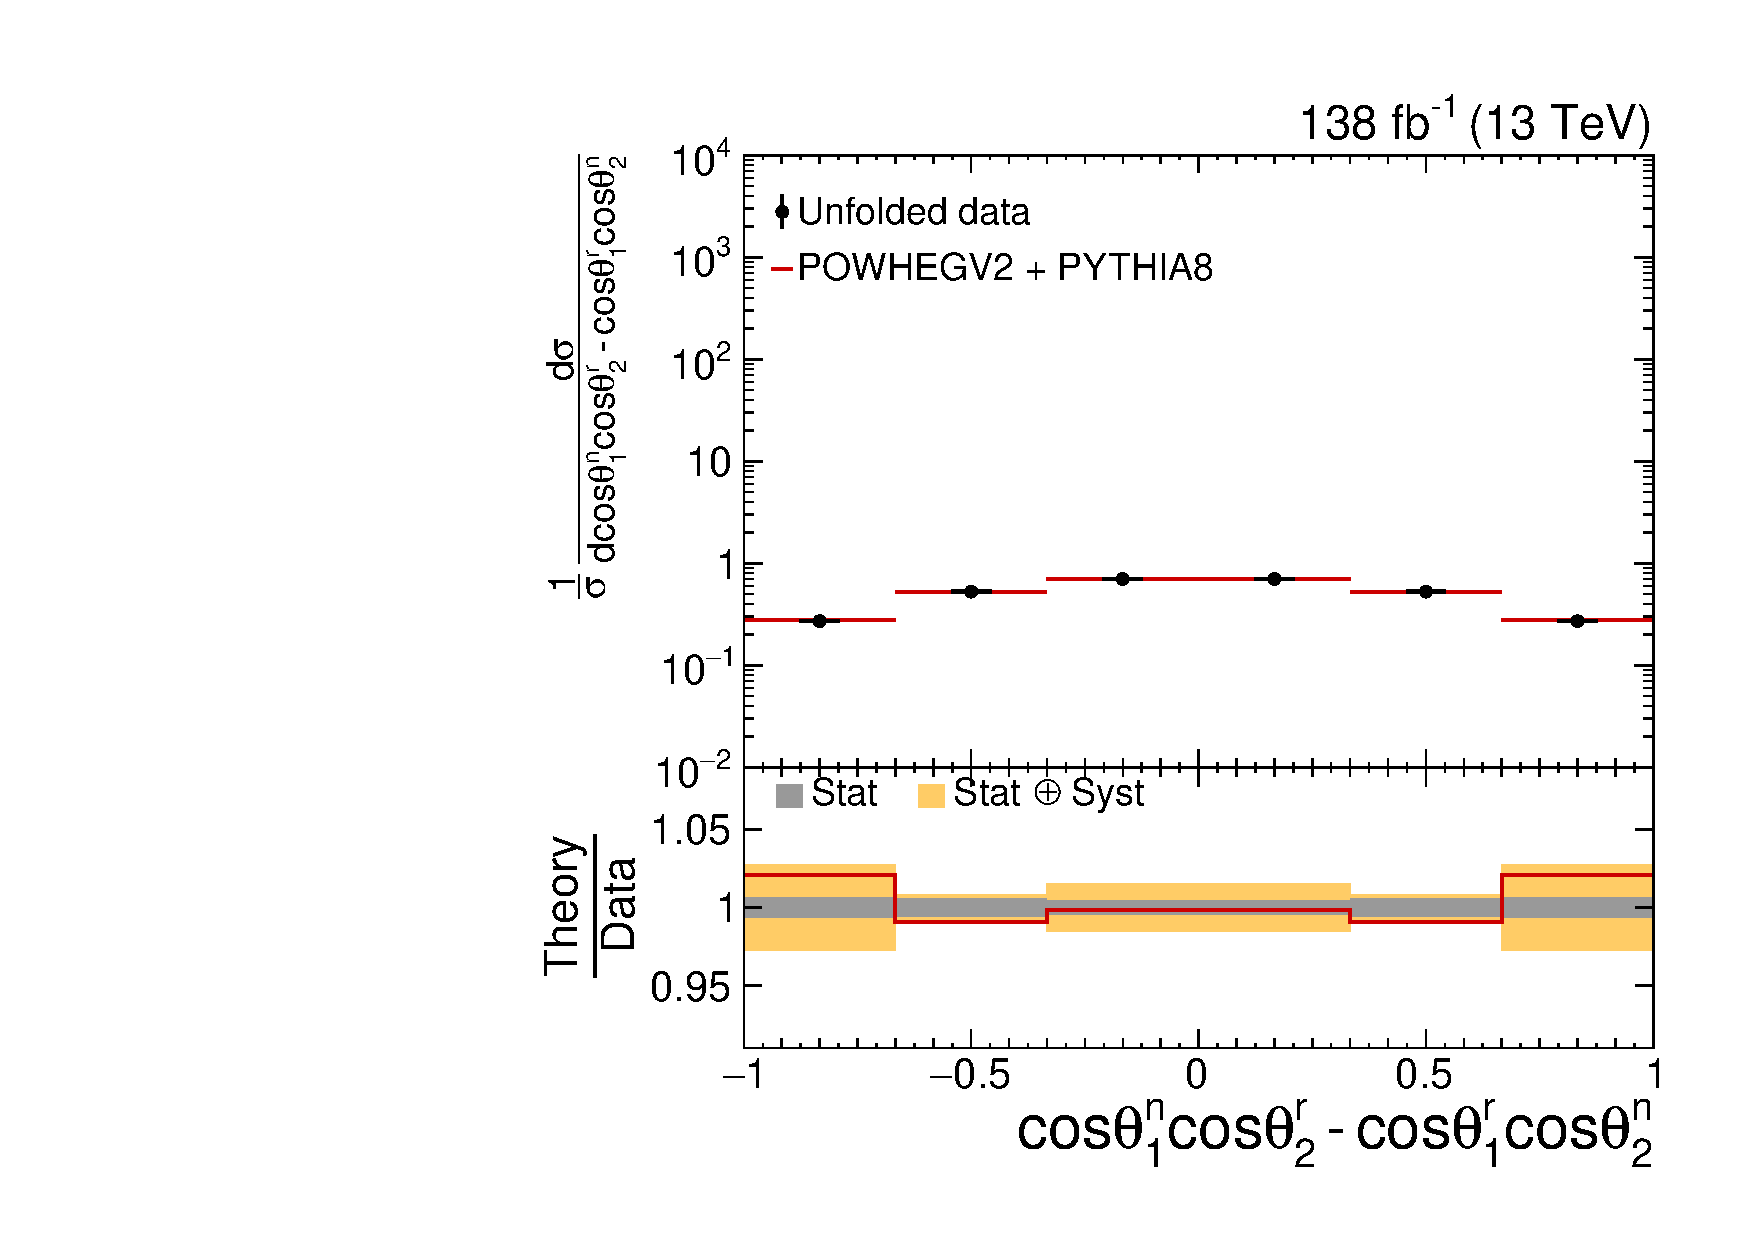
\includegraphics[width=0.40\textwidth]{fig_fullRun2UL/unfolding/combined/UnfoldedResultsNorm_c_Mnr.pdf} \\
\label{fig:c_Mnr}
\caption{Reconstructed detector-level distribution (Top Left), detector response-matrix (Top Right), absolute cross-section unfolded to parton-level (Bottom Left), and normalized cross-section unfolded to parton-level (Bottom Right) for off-diagonal spin correlation difference observable $\cos\theta_{1}^{n}\cos\theta_{2}^{r}-\cos\theta_{1}^{r}\cos\theta_{2}^{n}$, from which spin-density coefficient $C_{nr}-C_{rn}$ (sensitive to spin-density coefficient function $c_k$) is extracted.}
\end{center}
\end{figure}
\clearpage
\begin{figure}[htb]
\begin{center}
 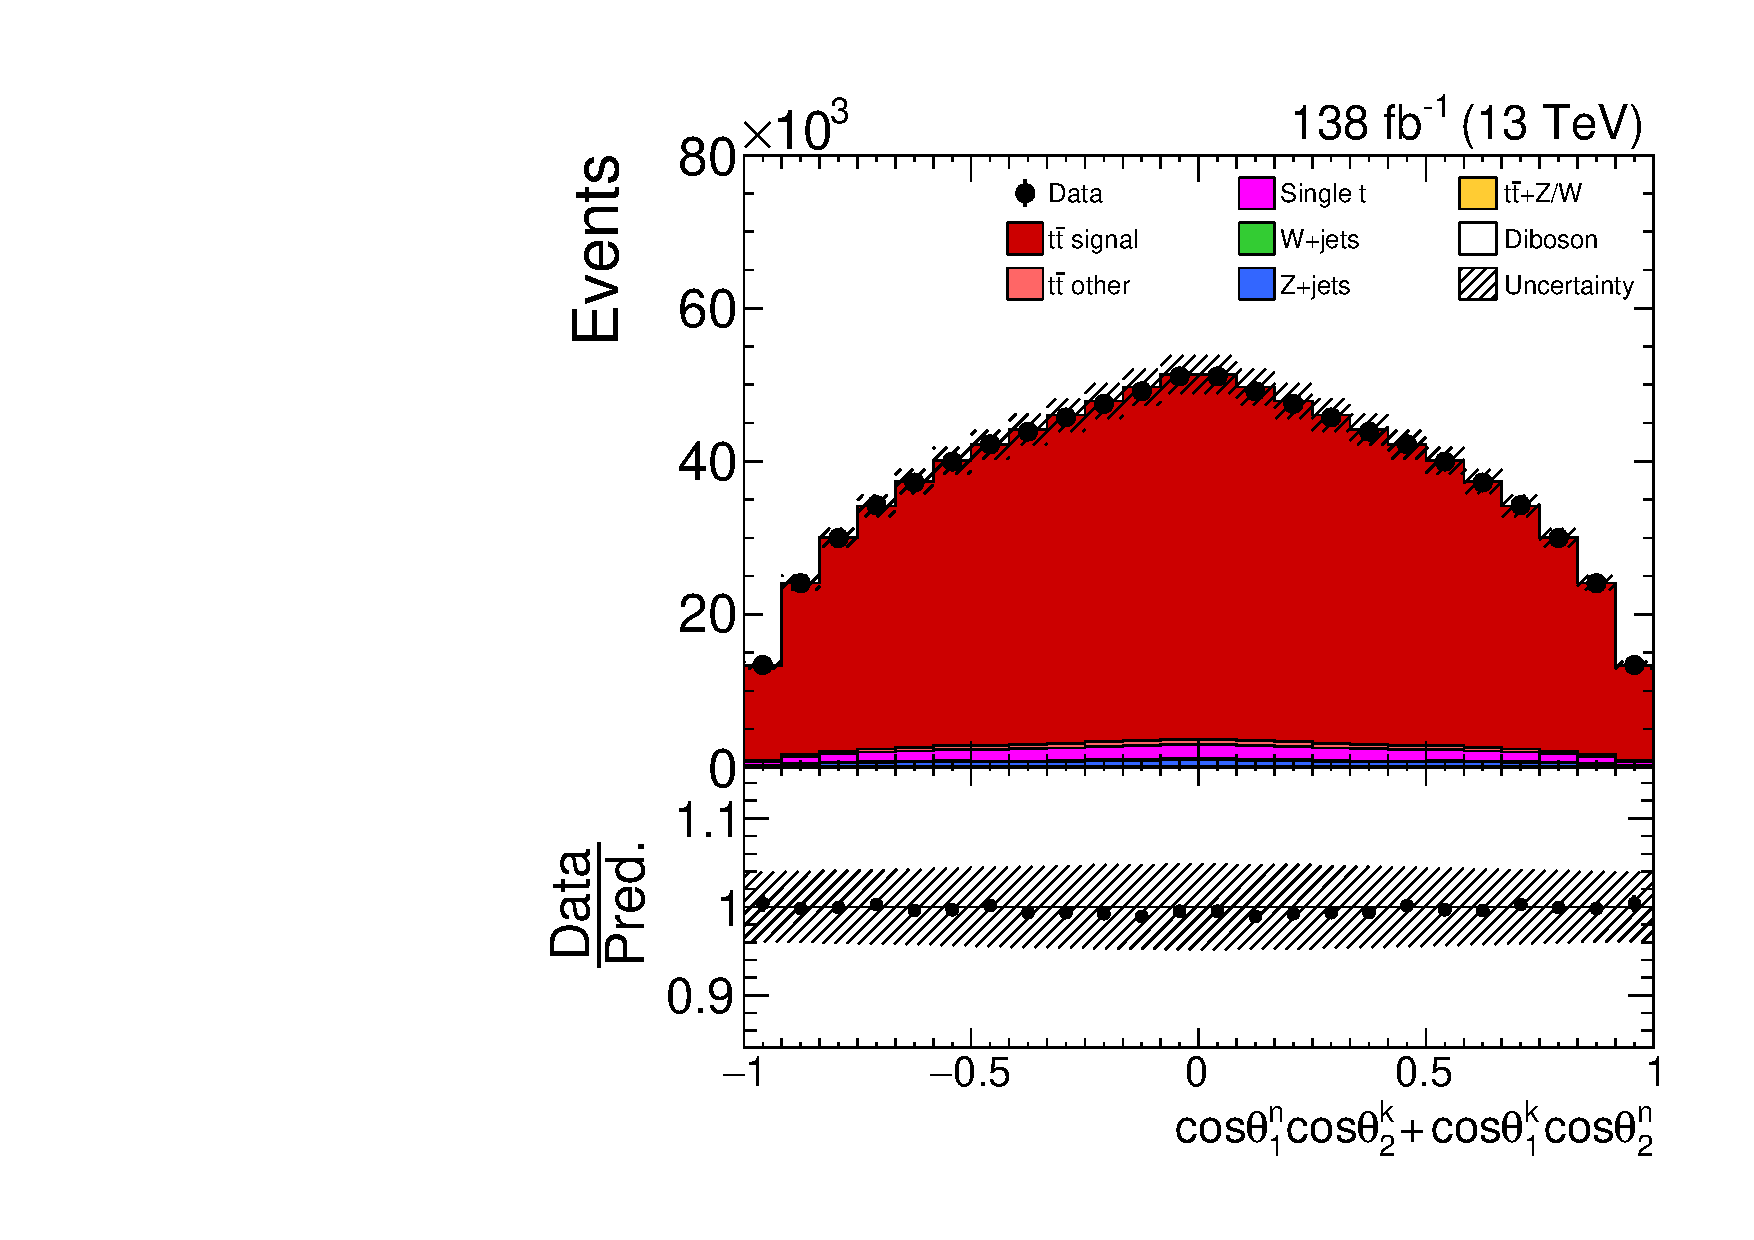
\includegraphics[width=0.40\textwidth]{fig_fullRun2UL/controlplots/combined/Hyp_LLBarCPnk.pdf}
 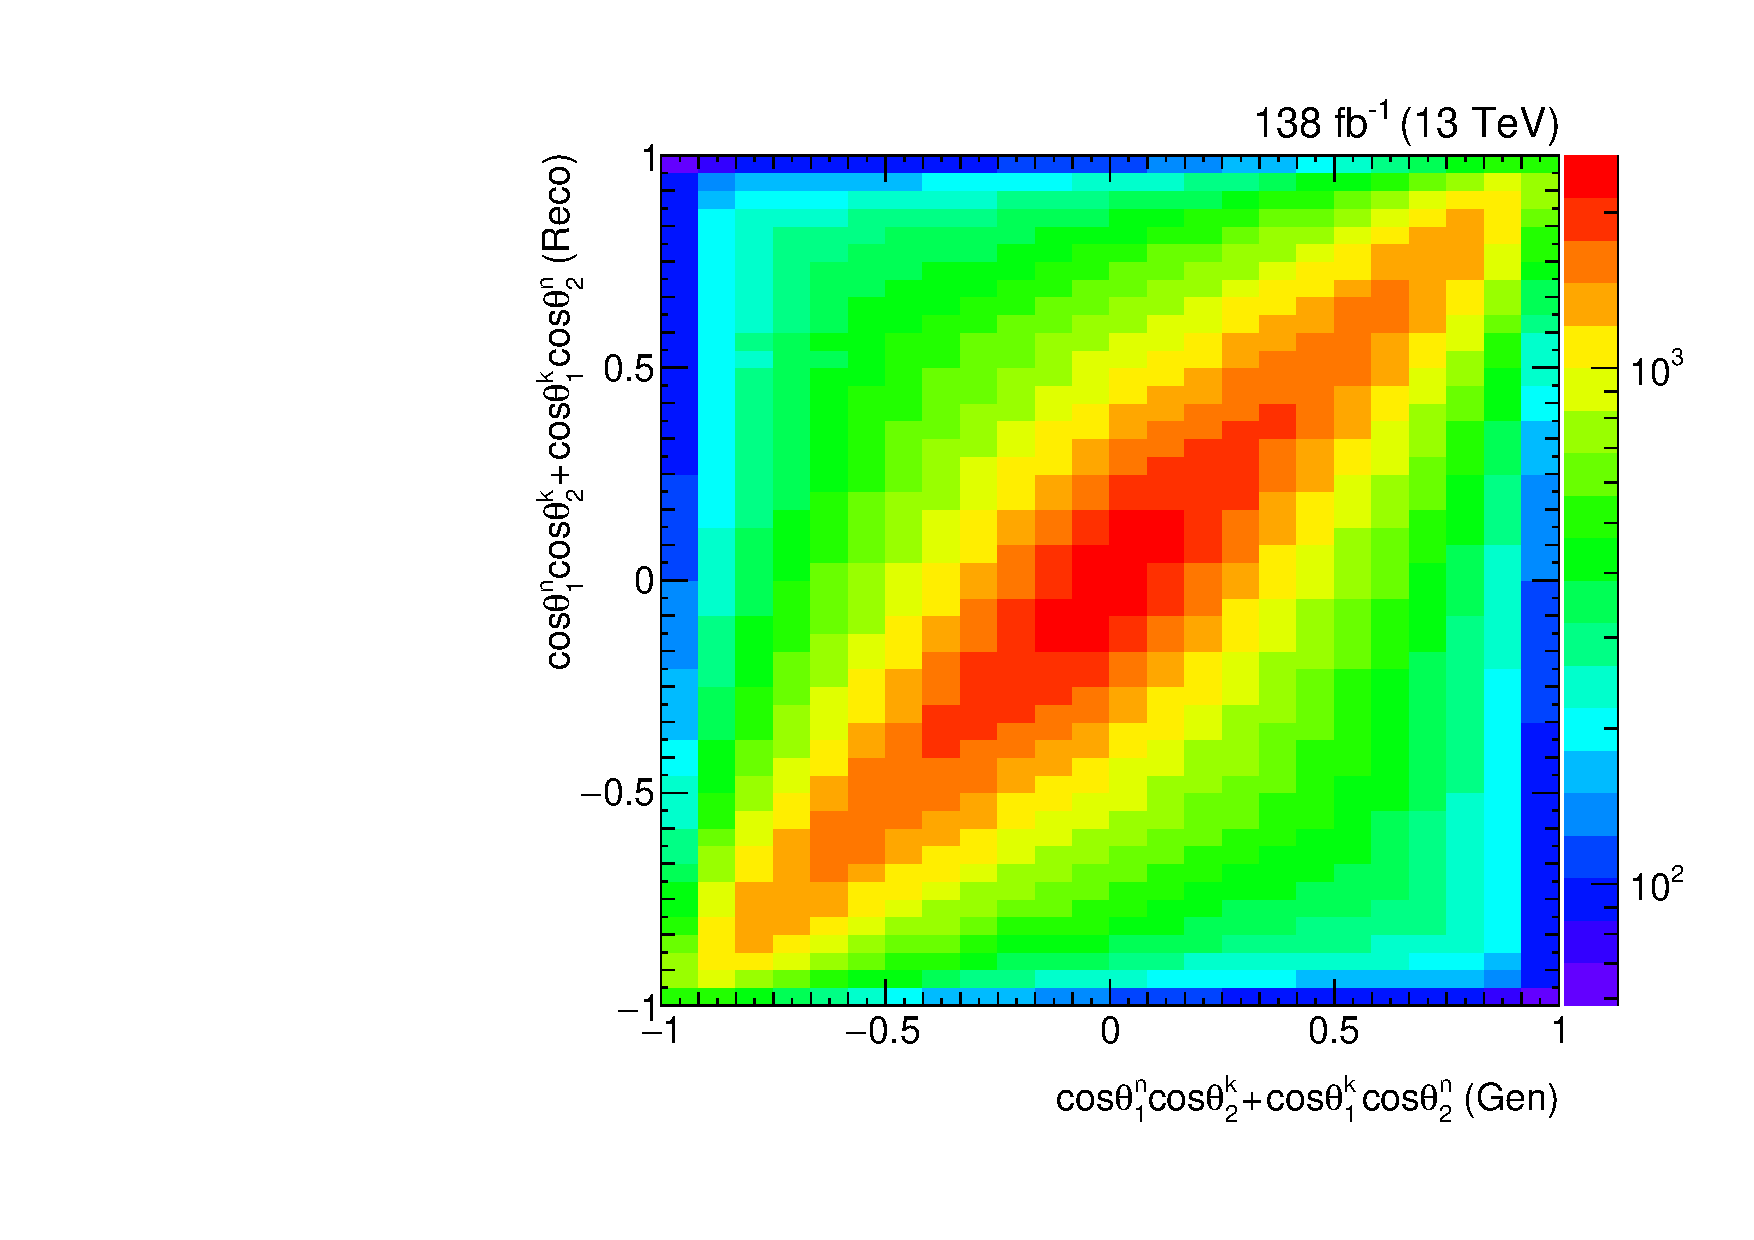
\includegraphics[width=0.40\textwidth]{fig_fullRun2UL/unfolding/combined/ResponseMatrix_c_Pnk.pdf} \\
 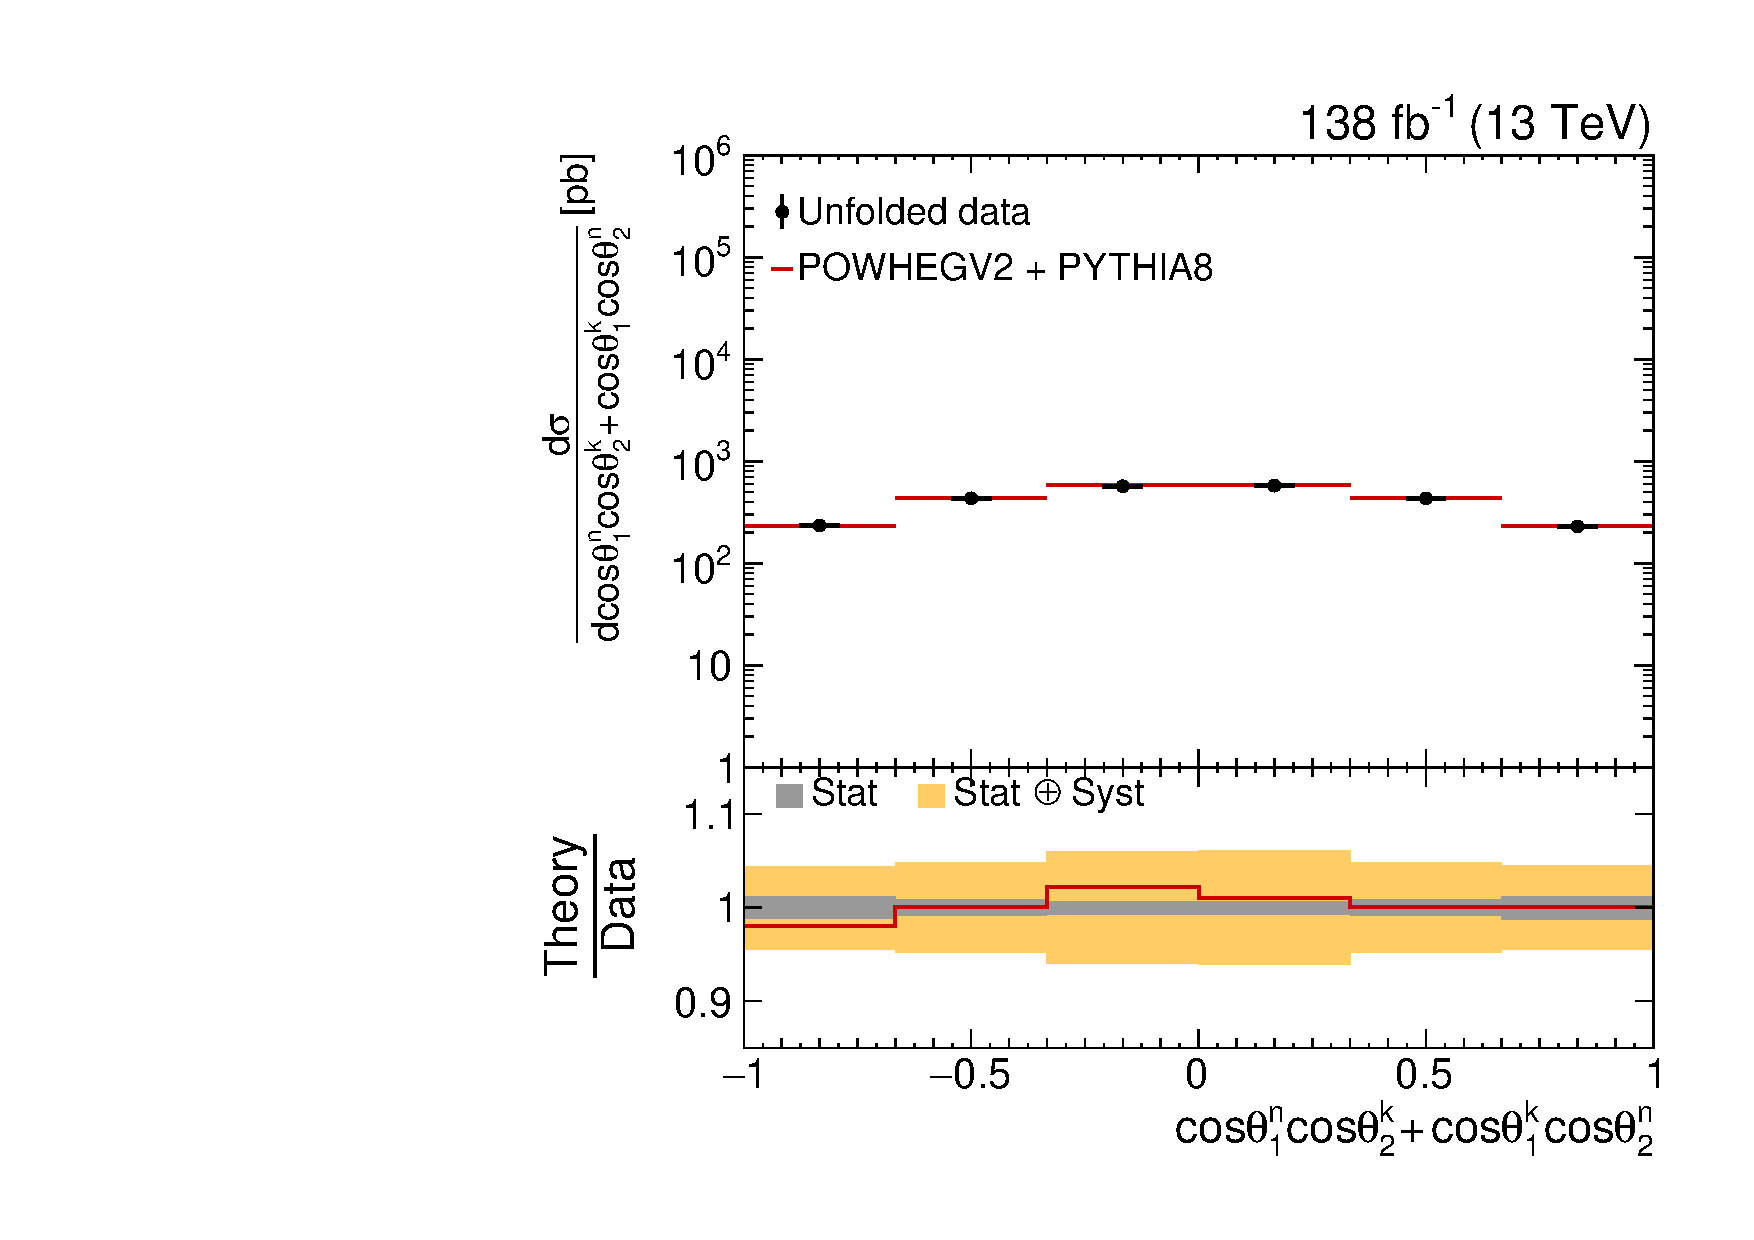
\includegraphics[width=0.40\textwidth]{fig_fullRun2UL/unfolding/combined/UnfoldedResults_c_Pnk.pdf}
 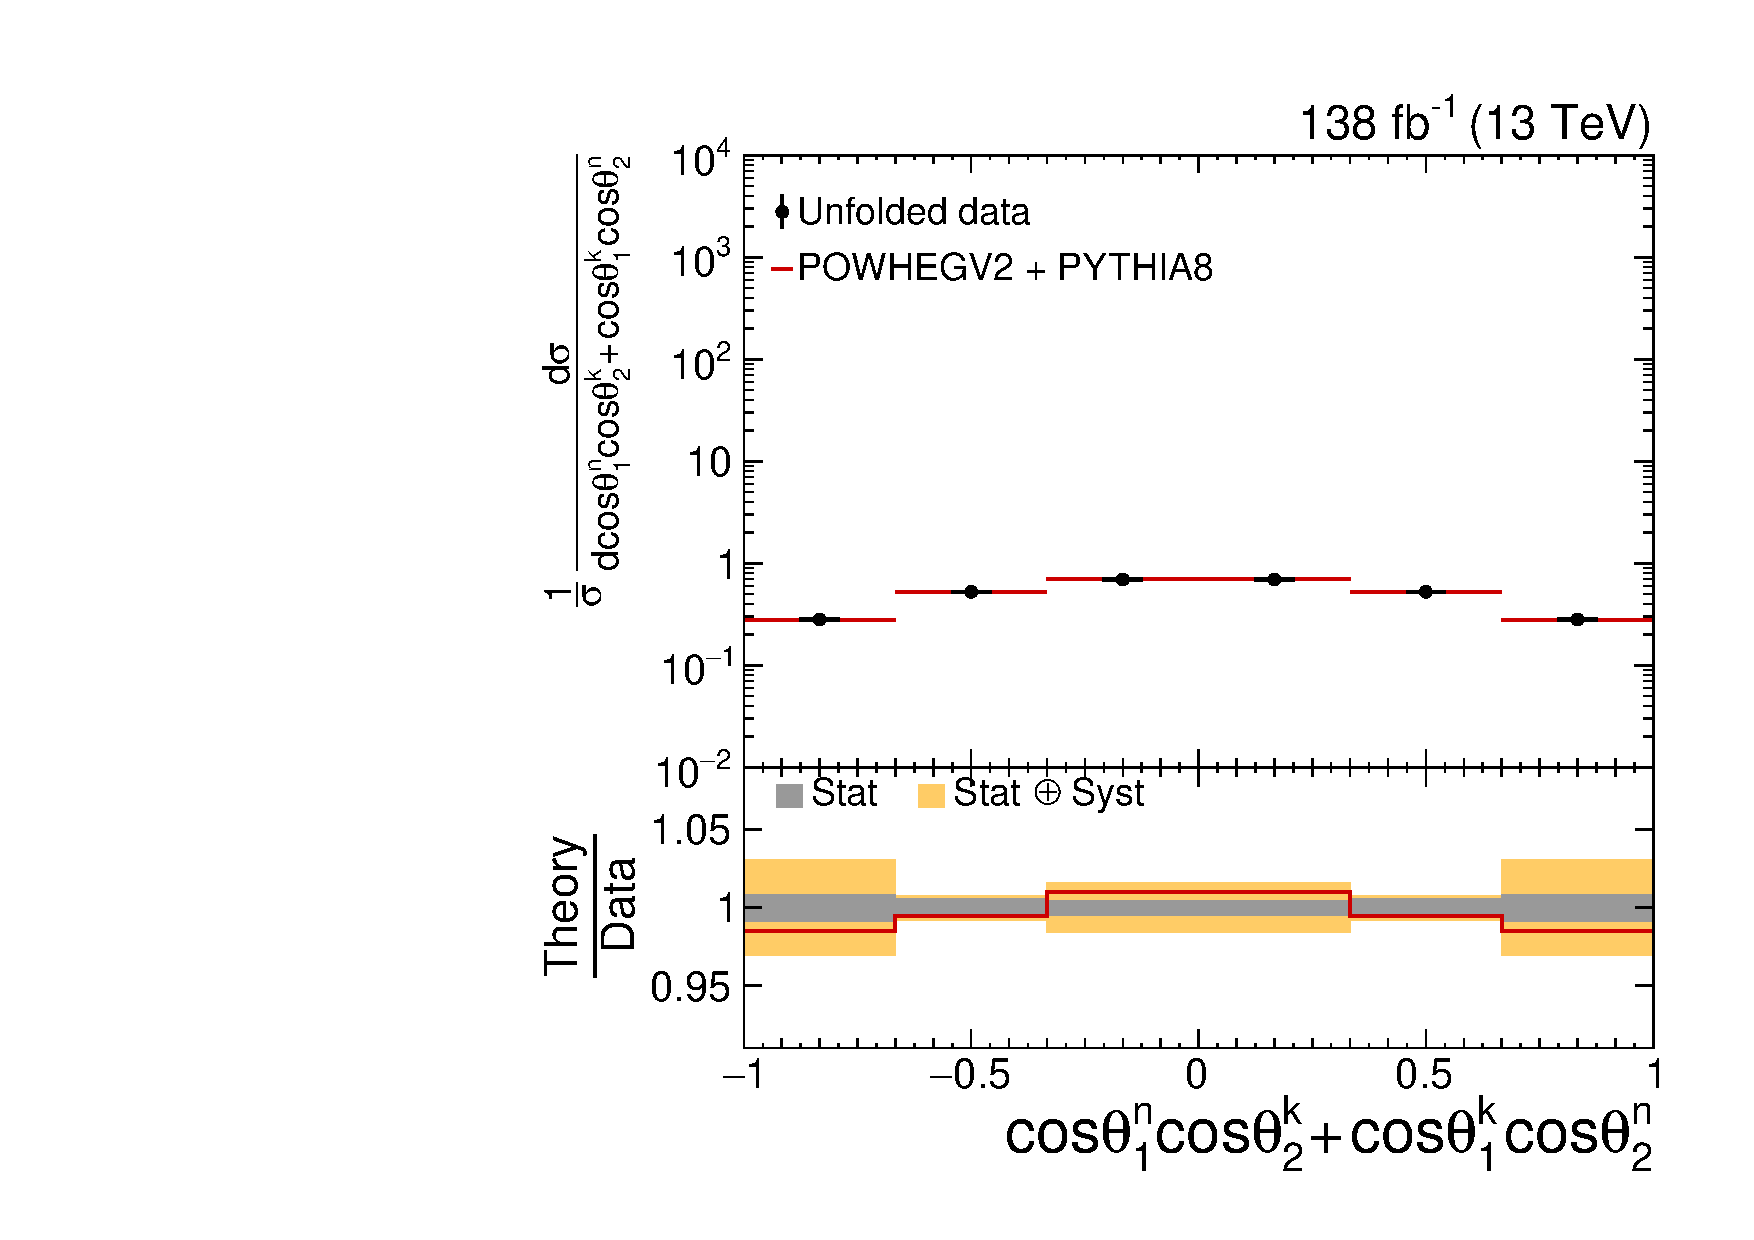
\includegraphics[width=0.40\textwidth]{fig_fullRun2UL/unfolding/combined/UnfoldedResultsNorm_c_Pnk.pdf} \\
\label{fig:c_Pnk}
\caption{Reconstructed detector-level distribution (Top Left), detector response-matrix (Top Right), absolute cross-section unfolded to parton-level (Bottom Left), and normalized cross-section unfolded to parton-level (Bottom Right) for off-diagonal spin correlation sum observable $\cos\theta_{1}^{n}\cos\theta_{2}^{k}+\cos\theta_{1}^{k}\cos\theta_{2}^{n}$, from which spin-density coefficient $C_{nk}+C_{kn}$ (sensitive to spin-density coefficient function $c_{k n}$) is extracted.}
\end{center}
\end{figure}
\clearpage
\begin{figure}[htb]
\begin{center}
 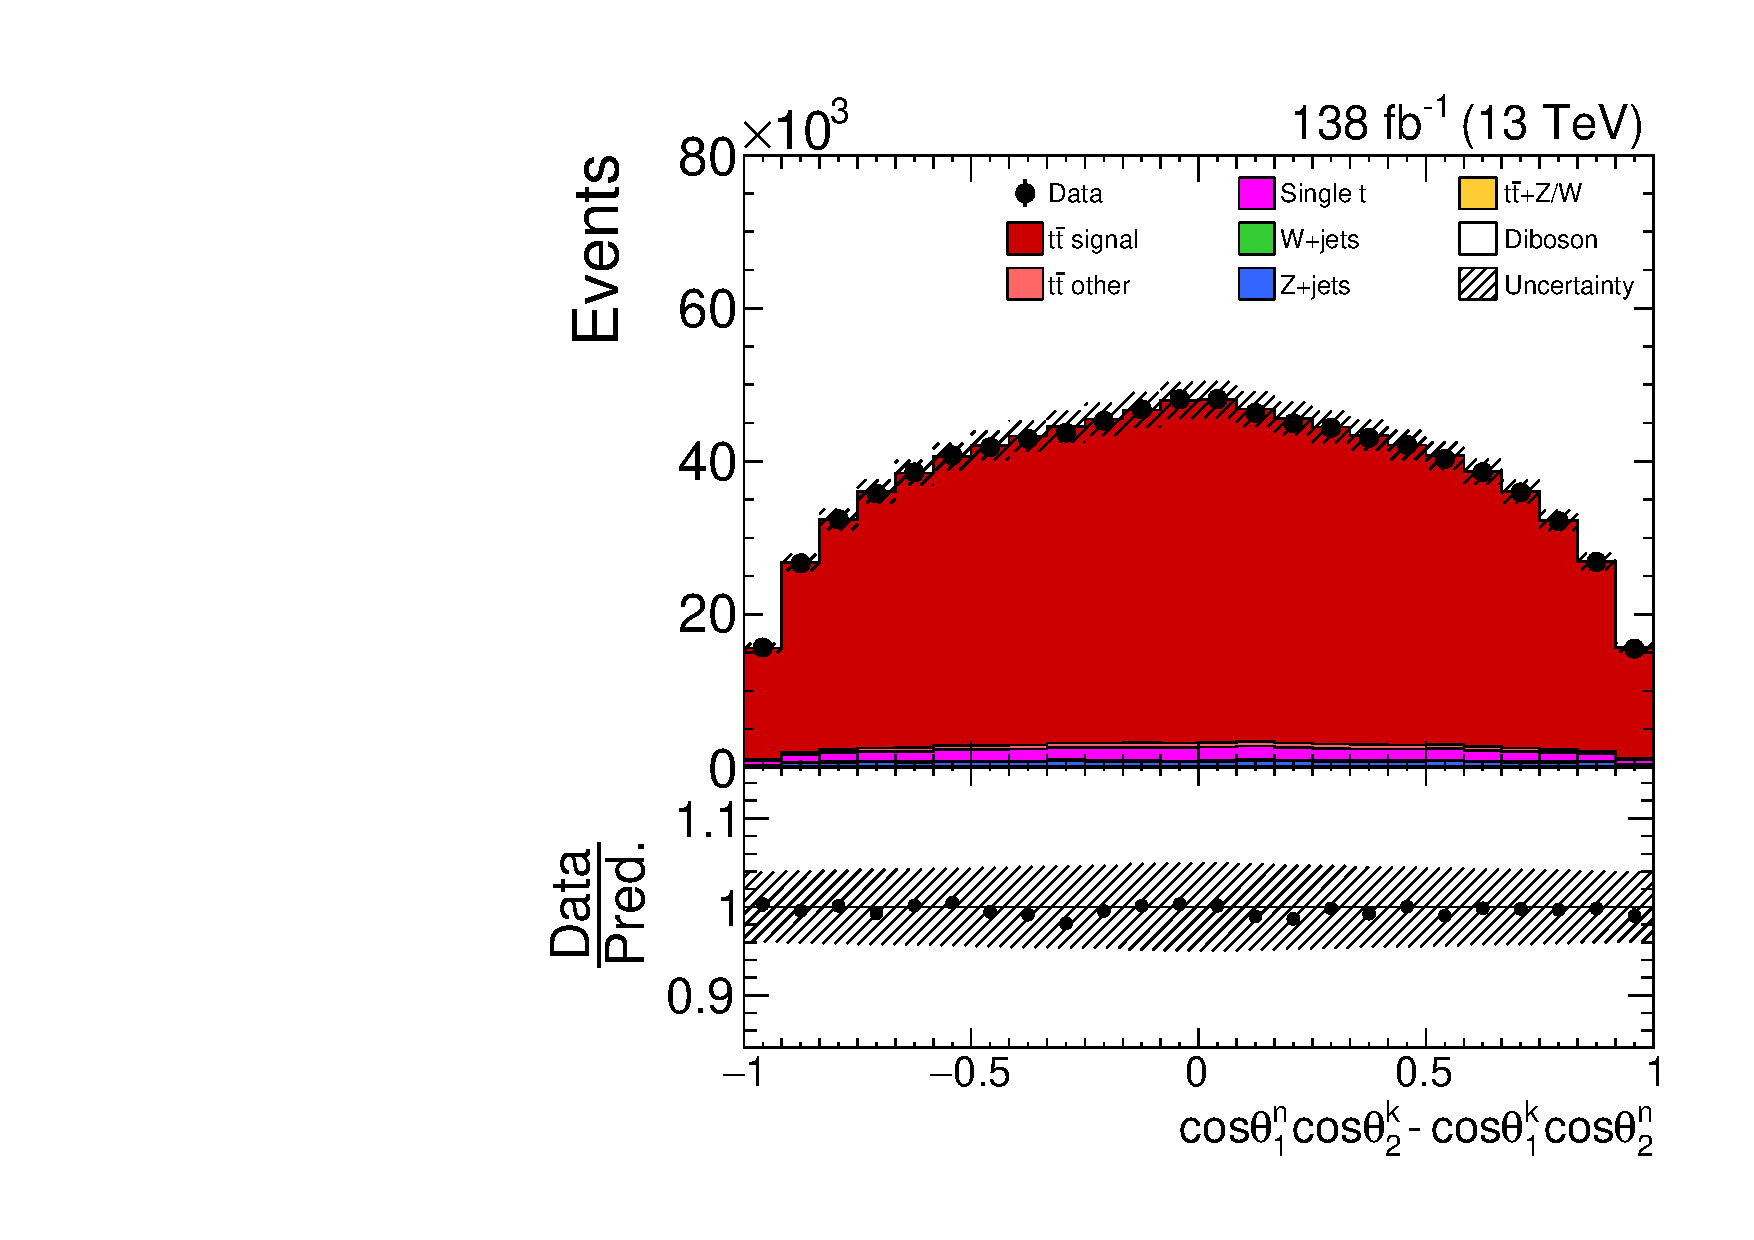
\includegraphics[width=0.40\textwidth]{fig_fullRun2UL/controlplots/combined/Hyp_LLBarCMnk.pdf}
 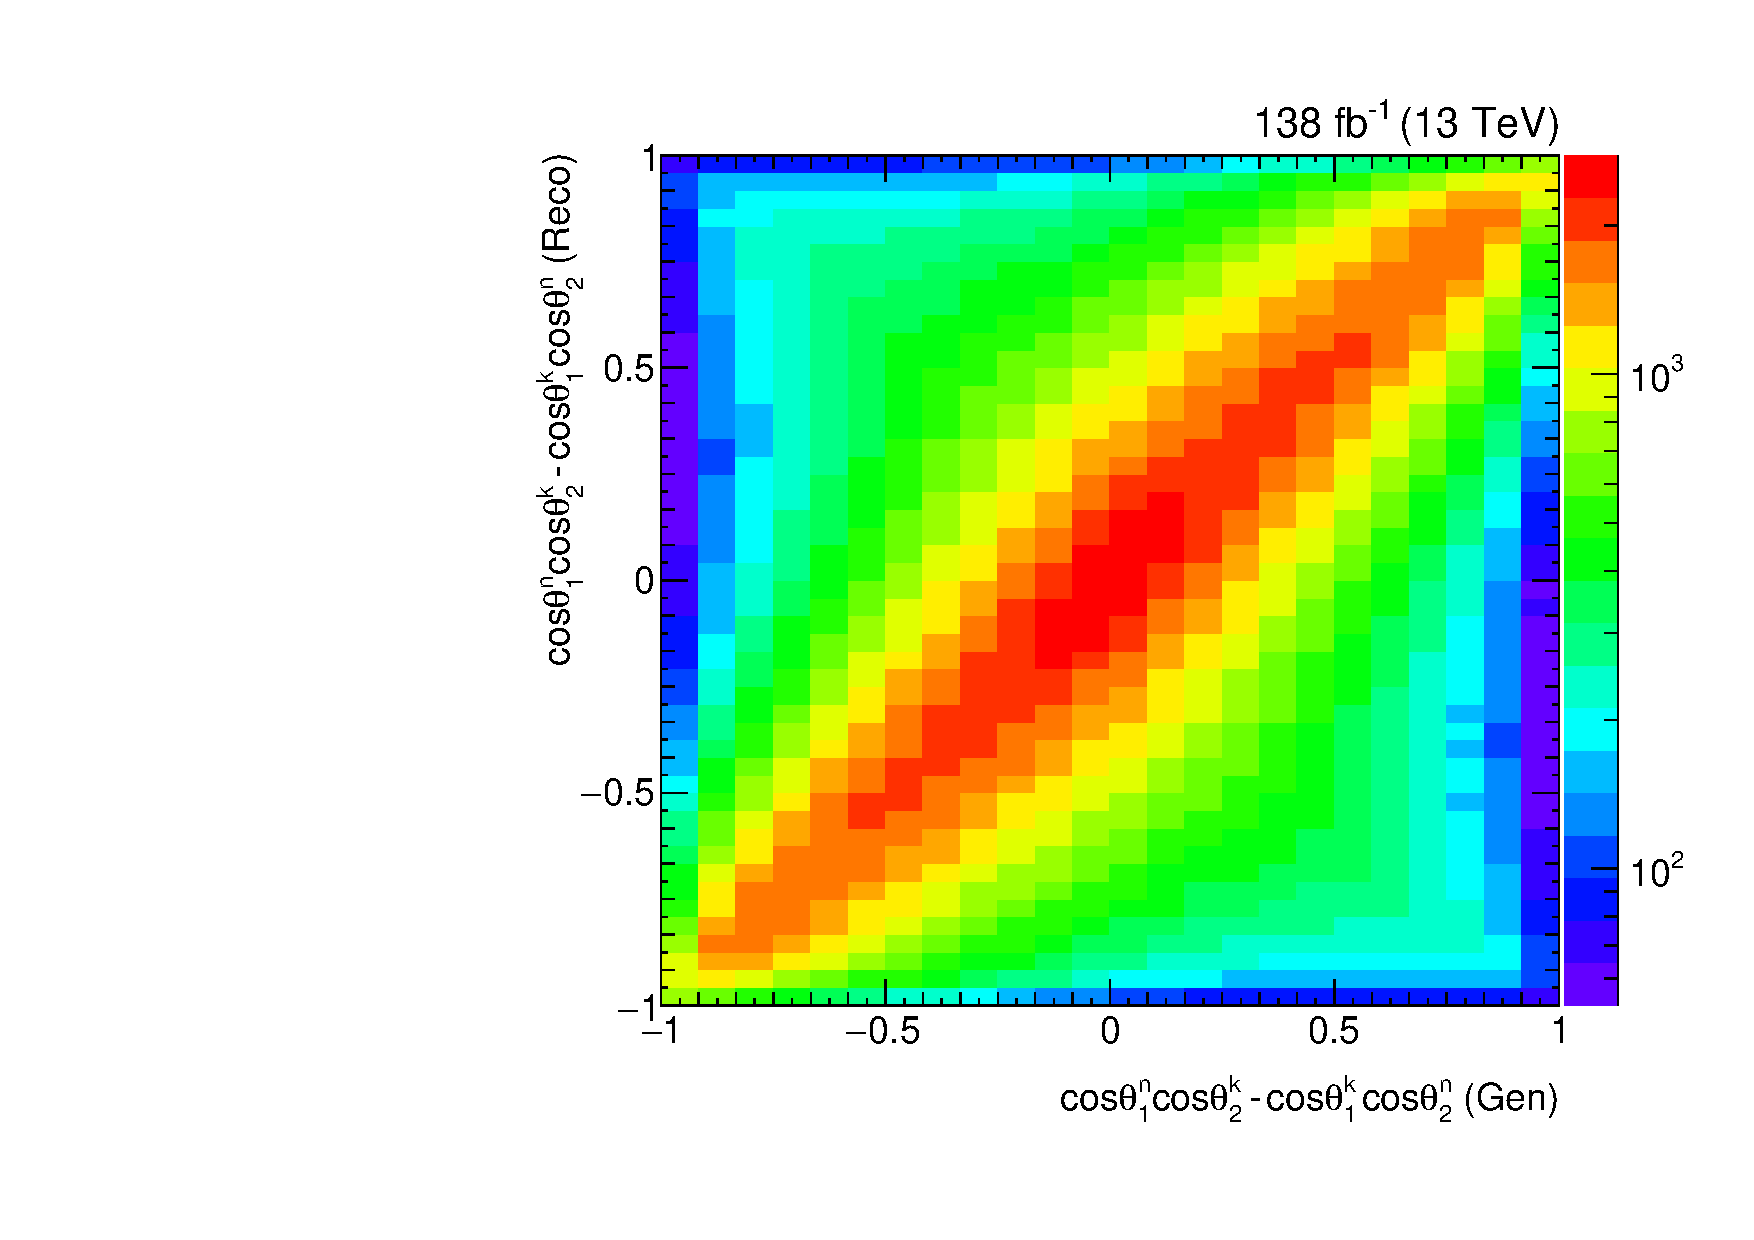
\includegraphics[width=0.40\textwidth]{fig_fullRun2UL/unfolding/combined/ResponseMatrix_c_Mnk.pdf} \\
 \includegraphics[width=0.40\textwidth]{fig_fullRun2UL/unfolding/combined/UnfoldedResults_c_Mnk.pdf}
 \includegraphics[width=0.40\textwidth]{fig_fullRun2UL/unfolding/combined/UnfoldedResultsNorm_c_Mnk.pdf} \\
\label{fig:c_Mnk}
\caption{Reconstructed detector-level distribution (Top Left), detector response-matrix (Top Right), absolute cross-section unfolded to parton-level (Bottom Left), and normalized cross-section unfolded to parton-level (Bottom Right) for off-diagonal spin correlation difference observable $\cos\theta_{1}^{n}\cos\theta_{2}^{k}-\cos\theta_{1}^{k}\cos\theta_{2}^{n}$, from which spin-density coefficient $C_{nk}-C_{kn}$ (sensitive to spin-density coefficient function $-c_r$) is extracted.}
\end{center}
\end{figure}
\clearpage
\begin{figure}[htb]
\begin{center}
 \includegraphics[width=0.40\textwidth]{fig_fullRun2UL/controlplots/combined/Hyp_LLBarcHel.pdf}
 \includegraphics[width=0.40\textwidth]{fig_fullRun2UL/unfolding/combined/ResponseMatrix_ll_cHel.pdf} \\
 \includegraphics[width=0.40\textwidth]{fig_fullRun2UL/unfolding/combined/UnfoldedResults_ll_cHel.pdf}
 \includegraphics[width=0.40\textwidth]{fig_fullRun2UL/unfolding/combined/UnfoldedResultsNorm_ll_cHel.pdf} \\
\label{fig:ll_cHel}
\caption{Reconstructed detector-level distribution (Top Left), detector response-matrix (Top Right), absolute cross-section unfolded to parton-level (Bottom Left), and normalized cross-section unfolded to parton-level (Bottom Right) for  observable $\cos\varphi$, from which spin-density coefficient $D = -\frac{1}{3}(C_{kk} + C_{rr} + C_{nn})$ (sensitive to spin-density coefficient function $-\frac{1}{3}(c_{kk} + c_{rr} + c_{nn})$) is extracted.}
\end{center}
\end{figure}
\clearpage
\begin{figure}[htb]
\begin{center}
 \includegraphics[width=0.40\textwidth]{fig_fullRun2UL/controlplots/combined/Hyp_AntiLeptonBk_vs_TTBarMass.pdf}
 \includegraphics[width=0.40\textwidth]{fig_fullRun2UL/unfolding/combined/ResponseMatrix_b1k_mttbar.pdf} \\
 \includegraphics[width=0.40\textwidth]{fig_fullRun2UL/unfolding/combined/UnfoldedResults_b1k_mttbar.pdf}
 \includegraphics[width=0.40\textwidth]{fig_fullRun2UL/unfolding/combined/UnfoldedResultsNorm_b1k_mttbar.pdf} \\
\label{fig:b1k_mttbar}
\caption{Differential reconstructed detector-level distributions (Top Left), detector response-matrices (Top Right), absolute cross-sections unfolded to parton-level (Bottom Left), and normalized cross-sections unfolded to parton-level (Bottom Right) for polarization observable $\cos\theta_{1}^{k}$ as a function of $m_{t\bar{t}}$, from which differential spin-density coefficients $B_{1}^{k}$ (sensitive to spin-density coefficient functions $b_k^{+}$) are extracted.  The range of the primary axis is applicable to each of the sub-phase space regions partitioned by the grid lines.}
\end{center}
\end{figure}
\clearpage
\begin{figure}[htb]
\begin{center}
 \includegraphics[width=0.40\textwidth]{fig_fullRun2UL/controlplots/combined/Hyp_LeptonBk_vs_TTBarMass.pdf}
 \includegraphics[width=0.40\textwidth]{fig_fullRun2UL/unfolding/combined/ResponseMatrix_b2k_mttbar.pdf} \\
 \includegraphics[width=0.40\textwidth]{fig_fullRun2UL/unfolding/combined/UnfoldedResults_b2k_mttbar.pdf}
 \includegraphics[width=0.40\textwidth]{fig_fullRun2UL/unfolding/combined/UnfoldedResultsNorm_b2k_mttbar.pdf} \\
\label{fig:b2k_mttbar}
\caption{Differential reconstructed detector-level distributions (Top Left), detector response-matrices (Top Right), absolute cross-sections unfolded to parton-level (Bottom Left), and normalized cross-sections unfolded to parton-level (Bottom Right) for polarization observable $\cos\theta_{2}^{k}$ as a function of $m_{t\bar{t}}$, from which differential spin-density coefficients $B_{2}^{k}$ (sensitive to spin-density coefficient functions $b_k^{-}$) are extracted.  The range of the primary axis is applicable to each of the sub-phase space regions partitioned by the grid lines.}
\end{center}
\end{figure}
\clearpage
\begin{figure}[htb]
\begin{center}
 \includegraphics[width=0.40\textwidth]{fig_fullRun2UL/controlplots/combined/Hyp_AntiLeptonBr_vs_TTBarMass.pdf}
 \includegraphics[width=0.40\textwidth]{fig_fullRun2UL/unfolding/combined/ResponseMatrix_b1r_mttbar.pdf} \\
 \includegraphics[width=0.40\textwidth]{fig_fullRun2UL/unfolding/combined/UnfoldedResults_b1r_mttbar.pdf}
 \includegraphics[width=0.40\textwidth]{fig_fullRun2UL/unfolding/combined/UnfoldedResultsNorm_b1r_mttbar.pdf} \\
\label{fig:b1r_mttbar}
\caption{Differential reconstructed detector-level distributions (Top Left), detector response-matrices (Top Right), absolute cross-sections unfolded to parton-level (Bottom Left), and normalized cross-sections unfolded to parton-level (Bottom Right) for polarization observable $\cos\theta_{1}^{r}$ as a function of $m_{t\bar{t}}$, from which differential spin-density coefficients $B_{1}^{r}$ (sensitive to spin-density coefficient functions $b_r^{+}$) are extracted.  The range of the primary axis is applicable to each of the sub-phase space regions partitioned by the grid lines.}
\end{center}
\end{figure}
\clearpage
\begin{figure}[htb]
\begin{center}
 \includegraphics[width=0.40\textwidth]{fig_fullRun2UL/controlplots/combined/Hyp_LeptonBr_vs_TTBarMass.pdf}
 \includegraphics[width=0.40\textwidth]{fig_fullRun2UL/unfolding/combined/ResponseMatrix_b2r_mttbar.pdf} \\
 \includegraphics[width=0.40\textwidth]{fig_fullRun2UL/unfolding/combined/UnfoldedResults_b2r_mttbar.pdf}
 \includegraphics[width=0.40\textwidth]{fig_fullRun2UL/unfolding/combined/UnfoldedResultsNorm_b2r_mttbar.pdf} \\
\label{fig:b2r_mttbar}
\caption{Differential reconstructed detector-level distributions (Top Left), detector response-matrices (Top Right), absolute cross-sections unfolded to parton-level (Bottom Left), and normalized cross-sections unfolded to parton-level (Bottom Right) for polarization observable $\cos\theta_{2}^{r}$ as a function of $m_{t\bar{t}}$, from which differential spin-density coefficients $B_{2}^{r}$ (sensitive to spin-density coefficient functions $b_r^{-}$) are extracted.  The range of the primary axis is applicable to each of the sub-phase space regions partitioned by the grid lines.}
\end{center}
\end{figure}
\clearpage
\begin{figure}[htb]
\begin{center}
 \includegraphics[width=0.40\textwidth]{fig_fullRun2UL/controlplots/combined/Hyp_LLBarCkk_vs_TTBarMass.pdf}
 \includegraphics[width=0.40\textwidth]{fig_fullRun2UL/unfolding/combined/ResponseMatrix_c_kk_mttbar.pdf} \\
 \includegraphics[width=0.40\textwidth]{fig_fullRun2UL/unfolding/combined/UnfoldedResults_c_kk_mttbar.pdf}
 \includegraphics[width=0.40\textwidth]{fig_fullRun2UL/unfolding/combined/UnfoldedResultsNorm_c_kk_mttbar.pdf} \\
\label{fig:c_kk_mttbar}
\caption{Differential reconstructed detector-level distributions (Top Left), detector response-matrices (Top Right), absolute cross-sections unfolded to parton-level (Bottom Left), and normalized cross-sections unfolded to parton-level (Bottom Right) for diagonal spin correlation observable $\cos\theta_{1}^{k}\cos\theta_{2}^{k}$ as a function of $m_{t\bar{t}}$, from which differential spin-density coefficients $C_{kk}$ (sensitive to spin-density coefficient functions $c_{k k}$) are extracted.  The range of the primary axis is applicable to each of the sub-phase space regions partitioned by the grid lines.}
\end{center}
\end{figure}
\clearpage
\begin{figure}[htb]
\begin{center}
 \includegraphics[width=0.40\textwidth]{fig_fullRun2UL/controlplots/combined/Hyp_LLBarCrr_vs_TTBarMass.pdf}
 \includegraphics[width=0.40\textwidth]{fig_fullRun2UL/unfolding/combined/ResponseMatrix_c_rr_mttbar.pdf} \\
 \includegraphics[width=0.40\textwidth]{fig_fullRun2UL/unfolding/combined/UnfoldedResults_c_rr_mttbar.pdf}
 \includegraphics[width=0.40\textwidth]{fig_fullRun2UL/unfolding/combined/UnfoldedResultsNorm_c_rr_mttbar.pdf} \\
\label{fig:c_rr_mttbar}
\caption{Differential reconstructed detector-level distributions (Top Left), detector response-matrices (Top Right), absolute cross-sections unfolded to parton-level (Bottom Left), and normalized cross-sections unfolded to parton-level (Bottom Right) for diagonal spin correlation observable $\cos\theta_{1}^{r}\cos\theta_{2}^{r}$ as a function of $m_{t\bar{t}}$, from which differential spin-density coefficients $C_{rr}$ (sensitive to spin-density coefficient functions $c_{r r}$) are extracted.  The range of the primary axis is applicable to each of the sub-phase space regions partitioned by the grid lines.}
\end{center}
\end{figure}
\clearpage
\begin{figure}[htb]
\begin{center}
 \includegraphics[width=0.40\textwidth]{fig_fullRun2UL/controlplots/combined/Hyp_LLBarCnn_vs_TTBarMass.pdf}
 \includegraphics[width=0.40\textwidth]{fig_fullRun2UL/unfolding/combined/ResponseMatrix_c_nn_mttbar.pdf} \\
 \includegraphics[width=0.40\textwidth]{fig_fullRun2UL/unfolding/combined/UnfoldedResults_c_nn_mttbar.pdf}
 \includegraphics[width=0.40\textwidth]{fig_fullRun2UL/unfolding/combined/UnfoldedResultsNorm_c_nn_mttbar.pdf} \\
\label{fig:c_nn_mttbar}
\caption{Differential reconstructed detector-level distributions (Top Left), detector response-matrices (Top Right), absolute cross-sections unfolded to parton-level (Bottom Left), and normalized cross-sections unfolded to parton-level (Bottom Right) for diagonal spin correlation observable $\cos\theta_{1}^{n}\cos\theta_{2}^{n}$ as a function of $m_{t\bar{t}}$, from which differential spin-density coefficients $C_{nn}$ (sensitive to spin-density coefficient functions $c_{n n}$) are extracted.  The range of the primary axis is applicable to each of the sub-phase space regions partitioned by the grid lines.}
\end{center}
\end{figure}
\clearpage
\begin{figure}[htb]
\begin{center}
 \includegraphics[width=0.40\textwidth]{fig_fullRun2UL/controlplots/combined/Hyp_LLBarCPrk_vs_TTBarMass.pdf}
 \includegraphics[width=0.40\textwidth]{fig_fullRun2UL/unfolding/combined/ResponseMatrix_c_Prk_mttbar.pdf} \\
 \includegraphics[width=0.40\textwidth]{fig_fullRun2UL/unfolding/combined/UnfoldedResults_c_Prk_mttbar.pdf}
 \includegraphics[width=0.40\textwidth]{fig_fullRun2UL/unfolding/combined/UnfoldedResultsNorm_c_Prk_mttbar.pdf} \\
\label{fig:c_Prk_mttbar}
\caption{Differential reconstructed detector-level distributions (Top Left), detector response-matrices (Top Right), absolute cross-sections unfolded to parton-level (Bottom Left), and normalized cross-sections unfolded to parton-level (Bottom Right) for off-diagonal spin correlation sum observable $\cos\theta_{1}^{r}\cos\theta_{2}^{k}+\cos\theta_{1}^{k}\cos\theta_{2}^{r}$ as a function of $m_{t\bar{t}}$, from which differential spin-density coefficients $C_{rk}+C_{kr}$ (sensitive to spin-density coefficient functions $c_{r k}$) are extracted.  The range of the primary axis is applicable to each of the sub-phase space regions partitioned by the grid lines.}
\end{center}
\end{figure}
\clearpage
\begin{figure}[htb]
\begin{center}
 \includegraphics[width=0.40\textwidth]{fig_fullRun2UL/controlplots/combined/Hyp_LLBarCMrk_vs_TTBarMass.pdf}
 \includegraphics[width=0.40\textwidth]{fig_fullRun2UL/unfolding/combined/ResponseMatrix_c_Mrk_mttbar.pdf} \\
 \includegraphics[width=0.40\textwidth]{fig_fullRun2UL/unfolding/combined/UnfoldedResults_c_Mrk_mttbar.pdf}
 \includegraphics[width=0.40\textwidth]{fig_fullRun2UL/unfolding/combined/UnfoldedResultsNorm_c_Mrk_mttbar.pdf} \\
\label{fig:c_Mrk_mttbar}
\caption{Differential reconstructed detector-level distributions (Top Left), detector response-matrices (Top Right), absolute cross-sections unfolded to parton-level (Bottom Left), and normalized cross-sections unfolded to parton-level (Bottom Right) for off-diagonal spin correlation difference observable $\cos\theta_{1}^{r}\cos\theta_{2}^{k}-\cos\theta_{1}^{k}\cos\theta_{2}^{r}$ as a function of $m_{t\bar{t}}$, from which differential spin-density coefficients $C_{rk}-C_{kr}$ (sensitive to spin-density coefficient functions $c_n$) are extracted.  The range of the primary axis is applicable to each of the sub-phase space regions partitioned by the grid lines.}
\end{center}
\end{figure}
\clearpage
\begin{figure}[htb]
\begin{center}
 \includegraphics[width=0.40\textwidth]{fig_fullRun2UL/controlplots/combined/Hyp_LLBarCPnr_vs_TTBarMass.pdf}
 \includegraphics[width=0.40\textwidth]{fig_fullRun2UL/unfolding/combined/ResponseMatrix_c_Pnr_mttbar.pdf} \\
 \includegraphics[width=0.40\textwidth]{fig_fullRun2UL/unfolding/combined/UnfoldedResults_c_Pnr_mttbar.pdf}
 \includegraphics[width=0.40\textwidth]{fig_fullRun2UL/unfolding/combined/UnfoldedResultsNorm_c_Pnr_mttbar.pdf} \\
\label{fig:c_Pnr_mttbar}
\caption{Differential reconstructed detector-level distributions (Top Left), detector response-matrices (Top Right), absolute cross-sections unfolded to parton-level (Bottom Left), and normalized cross-sections unfolded to parton-level (Bottom Right) for off-diagonal spin correlation sum observable $\cos\theta_{1}^{n}\cos\theta_{2}^{r}+\cos\theta_{1}^{r}\cos\theta_{2}^{n}$ as a function of $m_{t\bar{t}}$, from which differential spin-density coefficients $C_{nr}+C_{rn}$ (sensitive to spin-density coefficient functions $c_{n r}$) are extracted.  The range of the primary axis is applicable to each of the sub-phase space regions partitioned by the grid lines.}
\end{center}
\end{figure}
\clearpage
\begin{figure}[htb]
\begin{center}
 \includegraphics[width=0.40\textwidth]{fig_fullRun2UL/controlplots/combined/Hyp_LLBarCMnr_vs_TTBarMass.pdf}
 \includegraphics[width=0.40\textwidth]{fig_fullRun2UL/unfolding/combined/ResponseMatrix_c_Mnr_mttbar.pdf} \\
 \includegraphics[width=0.40\textwidth]{fig_fullRun2UL/unfolding/combined/UnfoldedResults_c_Mnr_mttbar.pdf}
 \includegraphics[width=0.40\textwidth]{fig_fullRun2UL/unfolding/combined/UnfoldedResultsNorm_c_Mnr_mttbar.pdf} \\
\label{fig:c_Mnr_mttbar}
\caption{Differential reconstructed detector-level distributions (Top Left), detector response-matrices (Top Right), absolute cross-sections unfolded to parton-level (Bottom Left), and normalized cross-sections unfolded to parton-level (Bottom Right) for off-diagonal spin correlation difference observable $\cos\theta_{1}^{n}\cos\theta_{2}^{r}-\cos\theta_{1}^{r}\cos\theta_{2}^{n}$ as a function of $m_{t\bar{t}}$, from which differential spin-density coefficients $C_{nr}-C_{rn}$ (sensitive to spin-density coefficient functions $c_k$) are extracted.  The range of the primary axis is applicable to each of the sub-phase space regions partitioned by the grid lines.}
\end{center}
\end{figure}
\clearpage
\begin{figure}[htb]
\begin{center}
 \includegraphics[width=0.40\textwidth]{fig_fullRun2UL/controlplots/combined/Hyp_LLBarCPnk_vs_TTBarMass.pdf}
 \includegraphics[width=0.40\textwidth]{fig_fullRun2UL/unfolding/combined/ResponseMatrix_c_Pnk_mttbar.pdf} \\
 \includegraphics[width=0.40\textwidth]{fig_fullRun2UL/unfolding/combined/UnfoldedResults_c_Pnk_mttbar.pdf}
 \includegraphics[width=0.40\textwidth]{fig_fullRun2UL/unfolding/combined/UnfoldedResultsNorm_c_Pnk_mttbar.pdf} \\
\label{fig:c_Pnk_mttbar}
\caption{Differential reconstructed detector-level distributions (Top Left), detector response-matrices (Top Right), absolute cross-sections unfolded to parton-level (Bottom Left), and normalized cross-sections unfolded to parton-level (Bottom Right) for off-diagonal spin correlation sum observable $\cos\theta_{1}^{n}\cos\theta_{2}^{k}+\cos\theta_{1}^{k}\cos\theta_{2}^{n}$ as a function of $m_{t\bar{t}}$, from which differential spin-density coefficients $C_{nk}+C_{kn}$ (sensitive to spin-density coefficient functions $c_{k n}$) are extracted.  The range of the primary axis is applicable to each of the sub-phase space regions partitioned by the grid lines.}
\end{center}
\end{figure}
\clearpage
\begin{figure}[htb]
\begin{center}
 \includegraphics[width=0.40\textwidth]{fig_fullRun2UL/controlplots/combined/Hyp_LLBarCMnk_vs_TTBarMass.pdf}
 \includegraphics[width=0.40\textwidth]{fig_fullRun2UL/unfolding/combined/ResponseMatrix_c_Mnk_mttbar.pdf} \\
 \includegraphics[width=0.40\textwidth]{fig_fullRun2UL/unfolding/combined/UnfoldedResults_c_Mnk_mttbar.pdf}
 \includegraphics[width=0.40\textwidth]{fig_fullRun2UL/unfolding/combined/UnfoldedResultsNorm_c_Mnk_mttbar.pdf} \\
\label{fig:c_Mnk_mttbar}
\caption{Differential reconstructed detector-level distributions (Top Left), detector response-matrices (Top Right), absolute cross-sections unfolded to parton-level (Bottom Left), and normalized cross-sections unfolded to parton-level (Bottom Right) for off-diagonal spin correlation difference observable $\cos\theta_{1}^{n}\cos\theta_{2}^{k}-\cos\theta_{1}^{k}\cos\theta_{2}^{n}$ as a function of $m_{t\bar{t}}$, from which differential spin-density coefficients $C_{nk}-C_{kn}$ (sensitive to spin-density coefficient functions $-c_r$) are extracted.  The range of the primary axis is applicable to each of the sub-phase space regions partitioned by the grid lines.}
\end{center}
\end{figure}
\clearpage
\begin{figure}[htb]
\begin{center}
 \includegraphics[width=0.40\textwidth]{fig_fullRun2UL/controlplots/combined/Hyp_LLBarcHel_vs_TTBarMass.pdf}
 \includegraphics[width=0.40\textwidth]{fig_fullRun2UL/unfolding/combined/ResponseMatrix_ll_cHel_mttbar.pdf} \\
 \includegraphics[width=0.40\textwidth]{fig_fullRun2UL/unfolding/combined/UnfoldedResults_ll_cHel_mttbar.pdf}
 \includegraphics[width=0.40\textwidth]{fig_fullRun2UL/unfolding/combined/UnfoldedResultsNorm_ll_cHel_mttbar.pdf} \\
\label{fig:ll_cHel_mttbar}
\caption{Differential reconstructed detector-level distributions (Top Left), detector response-matrices (Top Right), absolute cross-sections unfolded to parton-level (Bottom Left), and normalized cross-sections unfolded to parton-level (Bottom Right) for  observable $\cos\varphi$ as a function of $m_{t\bar{t}}$, from which differential spin-density coefficients $D = -\frac{1}{3}(C_{kk} + C_{rr} + C_{nn})$ (sensitive to spin-density coefficient functions $-\frac{1}{3}(c_{kk} + c_{rr} + c_{nn})$) are extracted.  The range of the primary axis is applicable to each of the sub-phase space regions partitioned by the grid lines.}
\end{center}
\end{figure}
\clearpage


\section{Extraction of Coefficients from Differential Cross-Sections}
The coefficients $C$ that parameterize the single-differential cross-sections: 
\begin{linenomath*}
\begin{align}
g(x;C) = (1 \pm Cx)g(x;0)
\end{align}
\end{linenomath*}
are extracted from asymmetries statistics $A_i$ between bins $i$ and $b+1-i$, defined as:
\begin{linenomath*}
\begin{align}
A_i = \frac{N_{b+1-i} - N_i}{N_{b+1-i} + N_i} \quad \text{for} \quad i = 1,2,..,b/2
\end{align}
\end{linenomath*}
where for these measurements $b=6$ is the number of bins for all single-differential cross-sections.
Using the known analytic form of the distribution, as well as the property that the coefficient induces an asymmetry between bins $i$ and $b+1-i$, $A_i$ can be written as:
\begin{linenomath*}
\begin{align}
A_i &= \frac{\int_{bin} (1 \pm C_i x)g(x;0) \; dx  - \int_{bin} (1 \mp C_i x)g(x;0) \; dx}{\int_{bin} (1 \pm C_i x)g(x;0) \; dx  + \int_{bin} (1 \mp C_i x)g(x;0) \; dx} \\
\text{which implies} \quad C_i &= \pm A_i  \frac{\int_{bin} g(x;0) \; dx}{\int_{bin} x g(x;0) \; dx}.
\end{align}
\end{linenomath*}
where $C_i$ is the coefficient extracted from the asymmetry between bins $i$ and $b+1-i$, and the integrals over the bin region $\int_{bin} g(x;0) \; dx$ and $\int_{bin} x g(x;0) \; dx$ are evaluated using Mathematica.
The $C_i$ measurements, with covariance matrix $V^C$, can be combined for an optimal weighted measurement of $C$:
\begin{linenomath*}
\begin{align*}
C &= \frac{\sum_i C_i a_i}{\sum_i a_i} \quad \quad \sigma^2_C = \frac{\vec{a}^T V^C \vec{a}}{\left( \sum_i a_i \right)^2}
\end{align*}
\end{linenomath*}
with weights $a_i$ determined by minimizing the variance of the combined measurement $\sigma^2_C$:
\begin{linenomath*}
\begin{align*}
  a_1 &= \frac{b_1}{b_1+b_2+b_3} \quad \quad & b_1 &= V^C_{2,2}V^C_{3,3} - V^C_{2,3}V^C_{2,3} - V^C_{1,2}(V^C_{3,3}-V^C_{2,3}) - V^C_{1,3}(V^C_{2,2}-V^C_{2,3}) \\
  a_2 &= \frac{b_2}{b_1+b_2+b_3} \quad \text{where} \quad & b_2 &= V^C_{1,1}V^C_{3,3} - V^C_{1,3}V^C_{1,3} - V^C_{1,2}(V^C_{3,3}-V^C_{1,3}) - V^C_{2,3}(V^C_{1,1}-V^C_{1,3}) \\
  a_3 &= \frac{b_3}{b_1+b_2+b_3} \quad \quad & b_3 &= V^C_{1,1}V^C_{2,2} - V^C_{1,2}V^C_{1,2} - V^C_{1,3}(V^C_{2,2}-V^C_{1,2}) - V^C_{2,3}(V^C_{1,1}-V^C_{1,2}) \\
\end{align*}
\end{linenomath*}
For small coefficients, these statistics can be shown to satisfy the Cramér-Rao bound and provide the minimum variances for unbiased estimators of the coefficients.
For double differential measurements as a function of $m_{\ttbar}$, the coefficient extraction procedure is performed in an identical way in each of the sub-phase space regions partitioned by the $m_{\ttbar}$ bin boundaries.


\begin{table}[htb]
    \centering
\begin{tabular}{l | c c}
\hline
\textbf{Coefficient} & \textbf{Measured} & \textbf{\Powheg} \\
$B_{1}^{k}$ & $0.000 \pm 0.002$ & $-0.000^{+0.000}_{-0.000}$ \\
$B_{2}^{k}$ & $-0.000 \pm 0.002$ & $-0.000^{+0.000}_{-0.000}$ \\
$B_{1}^{r}$ & $0.000 \pm 0.003$ & $-0.000^{+0.000}_{-0.000}$ \\
$B_{2}^{r}$ & $0.000 \pm 0.003$ & $-0.000^{+0.000}_{-0.000}$ \\
$B_{1}^{n}$ & $-0.000 \pm 0.003$ & $-0.000^{+0.000}_{-0.000}$ \\
$B_{2}^{n}$ & $-0.000 \pm 0.003$ & $-0.000^{+0.000}_{-0.000}$ \\
$C_{kk}$ & $0.000 \pm 0.005$ & $-0.000^{+0.330}_{-0.000}$  \\
$C_{rr}$ & $0.000 \pm 0.006$ & $-0.000^{+0.330}_{-0.000}$ \\
$C_{nn}$ & $0.000 \pm 0.003$ & $-0.000^{+0.330}_{-0.000}$ \\
$C_{rk}+C_{kr}$ & $0.000 \pm 0.010$ & $-0.000^{+0.061}_{-0.000}$ \\
$C_{rk}-C_{kr}$ & $-0.000 \pm 0.010$ & $-0.000^{+0.060}_{-0.000}$ \\
$C_{nr}+C_{rn}$ & $-0.000 \pm 0.008$ & $-0.000^{+0.060}_{-0.000}$ \\
$C_{nr}-C_{rn}$ & $0.000 \pm 0.008$ & $-0.000^{+0.060}_{-0.000}$ \\
$C_{nk}+C_{kn}$ & $0.000 \pm 0.009$ & $-0.000^{+0.060}_{-0.000}$ \\
$C_{nk}-C_{kn}$ & $-0.000 \pm 0.007$ & $-0.000^{+0.060}_{-0.000}$ \\
$D$ & $-0.000 \pm 0.002$ & $0.000^{+0.000}_{-0.000}$ \\
\hline
\end{tabular}
    \caption{Caption}
    \label{tab:Extracted_Coefficients_1D}
\end{table}

\begin{table}[htb]
    \centering
\begin{tabular}{l | c c}
\hline
\textbf{Coefficient} & \textbf{Measured} & \textbf{\Powheg} \\
$B^{k}_{1, 250 < m_{t\bar{t}} < 450}$ & $0.000 \pm 0.012$ & $-0.000^{+0.000}_{-0.000}$  \\
$B^{k}_{1, 450 < m_{t\bar{t}} < 600}$ & $-0.000 \pm 0.010$ & $-0.000^{+0.000}_{-0.000}$  \\
$B^{k}_{1, 600 < m_{t\bar{t}} < 800}$ & $-0.000 \pm 0.022$ & $-0.000^{+0.000}_{-0.000}$  \\
$B^{k}_{1, 800 < m_{t\bar{t}} < 2000}$ & $-0.000 \pm 0.021$ & $-0.000^{+0.000}_{-0.000}$  \\
$B^{k}_{2, 250 < m_{t\bar{t}} < 450}$ & $-0.000 \pm 0.012$ & $-0.000^{+0.000}_{-0.000}$  \\
$B^{k}_{2, 450 < m_{t\bar{t}} < 600}$ & $-0.000 \pm 0.010$ & $-0.000^{+0.000}_{-0.000}$  \\
$B^{k}_{2, 600 < m_{t\bar{t}} < 800}$ & $0.000 \pm 0.021$ & $0.000^{+0.000}_{-0.000}$  \\
$B^{k}_{2, 800 < m_{t\bar{t}} < 2000}$ & $0.000 \pm 0.023$ & $-0.000^{+0.000}_{-0.000}$  \\
$B^{r}_{1, 250 < m_{t\bar{t}} < 450}$ & $0.000 \pm 0.030$ & $-0.000^{+0.000}_{-0.000}$  \\
$B^{r}_{1, 450 < m_{t\bar{t}} < 600}$ & $-0.000 \pm 0.014$ & $-0.000^{+0.000}_{-0.000}$  \\
$B^{r}_{1, 600 < m_{t\bar{t}} < 800}$ & $0.000 \pm 0.029$ & $-0.000^{+0.000}_{-0.000}$  \\
$B^{r}_{1, 800 < m_{t\bar{t}} < 2000}$ & $-0.000 \pm 0.027$ & $-0.000^{+0.000}_{-0.000}$  \\
$B^{r}_{2, 250 < m_{t\bar{t}} < 450}$ & $0.000 \pm 0.029$ & $-0.000^{+0.000}_{-0.000}$  \\
$B^{r}_{2, 450 < m_{t\bar{t}} < 600}$ & $-0.000 \pm 0.014$ & $-0.000^{+0.000}_{-0.000}$  \\
$B^{r}_{2, 600 < m_{t\bar{t}} < 800}$ & $-0.000 \pm 0.029$ & $0.000^{+0.000}_{-0.000}$  \\
$B^{r}_{2, 800 < m_{t\bar{t}} < 2000}$ & $0.000 \pm 0.026$ & $-0.000^{+0.000}_{-0.000}$  \\
$B^{n}_{1, 250 < m_{t\bar{t}} < 450}$ & $-0.000 \pm 0.058$ & $-0.000^{+0.000}_{-0.000}$  \\
$B^{n}_{1, 450 < m_{t\bar{t}} < 600}$ & $-0.000 \pm 0.012$ & $-0.000^{+0.000}_{-0.000}$  \\
$B^{n}_{1, 600 < m_{t\bar{t}} < 800}$ & $0.000 \pm 0.026$ & $-0.000^{+0.000}_{-0.000}$  \\
$B^{n}_{1, 800 < m_{t\bar{t}} < 2000}$ & $0.000 \pm 0.022$ & $0.000^{+0.000}_{-0.000}$  \\
$B^{n}_{2, 250 < m_{t\bar{t}} < 450}$ & $-0.000 \pm 0.065$ & $-0.000^{+0.000}_{-0.000}$  \\
$B^{n}_{2, 450 < m_{t\bar{t}} < 600}$ & $-0.000 \pm 0.012$ & $-0.000^{+0.000}_{-0.000}$  \\
$B^{n}_{2, 600 < m_{t\bar{t}} < 800}$ & $0.000 \pm 0.027$ & $-0.000^{+0.000}_{-0.000}$  \\
$B^{n}_{2, 800 < m_{t\bar{t}} < 2000}$ & $0.000 \pm 0.022$ & $-0.000^{+-nan}_{-0.000}$  \\
\hline
\end{tabular}
    \caption{Caption}
    \label{tab:Extracted_Coefficients_2D_Polarizations}
\end{table}

\begin{table}[htb]
    \centering
\begin{tabular}{l | c c}
\hline
\textbf{Coefficient} & \textbf{Measured} & \textbf{\Powheg} \\
$C_{kk, 250 < m_{t\bar{t}} < 450}$ & $0.000 \pm 0.015$ & $-0.000^{+0.000}_{-0.000}$  \\
$C_{kk, 450 < m_{t\bar{t}} < 600}$ & $-0.000 \pm 0.019$ & $-0.000^{+0.000}_{-0.000}$  \\
$C_{kk, 600 < m_{t\bar{t}} < 800}$ & $-0.000 \pm 0.036$ & $-0.000^{+0.000}_{-0.000}$  \\
$C_{kk, 800 < m_{t\bar{t}} < 2000}$ & $-0.000 \pm 0.065$ & $-0.000^{+0.001}_{-0.001}$  \\
$C_{rr, 250 < m_{t\bar{t}} < 450}$ & $0.000 \pm 0.024$ & $0.000^{+0.000}_{-0.000}$  \\
$C_{rr, 450 < m_{t\bar{t}} < 600}$ & $0.000 \pm 0.024$ & $0.000^{+0.000}_{-0.000}$  \\
$C_{rr, 600 < m_{t\bar{t}} < 800}$ & $-0.000 \pm 0.052$ & $-0.000^{+0.000}_{-0.000}$  \\
$C_{rr, 800 < m_{t\bar{t}} < 2000}$ & $0.000 \pm 0.092$ & $0.000^{+0.001}_{--nan}$  \\
$C_{nn, 250 < m_{t\bar{t}} < 450}$ & $0.000 \pm 0.041$ & $0.000^{+0.000}_{-0.000}$  \\
$C_{nn, 450 < m_{t\bar{t}} < 600}$ & $0.000 \pm 0.033$ & $-0.000^{+0.000}_{-0.000}$  \\
$C_{nn, 600 < m_{t\bar{t}} < 800}$ & $-0.000 \pm 0.064$ & $-0.000^{+0.000}_{-0.000}$  \\
$C_{nn, 800 < m_{t\bar{t}} < 2000}$ & $-0.000 \pm 0.075$ & $-0.000^{+0.001}_{-0.001}$  \\
$(C_{rk}+C_{kr})_{250 < m_{t\bar{t}} < 450}$ & $-0.000 \pm 0.034$ & $-0.000^{+0.000}_{-0.000}$  \\
$(C_{rk}+C_{kr})_{450 < m_{t\bar{t}} < 600}$ & $-0.000 \pm 0.034$ & $-0.000^{+0.000}_{-0.000}$  \\
$(C_{rk}+C_{kr})_{600 < m_{t\bar{t}} < 800}$ & $0.000 \pm 0.072$ & $-0.000^{+0.001}_{-0.001}$  \\
$(C_{rk}+C_{kr})_{800 < m_{t\bar{t}} < 2000}$ & $0.000 \pm 0.094$ & $0.000^{+0.001}_{-0.001}$  \\
$(C_{rk}-C_{kr})_{250 < m_{t\bar{t}} < 450}$ & $0.000 \pm 0.172$ & $-0.000^{+0.000}_{-0.000}$  \\
$(C_{rk}-C_{kr})_{450 < m_{t\bar{t}} < 600}$ & $0.000 \pm 0.034$ & $-0.000^{+0.000}_{-0.000}$  \\
$(C_{rk}-C_{kr})_{600 < m_{t\bar{t}} < 800}$ & $0.000 \pm 0.068$ & $-0.000^{+0.001}_{-0.001}$  \\
$(C_{rk}-C_{kr})_{800 < m_{t\bar{t}} < 2000}$ & $0.000 \pm 0.079$ & $-0.000^{+0.001}_{-0.001}$  \\
$(C_{nr}+C_{rn})_{250 < m_{t\bar{t}} < 450}$ & $0.000 \pm 0.103$ & $-0.000^{+0.000}_{-0.000}$  \\
$(C_{nr}+C_{rn})_{450 < m_{t\bar{t}} < 600}$ & $0.000 \pm 0.033$ & $-0.000^{+0.000}_{-0.000}$  \\
$(C_{nr}+C_{rn})_{600 < m_{t\bar{t}} < 800}$ & $0.000 \pm 0.070$ & $-0.000^{+0.001}_{-0.001}$  \\
$(C_{nr}+C_{rn})_{800 < m_{t\bar{t}} < 2000}$ & $0.000 \pm 0.076$ & $-0.000^{+0.001}_{-0.001}$  \\
$(C_{nr}-C_{rn})_{250 < m_{t\bar{t}} < 450}$ & $-0.000 \pm 0.100$ & $-0.000^{+0.000}_{-0.000}$  \\
$(C_{nr}-C_{rn})_{450 < m_{t\bar{t}} < 600}$ & $-0.000 \pm 0.031$ & $-0.000^{+0.000}_{-0.000}$  \\
$(C_{nr}-C_{rn})_{600 < m_{t\bar{t}} < 800}$ & $0.000 \pm 0.071$ & $-0.000^{+0.001}_{-0.001}$  \\
$(C_{nr}-C_{rn})_{800 < m_{t\bar{t}} < 2000}$ & $0.000 \pm 0.076$ & $-0.000^{+0.001}_{-0.001}$  \\
$(C_{nk}+C_{kn})_{250 < m_{t\bar{t}} < 450}$ & $0.000 \pm 0.275$ & $-0.000^{+0.000}_{-0.000}$  \\
$(C_{nk}+C_{kn})_{450 < m_{t\bar{t}} < 600}$ & $0.000 \pm 0.031$ & $-0.000^{+0.000}_{-0.000}$  \\
$(C_{nk}+C_{kn})_{600 < m_{t\bar{t}} < 800}$ & $0.000 \pm 0.064$ & $-0.000^{+0.001}_{-0.001}$  \\
$(C_{nk}+C_{kn})_{800 < m_{t\bar{t}} < 2000}$ & $-0.000 \pm 0.073$ & $-0.000^{+0.001}_{-0.001}$  \\
$(C_{nk}-C_{kn})_{250 < m_{t\bar{t}} < 450}$ & $0.000 \pm 0.057$ & $-0.000^{+0.000}_{-0.000}$  \\
$(C_{nk}-C_{kn})_{450 < m_{t\bar{t}} < 600}$ & $-0.000 \pm 0.028$ & $-0.000^{+0.000}_{-0.000}$  \\
$(C_{nk}-C_{kn})_{600 < m_{t\bar{t}} < 800}$ & $0.000 \pm 0.056$ & $-0.000^{+0.001}_{-0.001}$  \\
$(C_{nk}-C_{kn})_{800 < m_{t\bar{t}} < 2000}$ & $0.000 \pm 0.071$ & $-0.000^{+0.001}_{-0.001}$  \\
$D_{250 < m_{t\bar{t}} < 450}$ & $-0.000 \pm 0.006$ & $0.000^{+0.000}_{-0.000}$  \\
$D_{450 < m_{t\bar{t}} < 600}$ & $-0.000 \pm 0.010$ & $0.000^{+0.000}_{-0.000}$  \\
$D_{600 < m_{t\bar{t}} < 800}$ & $0.000 \pm 0.023$ & $0.000^{+0.000}_{-0.000}$  \\
$D_{800 < m_{t\bar{t}} < 2000}$ & $0.000 \pm 0.025$ & $0.000^{+0.000}_{-0.000}$  \\
\hline
\end{tabular}
    \caption{Caption}
    \label{tab:Extracted_Coefficients_2D_Spin_Correlations}
\end{table}

\clearpage